\chapter{A new solution}
\label{cha:new_solution}

In the last chapter, we introduced several different approaches to the problem of allocation.
And in this chapter, we introduce a new solution that builds apon some elements of the previous solutions.

Particularly we develop a solution concept that extends Nash bargaining with endogenous disagreement point (from section \ref{sec:solutions_bargaining}) to a coalitional schema accommodating arbitrary numbers of players.
The solution we give extends the work of others to the space of generalized non-cooperative games, which are then suitable for describing various applications in electricity network situations.
Our new solution concept is called the GNK value, and is computed and compared against other solutions of the previous chapter - particularly, the Shapley Value, LMP and VCG.
We particularly focus in the calculation and results in the Optimal Power Flow (OPF) setting.
It is seen that through this comparrison, that the different solution concepts give rather different outcomes; and we discuss these differences in light of our ethical considerations (from Chapter \ref{cha:background}).

\section{Prelude to the GNK value}

In the previous section we introduced several solution concepts, each stemming from different principles and having ethical associations and perspective.

In this section we outlay a new approach that combines some of the features of the solution concepts outlayed in the previous chapter.
The primary motivation for this new solution, is to attempt to rarefy the intuition behind the Nash bargaining solution concepts (per secton \ref{sec:solutions_bargaining}) into a more full-blooded description of total allocation, suitable for arbitrary number of players - rather than just two.
In Nash bargaining solution, the minimax payoff advantage between two parties is considered as a measure of bargaining strength, and so we consider the minimax payoff advantages that could occur in bargaining between all possible coalitions of players.
We then allocate power and utility to players directly in proportion to these bargaining strengths using Shapley Value axioms.
In this way we consider and allocate in proportion to the leverage that all the individuals - and groups of individuals - could hypothetically posses in bargaining for outcomes they desire.

Our approach straightforwardly relates to many of the concepts of the previous section: where we have a fundamentally coalitional scheme (per Coalitional Game Theory), that rewards based upon disagreement points (Bargaining Theory), which is partially informed by how much individual's participation influences the group's well-being (reminiscent of VCG), and attempts to describe normative trading between large numbers of participants (Marginalism).

%As already stated (in the bargaining section \ref{sec:solutions_bargaining}), Nash's bargaining solutions attempt to mathematically describe outcomes that are a result of idealised competition under equilibrium, and hence can serve as a description of normalised trading;
%and our new GNK solution concept is similar.
%The reasons why this is potentially usefull, is that such normalised trading can potentially be a measure of what can (or could) be ethically expected of any market agent.

%much more than they are necessarily prescriptive outcomes of an idealised ethics.
%Though the two (ideal competitive outcomes and ethical outcomes) may be related, or even identical in certain contexts - such as where no particular ethical principles apply or the purpose of the engagement is the competition (such as in sports).
%And it is in this same way that the Marginalism outlined in Section \ref{} is often primarily treated usually begin descriptive than prescriptive.

%However there is a line of ethical thinking that idealises competition as being associated-with or determining appropriate ethics; as we consider in Section \ref{}, and for those inclined to think that way then our solution is all the more relevant.
%In anycase, the process of crafting better (or different) descriptions of competitive outcomes is not to be feared, as it may be usefull for describing situations as they might occur under free competition, or as a starting point for implementation in arenas without or prior-to relevant ethical concerns.

Let us begin.

\section{Introduction to the GNK value}

How should we model ideal competition? In the two player case, existing bargaining solutions (such as Nash's) seem rather difficult to surpass. As they describe a singular and axiomatic outcome that is both cooperatively pareto-optimal and also driven by perfect anti-cooperative strategising.

In the context of nash bargaining with endogenous disagreement point (per section \ref{subsec:nash_bargaining_endogenous}), the disagreement point was interpreted as a unique point defined by a minimax equilibrium in the payoff-advantage of strategies.
However there exists a problem extending this scheme directly to three or more players, as there may not always a unique minimax equilibrium in payoff-advantages for strategies in a game of three-or-more players.
The question then is how to logically and consistently extend Nash's bargaining solution with endogenous disagreement point to an arbitrary number of players?

While it may be possible to simply declare one of thoes possible minimax equilibria in a 3+ person game as the disagreement point, 
instead we consider all the possible divisions of players between two groups and then consider all the two-player minimax payoff advantages between them. And the we integrate this information via Shapley Value axioms to form a unique outcome.

In the following sections we give all the details of this process.% Particularly we note that this process of how to reasonably extend Nash's bargaining solution to multiple players has a history.

The fundamental idea behind our approach was first detailed by John Harsanyi in 1963 \cite{values3}.
So far as we know, Harsanyi's solution concepts have never been applied to electricity networks, as there exists a particular problem in doing so, particularly that Harsanyi's solution concepts apply to non-cooperative games but cannot apply to generalised non-cooperative games.
The details of this problem and our novel remedy are spelled out in following sections.

But briefly, that in many electricity network contexts the mutual interactions of participants are limited.
And these limitations on the space of possible mutual actions is best modelled by a generalized noncooperative game, and unfortunately in the context of such a generalized game there is no unique minimax point between two players.
Our principle and novel development in this chapter is the provision of a remedy, such that Harsanyi's solution can then be applied.

The remedy is to take the expected outcome on a coin-flip on who chooses actions first in the minimax strategies - and as we shall see - this turns out to be a unique value that satisfies all required properties, and thus leads to a coherent outcome.

The resulting outcome we call the \textit{Generalized Neymann and Kohlberg Value} or the \textit{GNK value} for short, 
as Harsanyi's solution was also axiomatically derived by Neynamm and Kohlberg.\cite{value2,KOHLBERG2018139}
This solution concept is shown to apply for all transferrable utility (TU) generalized non-cooperative games.

The GNK value is thus flexible enough to extend to many contexts, but we focus particularly on the case of allocating monetary payments over Optimal Power Flow (OPF) instances.
Let us derive the GNK value before giving details of its application.

\section{Deriving the GNK value}\label{the_value_def2}

We begin by presenting the axiomatic foundations of the GNK value, starting from the same point as Neyman and Kohlberg's exposition \cite{value2}.
We begin by defining the the GNK value to be the integration of \emph{threat} values between possible coalitions; defined via Shapley value axioms.
We then describe the \emph{threat} or \emph{advantage} of a coalition $v(S)$ in the context of a \textit{generalized non-cooperative game} (which is our key point of novelty in the solution concept).

And then we clarify how the GNK value relates to other prominent solution concepts in non-cooperative games.

\subsection{Axiomatic foundations and the \textit{Value}}\label{the_value_def}

%There have been many attempts to answer the question of what cooperative outcome \textit{should} occur in the context of a non-cooperative TU game.
%One well known answer is the \textit{Nash bargaining solution} between two players \cite{nash2}, which Harsanyi extended to arbitrary numbers of players.
%Building on this, Harsanyi's solution \cite{values3} was derived from a simple set of axioms by Neyman and Kohlberg ~\cite{value2}; 
%our axiomatic derivation of a value for games with generalized action spaces mirrors the steps in theirs.

We begin by considering Neyman and Kohlberg's \textit{coalitional game of threats} \cite{KOHLBERG2018139}, 
which is a coalitional game defined by a pair $\langle N,v \rangle$ in which:
\begin{itemize}
\item	$N=\{1,\dots,n\}$ is a finite set of \textit{players} or \textit{agents}, and
\item	$v:2^N\rightarrow \mathbb{R}$ is a \textit{characteristic function} with 
\begin{equation}
v(S)=-v(N\setminus S) \label{myeq2} \quad \forall S\subseteq N.
\end{equation}
\end{itemize}
The intuition for \eqref{myeq2} is that the characteristic function of this game is an measure of the strength of the bargaining position (the ``threat'' or ``advantage'') that a coalition, $S$, has over its complement, $N\setminus S$.
This contrasts against classical cooperative game theory games, where the characteristic function $v(\emptyset)=0$ and equation \ref{myeq2} does not generally hold (see section \ref{sec:cooperative_game_theory_part}).

Neyman and Kohlberg's key result was to prove that if $\mathbb{D}$ is the set of all such games, then there exists a unique mapping $\varphi:\mathbb{D}\rightarrow\mathbb{R}^n$ that satisfies the following four axioms:

\begin{itemize}
\item	\textbf{Efficiency}: $\sum_i\varphi(\langle N,v\rangle)_i = v(N)~~~~~\refstepcounter{equation}(\theequation)\label{myeq}$
\item	\textbf{Symmetry}: If two players $i$ and $j$ are substitutes, such that if $v(S\cup i)=v(S\cup j)~~\forall S\subseteq N\setminus\{i,j\}$, then $\varphi(\langle N,v\rangle)_i = \varphi(\langle N,v\rangle)_j$
\item	\textbf{Null Player}: If a player $i$ is a null player (i.e.\ $v(S\cup i)=v(S)~~\forall S\subseteq N$) then $\varphi(\langle N,v\rangle)_i=0$
\item	\textbf{Additivity}: for any $v_1$ and $v_2$, $\varphi(\langle N,v_1+v_2\rangle)=\varphi(\langle N,v_1 \rangle) + \varphi(\langle N,v_2\rangle)$
\end{itemize}

Letting agent $i$'s element of $\varphi$ be denoted by $\varphi_i$, this mapping is:
\begin{equation}\label{da_value_eq} 
\varphi_i(\langle N,v\rangle)
= \frac{1}{n}\sum_{k=1}^n v_{i,k} 
= \frac{1}{n}\sum_{k=1}^n \frac{1}{\binom{n-1}{k-1}} \sum_{\substack{S:i\in S \\ |S|=k}}v(S) 
\end{equation}
Where $v_{i,k}$ is the average value of $v(S)$ for all coalitions of size $k$ that include $i$.
This mapping gives a distribution of the total surplus $v(N)$ among the players, and Neyman and Kohlberg appropriately call this unique mapping the `Shapley Value' of the game of threats \cite{KOHLBERG2018139} as it mirrors the classic \textit{Shapley value} of cooperative game theory~\cite{Shapley1953a}.

Indeed they have shown that for any game of threats $\langle N,v\rangle$ there is a classic cooperative game $\langle N,v'\rangle$ where the two Shapley values are the same \cite{KOHLBERG2018139}.
It is possible to map a game of threats $v$ to a cooperative game $v'$ via relation:
\begin{equation}\label{convert1}
v'(S)=\frac{1}{2}v(S)+\frac{1}{2}v(N)
\end{equation}
%Where the Shapley value is hence given by the classic expression:
%\begin{equation}\label{eq:shapley_value}
%    \varphi_i(\langle N,v\rangle)= \frac{1}{n}\sum_{S\subseteq N\setminus\{i\}} \binom{n-1}{|S|}^{-1} \left(v'(S\cup\{i\})-v'(S)\right) 
%\end{equation}
%Which identifies the Shapley value of a player in a cooperative game as its average over marginal contributions; which we can similarly be expressed by averages over marginal contributions by player and size:
%\begin{equation}\label{eq:shapley_value2}
%\hat{v}_{i,k} = \frac{1}{\binom{n-1}{k}}\sum_{S\subset N\setminus \{ i\} , |S|=k} %\frac{(n-|S|-1)!\,|S|!}{(n-1)!}
%(v'(S\cup\{i\})-v'(S))
%\end{equation}
%\begin{equation}\label{shap2} \varphi_i(\langle N,v\rangle) = \frac{1}{n}\sum_{k=0}^{n-1}\hat{v}_{i,k} \end{equation}
%These multiple formulations of the Shapley value will be useful to us in Section \ref{} where we use these expressions in different methods of sampling the GNK value.


\subsection{Threats in games with general action spaces}\label{the_value_def3}

In this subsection we define the characteristic function $v(S)$, in the context of a \textit{generalized non-cooperative game}.
A generalized non-cooperative game is a game where the strategies available to one player may be restricted by the strategy choice of others.
Such games were introduced by Debreu in 1952 \cite{Debreu01101952} and the problem of finding equilibria in such games has been a topic of further research \cite{Facchinei2007,fischer2014,DutangSurvey}.

In more detail, a generalized non-cooperative game consists of a triplet $G = \langle N,A,u \rangle$ in which:
\begin{itemize}
\item	$N=\{1,\dots,n\}$ is a finite set of players,
\item	$A\subseteq \prod_{i\in N}A^i$ is a set of all possible joint strategies, where $A^i$ denotes the set of strategies available to player $i\in N$, and $A$ is a subset of their product space
\item	$\{u_i(a) : A\rightarrow \mathbb{R}\}_{i\in N}$ is a set of functions of each player's payoff/utility when joint strategy $a\in A$ is executed.
\end{itemize}

In this context, we wish to describe the payoff ``threat'' or ``advantage'' $v(S)$ of a coalition $S\subseteq N$ (letting $A^S=\prod_{i\in S}A^i$), taking into account the constraints that apply to the joint action space.  
A key contribution of this paper is the following construction of the coalitional game of threat's characteristic function. 
Denoting $(x,y)\in A$ to be partition of a joint action between two coalitions $S$ and $N\setminus S$, 
the characteristic function for the game of threats with generalized action spaces is given by:
\begin{align}
\label{knvalue1}
v(S) = &
\frac{1}{2}\min_{\substack{y\in A^{N\setminus S} \\ \text{s.t.}(x,y)\in A}} 
\max_{\substack{x\in A^S \\ \text{s.t.}\exists y,(x,y)\in A}}
	\left(\sum_{i\in S} u_i(x,y) - \sum_{i\in N\setminus S}u_i(x,y)\right)\nonumber\\
+&
\frac{1}{2}\max_{\substack{x\in A^S \\ \text{s.t.}(x,y)\in A}} 
\min_{\substack{y\in A^{N\setminus S} \\ \text{s.t.}\exists x,(x,y)\in A}}
	\left(\sum_{i\in S} u_i(x,y) - \sum_{i\in N\setminus S} u_i(x,y) \right)
\end{align}

The requisite condition $v(S)=-v(N\setminus S)$, as given in~\eqref{myeq2}, is immediately satisfied irrespective of the structure of strategy space $A$, insofar as the $\max$ and $\min$ terms are defined.
Thus, \eqref{knvalue1} is a feasible representation of the competitive advantage (or threat) that a coalition has over its complement in a generalized strategy space.
With the characteristic function \eqref{knvalue1}, the formulation of $\varphi$ (per \eqref{da_value_eq}) defines the GNK value.
This is a novel extension of existing work to the space of generalized games (see Section~\ref{relating_to_the_old}).

\subsection{Understanding the GNK value}\label{the_value_def4}

In the characteristic function~\eqref{knvalue1}, the inner term:
\[
\sum_{i\in S} u_i(x,y) - \sum_{i\in N\setminus S} u_i(x,y)
\] 
is the sum of payoffs that the coalition $S$ receives, 
minus the sum of payoffs that the complement $N\setminus S$ receives, 
under the joint strategy $(x,y)\in A$, we call this the \textit{payoff advantage} to $S$.

The first line of $v(S)$ in~\eqref{knvalue1} is half the payoff advantage achieved if, the players in $S$ collectively choose their strategies to maximize the payoff advantage knowing that the players in $N\setminus S$ will subsequently choose their strategies to minimize it - and thus this dynamic constitutes a bilevel optimization problem.
Then the second line of~\eqref{knvalue1} is an additional half of the payoff advantage achieved if the ordering of choice were reversed, with $N\setminus S$ choosing first.
In this way, \eqref{knvalue1} can be interpreted as the expectation of nash equilibrium payoff advantage of $S$ over its complement under a fair coin-toss of who chooses their strategies first.

In this formulation $v(N) = \max_{a\in A} (\sum_{i\in N} u_i(a))$ is the maximum achievable sum of payoffs that the players can achieve, and the GNK value $\varphi$, splits all of this amount between the players (by the efficiency axiom).
The allocation of utility that the GNK value allocates can be realised by having the players execute the strategies that achieve this maximal sum, and then enacting appropriate utility transfers between the players.
In this way the GNK value can be seen as a method of allocating a Pareto optimal outcome and budget-balanced payments between players, proportional to their competitive advantages.

\subsection{Relation to other solution concepts}\label{relating_to_the_old}

The GNK value is closely related to several other solution concepts, and even equivalent to them under certain conditions.

Most immediately, the GNK value is identical to Neyman and Kohlberg's Value \cite{value2} when the strategy space $A$ represents a mixed strategy game that is not generalized; 
 that is when the strategy space, $A$, is an unconstrained probabilistic combination of strategies for all agents (ie. $A = \prod_{i\in N}A^i$).
To see this, we observe that the two halves of \eqref{knvalue1} are equal in the absence of joint action constraints (%proof in Appendix \ref{appendix1}, or 
via direct application of von Neymann's minimax theorem, see Lemma 1 of \cite{value2}), 
and hence the characteristic value reduces to that used in Neyman and Kohlberg's original definition:
\begin{equation}\label{knvalue2}v_o(S) = \max_{x\in A^S}\min_{y\in A^{N\setminus S}} \left(\sum_{i\in S} u_i(x,y) - \sum_{i\in N\setminus S} u_i(x,y) \right).\end{equation}
%
That is, Neyman and Kohlberg's Value is the formulation of $\varphi$ (per \eqref{da_value_eq}) 
with $v_o(S)$ (per \eqref{knvalue2}).
Unfortunately Neyman and Kohlberg's Value cannot be directly applied to generalized games because the required condition $v_o(S)=-v_o(N\setminus S)$ can fail to hold in that case. 

Neyman and Kohlberg's Value (and the GNK value) are also directly conceptually related to Harsanyi's solution in this context \cite{values3},
while in the 2-player context, it is identical to Kalai and Kalai's \textit{coco-value} in the context of complete information \cite{kalai1,Kalai2010,value2} 
and also identical to Nash's bargaining solution in the context of transferable utility \cite{nash2,value2} (see section \ref{subsec:nash_bargaining_endogenous}).
It also shares a conceptual similarity with Aumann's $\alpha$ and $\beta$ core solution concepts \cite{aumann1961core}, and von Neumann and Morgenstern's historic formulation \cite{1944,KOHLBERG2018139,values3}:
\begin{equation}\label{knvalue3}v_m(S) = \max_{x\in A^S}\min_{y\in A^{N\setminus S}} \sum_{i\in S} u_i(x,y).\end{equation}


\section{GNK value applied to DC powerflows}\label{more_involved}

The the GNK value has the potential to be used and compared against other particular formulations in a variety of different contexts,
however in this section we focus solely on the development of a simple case --- the pricing the immediate consumption and generation of power on a meshed network under DC approximation, where all participants have linear utilities over their own power.
Although this constrution simplifies away some key technical problems in power networks, it allows us to clarify the analysis of the GNK value and its features.

In this section, we consider an example electricity network under DC approximation and show how the electrical consumption/generation of network participants can be modeled as a generalized game. And then give some details of a computational methods which can be used to compute the GNK value in this context.

\subsection{Network Model}\label{sec:the_setup}


We begin by setting out the elements of an electricity network under DC approximation:
\begin{itemize}
    \item A set of buses $B$ with, for all $i\in B$:
    \begin{itemize} 
        \item Power consumption at each bus $p_i$, and 
        \item A bus voltage phase-angle $\theta_i$,
    \end{itemize}
    \item Lines $C\subseteq B\times B$, with, for all $(i,j)\in C$: 
        \begin{itemize} 
        \item Line susceptance $b_{i,j}$, and 
        \item Power flow $p_{i,j}$ (power from bus $i$ to $j$), with $p_{i,j}=-p_{j,i}$. 
    \end{itemize}
\end{itemize}
In this context, the DC approximated power-flow constraints are expressed as follows \cite{Wang1}:
\begin{equation}
\label{dcopf1}
\begin{aligned}
\text{DC-powerflow} \quad& \\
\text{Variables:} \quad&  p_i\; (i\in B),\ \theta_i\; (i\in B),\ p_{i,j}\; ((i,j)\in C) \\
\text{constraints:} \quad& p_i^{l}\le p_i \le p_i^{u} \\
&p_{i,j}^l \le p_{i,j} \le p_{i,j}^u \\
&p_j = \sum_{(i,j)\in C}p_{i,j}~\forall j\in B\\
&p_{i,j} = -b_{i,j}(\theta_i - \theta_j) ~\forall(i,j)\in C
\end{aligned}
\end{equation}
where $p_i^{l}$, $p_i^{u}$, $p_{i,j}^l$, $p_{i,j}^u$ are the upper and lower bounds on power consumption/generation and line limits, respectively.

We can eliminate redundant variables, such as $\theta_i$ and $p_{i,j}$, and to ease presentation, and use the abstract functions $h$ and $g$ to represent the remaining linear functions:

\begin{equation}
\label{dcopf2}
\begin{aligned}
\text{DC-powerflow}\\
\text{Variables:}\quad & p_i (i\in B) \\
\text{constraints:}\quad & h_j(p_1,p_2,\dots)=0\quad \forall j\\
& g_k(p_1,p_2,\dots)\le 0 \quad \forall k
\end{aligned}
\end{equation}

In this DC powerflow network the participants on each bus are treated as players in a game.
For simplicity, we have one player per bus (i.e.~$N=B$), and the power consumption of that bus is the respective player's strategy space (i.e.\ $A_i=[p_i^l,p_i^u]$).
Then the DC constraints define the space of jointly executable strategies --- forming the generalized strategy space $A$.

We further assume that there is a linear utility (or payoff) associated with the power consumption of each player, denoted $u_i(p_i)$ for player $i$, which is all the components of a generalized game.
In the next subsection \ref{sec:example_network} we give a simple example of such a game.



\subsection{An Example Problem}\label{sec:example_network}

As an example instance, we consider the toy 5-bus network shown in Figure \ref{fig:example1}, with parameters given in Table~\ref{tab:example1}.
From this example it is possible to calculate and subsequently consider the features of the GNK value against LMP and VCG.

To this end, in sections \ref{subsec:LMP_compute1}, \ref{subsec:VCG_compute1} and \ref{subsec:gnk_compute1} we outlay procedures used to calculate the financial payments and dispatched powers under the GNK value, LMP and VCG respectively, against parameter $p_1^l$ (the generator capacity in the network).
As a result of this calculation the financial payments are plotted against $p_1^l$ in Figures \ref{fig:1f}, \ref{fig:1h} and \ref{fig:1d} respectively. Which in addition to the utilities derived from power consumption/generation (Figure \ref{fig:1b}) form the post payment utility imputations as Figures \ref{fig:1e}, \ref{fig:1g} and \ref{fig:1c} respectively.
Subsequently, the features of all these plots are discussed in Section \ref{sec:features}.

We begin by describing the process of calculating the LMP values for this example network before considering VCG and then GNK calculation methodologies; in the order of complexity.



\begin{figure}[t]
    \centering
    \begin{minipage}{0.50\textwidth}
        \centering


\begin{tabular}{cc}
\hline
Busses:         &  $B=\{1,2,3,4,5\}$  \\ \hline
Lines:         &  \begin{tabular}{l}
	$C=\{(1,2),(1,3),$ \\ 
	$\quad(1,4),(3,5)\}$ \\ 
\end{tabular}  \\ \hline
Susceptances:         &  \begin{tabular}{l@{\hskip 0.3cm}l@{}}
	$b_{1,2}=-1$ & $b_{1,3}=-1$ \\ 
	$b_{1,4}=-1$ & $b_{3,5}=-1$ \\ 
\end{tabular}\\ \hline
Line Limits:         &  \begin{tabular}{l@{\hskip 0.3cm}l@{}}
	$p^l_{1,2}=-70$ & $p^u_{1,2}=70$ \\ 
	$p^l_{1,3}=-140$ & $p^u_{1,3}=140$ \\ 
	$p^l_{1,4}=-70$ & $p^u_{1,4}=70$ \\ 
	$p^l_{3,5}=-70$ & $p^u_{3,5}=70$ \\ 
\end{tabular}\\ \hline
Power Limits:         &  \begin{tabular}{l@{\hskip 0.3cm}l@{}}
	$p^l_1=\text{free}$ & $p^u_1=0$ \\ 
	$p^l_2=0$ & $p^u_2=100$ \\ 
	$p^l_3=0$ & $p^u_3=100$ \\ 
	$p^l_4=0$ & $p^u_4=100$ \\ 
	$p^l_5=0$ & $p^u_5=100$ \\
\end{tabular}\\ \hline
Utilities:         &  \begin{tabular}{l@{\hskip 0.3cm}l@{}}
	$u_1(p_1)=0.2p_1$ \\ 
	$u_2(p_2)=1.9p_2$ \\ 
	$u_3(p_3)=1.8p_3$ \\ 
	$u_4(p_4)=1.7p_4$ \\ 
	$u_5(p_5)=1.6p_5$ \\
\end{tabular}\\ \hline
\end{tabular}
\caption[Paramters for the example 5-bus electricity system]{Paramters for the example 5-bus system. Note $p^l_1$ is left free to allow for a parameter search over it, for analysis of the GNK and LMP values.}
\label{tab:example1}


    \end{minipage}\hfill
    \begin{minipage}{0.45\textwidth}
        \centering

\resizebox*{1.1\columnwidth} {!} {
    \begin {tikzpicture}
		\draw[line width=3pt] (0,0) -- (4,0);
		\draw[line width=3pt] (-2,-3) -- (2,-3);
		\draw[-{Latex[length=5mm, width=4mm]},line width=3pt] (-1,-3) -- (-1,-4);
		\draw[line width=3pt] (1,-4) -- (5,-4);
		\draw[-{Latex[length=5mm, width=4mm]},line width=3pt] (2,-4) -- (2,-5);
		\draw[line width=3pt] (4,-5) -- (8,-5);
		\draw[-{Latex[length=5mm, width=4mm]},line width=3pt] (5,-5) -- (5,-6);
		\draw[line width=3pt] (2,-7) -- (6,-7);
		\draw[-{Latex[length=5mm, width=4mm]},line width=3pt] (3,-7) -- (3,-8);

		\draw[line width=1pt] (1,0) -- (1,-1);
		\draw[line width=1pt] (1,-1) -- (0,-2);
		\draw[line width=1pt] (0,-2) -- (0,-3);

		\draw[line width=1pt] (2,0) -- (2,-1);
		\draw[line width=1pt] (2,-1) -- (3,-2);
		\draw[line width=1pt] (3,-2) -- (3,-4);

		\draw[line width=1pt] (3,0) -- (3,-1);
		\draw[line width=1pt] (3,-1) -- (6,-2);
		\draw[line width=1pt] (6,-2) -- (6,-5);
		
		
		\draw[line width=1pt] (3.5,-4) -- (3.5,-7);

		\draw[line width=1pt] (2.2,0) -- (2.2,1);
		\draw (2.2,1.5) circle (0.5);
		\draw (1.9,1.5) .. controls (1.9+0.2,1.5+0.7) and (2.5-0.2,1.5-0.7) .. (2.5,1.5);

		\node (text) at (4.1,0+0.4) {\scalebox{1.9}{1}};
		\node (text) at (2.1,-3+0.4) {\scalebox{1.9}{2}};
		\node (text) at (5.1,-4+0.4) {\scalebox{1.9}{3}};
		\node (text) at (8.1,-5+0.4) {\scalebox{1.9}{4}};
		\node (text) at (6.1,-7+0.4) {\scalebox{1.9}{5}};
    \end {tikzpicture}
}
\caption{Line diagram for the example 5-bus electricity system.}
\label{fig:example1}

    \end{minipage}
\end{figure}












\subsection{Computing the LMP prices}\label{subsec:LMP_compute1}

To compute the Locational Marginal Price (LMP) transfers for our example network, we follow a process described in various literature \cite{lmp1,lmp2}.
Particularly we set up an optimisation problem of maximising the sum of utility subject to the power-flow constraints and then the Locational Marginal Prices are then identified as the lagrange multipliers associated with the power conservation constraints on each bus.
This process is just an application of the more general marginal price calculation procedure discussed previously in section \ref{subsec:marginal_price_sketch}.

We consider maximising the sum of utility: $\sum_{i\in B} u_i(p_i)$ subject to the DC powerflow constraints in equations \ref{dcopf1}.
In this context the power conservation constraints on each bus are the constraints $p_j = \sum_{(i,j)\in C}p_{i,j}$, and the lagrange multipliers associated with these constraints are the marginal prices for power on each of the respective busses.

What is most notable about Locational Marginal Pricing, as witnessed here and elsewhere, is that it is computationally rather easier than other schemes, in that only one optimisation problem is needed to be solved.
In anycase, there are many optimisation solvers which exist and are able to handle these kinds of problems, and which also give the lagrange multipliers of all of the constraints as a byproduct.

The SCIP optimisation suite \cite{MaherFischerGallyetal.2017} was employed for our optimisation for our example network, and the results of the calculation are shown in Figures \ref{fig:1f} and \ref{fig:1e}.
These figures show the utility transfers under LMP which each participant makes, and the net utility which each participant has after transfers are made under LMP respectively; the discussion and comparrison of these figures is given in section \ref{sec:features}.

\subsection{Computing the VCG imputations}\label{subsec:VCG_compute1}

Unlike LMP, calculating VCG payments for our example network involves solving multiple optimisation problems.
From section \ref{sec:solutions_VCG} we see that the utility payment that each participant makes is their externality.
Particularly the externality is the difference that the participant's presence makes on the welfare of other participants.
Where the VCG payment that a participant makes is the difference between the sum of other's utility at the social optimum point $x^*$, and the utility that others would have if the particiant were not present and the optimimisation were only over the remaining participants, as seen in equation \ref{eq:VCG_payment_rule}:
\begin{equation*} p_i(v)=\sum_{j\ne i}v_j(x^*(v)) - \max_{x'\in X}\sum_{j\ne i}v_j(x') \end{equation*}

In this way the socially optimum value $x^*$ needs to be computed, and then additionally an additional optimisation problem for each player.
The additional optimisation problem involves calculating the optimum utility for the other participants: $\max_{x'\in X}\sum_{j\ne i}v_j(x')$.
In this optimisation we assume that the participant has power zero $p_i=0$.

In this way, if there are $n$ participants, there are $n+1$ comparable OPF optimisation problems which need to be solved to calculate VCG payments.
In a similar way as in section \ref{subsec:LMP_compute1} the SCIP optimisation suite was used solving these optimisation problems, and the resulting utility payments, and post-payment utilities under VCG are shown in Figures \ref{fig:1h} and \ref{fig:1g}.
The discussion and comparrison of these figures is given in section \ref{sec:features}.


\subsection{Computing the GNK value}\label{subsec:gnk_compute1}

More than LMP and VCG, the the GNK value is difficult to solve because of the bilevel structure of \eqref{knvalue1} which must be computed for each of the possible coalitions of network participants.
Even as we have modeled our example network with a set of linear utility functions and linear constraints (as given in section \ref{sec:the_setup}), then equation \eqref{knvalue1} is still quite difficult to solve as it constitutes a linear bilevel program (LBP) which are a class of problems known to be NP-hard \cite{DBLP:journals/tec/SinhaMD18,Ben-Ayed:1990:CDB}.

There exist a range of techniques which can be used to solve LBPs \cite{DBLP:journals/tec/SinhaMD18,S.Dempe.Optimisations}.
Some of the many methods include: vertex enumeration processes \cite{Bialas:1984:TLP:2784019.2784026,Shi:2005:EKA:2641854.2642183,LIU1995644,article_cutting_plane}; penalty method schemes \cite{KleinertSchmidt2019,ONAL1993126,dempe_optimisation111};
cutting plane approaches \cite{cuttingplane1};
branch-and-bound/cut methods \cite{SHI200551,Hansen:1992:NBR:141164.141181,Audet2007};
and approximating algorithms \cite{Pineda2018,rnnlbp1,genetic_algirthm_blp}.

But one well known way of addressing LBPs involves converting the inner optimisation constraints into KKT conditions \cite{kuhn1951nonlinear}, and then converting the complementarity conditions into disjunctive constraints with binary variables \cite{Fortuny-Amat1981,Pineda2018}.
In this way, a bilevel program is converted into a mixed integer program, which is then directly amenable to standard optimization software.
This method was chosen, and the SCIP Optimization Suite was employed to compute the GNK value for our example network as described in the previous section \ref{sec:example_network}.

KKT conditions are a well known set of algebraic tests which imply that the function under consideration is locally optimal (maximal or alternatively minimal) with respect to its variables under an arbitrary set of constraint functions, with some regularity assumptions on the functions.
KKT are well documented, and extend the method of lagrange multipliers.

The reformulation of our LBPs in equation \ref{knvalue1} involves transforming the inner maximization/minimization constraints into KKT conditions.
And specifically, the reformulation of the inner part of \eqref{knvalue1} to involve KKT conditions is as follows:

\begin{equation}
\label{kkt_optimization1}
\begin{aligned}
v(S) =& 
\frac{1}{2}\max_{\substack{p_i \\ i\in S}}\min\left[\substack{
	\left(\sum_{i\in S}u_i(p_i) - \sum_{i\notin S}u_i(p_i)\right)\\
	\text{s.t.}\forall i\notin S~~-\frac{d u_i}{d p_i}=\sum_j(\lambda_{h_j}\frac{\partial h_j}{p_i}) + \sum_k(\lambda_{g_k}\frac{\partial g_k}{p_i})\\
	\forall j~~ h_j(p_1,p_2,\dots)=0\\
	\forall k~~ g_k(p_1,p_2,\dots)\le 0\\
	\forall k~~ \lambda_{g_k} \ge 0\\
	\forall k~~ \lambda_{g_k}g_k(p_1,p_2,\dots)= 0}
\right] +\\
&\frac{1}{2}\min_{\substack{p_i \\ i\notin S}}\max\left[\substack{
	\left(\sum_{i\in S}u_i(p_i) - \sum_{i\notin S}u_i(p_i)\right)\\
	\text{s.t.}\forall i\in S~~\frac{d u_i}{d p_i}=\sum_j(\lambda_{h_j}\frac{\partial h_j}{p_i}) + \sum_k(\lambda_{g_k}\frac{\partial g_k}{p_i})\\
	\forall j~~ h_j(p_1,p_2,\dots)=0\\
	\forall k~~ g_k(p_1,p_2,\dots)\le 0\\
	\forall k~~ \lambda_{g_k} \ge 0\\
	\forall k~~ \lambda_{g_k}g_k(p_1,p_2,\dots)= 0}
\right]
\end{aligned}
\end{equation}

By reformulating the inner maximization/minimizations of \eqref{knvalue1} in this way we replaced the constraint $(x,y)\in A$ with 
the constraint that the $(x,y)$ satisfy the conditions for local minima/maxima (i.e.\ that they be \emph{KKT points}) in 
the same space.%\footnote{By doing this we tacitly we assume that $u_i(p_i)$ is continuously differentiable, and satisfy some regularity conditions.}

As the constraints under DC-approximation are linear and hence define a convex polygon,
%if we assume that the functions $u_i(p_i)$ are concave then there is either: only ever a single KKT point for all sets of outer variables, or (if weakly-concave) then any of the KKT points will be equal to the global minima (maxima).
%Hence the inner maximization (minimization) over the KKT points can be ignored.
and as the functions $u_i(p_i)$ are linear (per the assumption of linear utility in section \ref{sec:the_setup}), then there will most likely only ever be a single local maximum/minimum - which will in hence be the global maximum/minimum.
Alternatively, if there are multiple such local maximum/minimum points then they will all share the same value.
In this way the inner maximization (minimization) over the KKT points can be ignored.

It was also realized that a binary reformulation of the complementary slackness conditions would increase computational efficiency, and so we transformed these complementarity constraints into disjunnctive binary constraints.
Particularly that for each inequality constraint $g_k$ there was introduced a binary variable $Z_k$ indicating whether it was active or not.
The result of these reformulations are as follows:

\begin{equation}
\label{optimization_eq1}
\begin{aligned}
v(S) =&\frac{1}{2} 
\max_{\substack{p_i \\ i\in S}}\left[\substack{
	\left(\sum_{i\in S}u_i(p_i) - \sum_{i\notin S}u_i(p_i)\right)\\
	\text{s.t.}\forall i\notin S~~-\frac{d u_i}{d p_i}=\sum_j(\lambda_{h_j}\frac{\partial h_j}{p_i}) + \sum_k(\lambda_{g_k}\frac{\partial g_k}{p_i})\\
	\forall j~~ h_j(p_1,p_2,\dots)=0\\
	\forall k~~ (1-Z_k)\bar{\lambda}_{g_k} \ge \lambda_{g_k} \ge 0\\
	\forall k~~ \underline{g_k}Z_k\le g_k(p_1,p_2,\dots) \le 0}
\right] +\\
&\frac{1}{2}\min_{\substack{p_i \\ i\notin S}}\left[\substack{
	\left(\sum_{i\in S}u_i(p_i) - \sum_{i\notin S}u_i(p_i)\right)\\
	\text{s.t.}\forall i\in S~~\frac{d u_i}{d p_i}=\sum_j(\lambda_{h_j}\frac{\partial h_j}{p_i}) + \sum_k(\lambda_{g_k}\frac{\partial g_k}{p_i})\\
	\forall j~~ h_j(p_1,p_2,\dots)=0\\
	\forall k~~ (1-Z_k)\bar{\lambda}_{g_k} \ge \lambda_{g_k} \ge 0\\
	\forall k~~ \underline{g_k}Z_k\le g_k(p_1,p_2,\dots) \le 0}
\right]
\end{aligned}
\end{equation}

Where $\bar{\lambda}_{g_k}$ and $\underline{g_k}$ are the estimated upper and lower bounds on the KKT multipliers and constraint function respectively.
This reformulation renders the LBP into a mixed integer program which is directly amenable for calculation by optimization solvers, and the SCIP optimization suite \cite{MaherFischerGallyetal.2017} was used for this purpose in our case.

Using the SCIP optimisation suite, the GNK transfers we calculated, and in Figures \ref{fig:1d} and \ref{fig:1c} show the utility transfers and the post-transfer utilities under GNK; we discuss these figures next.


\section{Some features of GNK}\label{sec:features}

In this section we discuss the characteristics of the GNK value, against LMP and VCG, for the example 5-bus network (from Figure~\ref{fig:example1}).

For GNK, LMP and VCG, the power allocations and the utilities associted with these power allocations are plotted against $p_1^l$ (the generator capacity in the network) and are shown in Figures \ref{fig:1a} and \ref{fig:1b}.
And through subsequent pairs of figures we can see how the different mechanisms allocate payments in the context of constrained resources - Figures \ref{fig:1c}, \ref{fig:1d} for GNK, Figures \ref{fig:1e}, \ref{fig:1f} for LMP, Figures \ref{fig:1g}, \ref{fig:1h} for VCG.

\iffigures
% \input{graph0.tex}
%

\begin{figure}[]
	
	\begin{subfigure}{.48\linewidth}
		\includegraphics[width=\linewidth,height=0.9\linewidth]{figs/GNK1.tikz}%
		\caption{ Load or generation power, $p_i$.}\label{fig:1a}
	\end{subfigure}
	%\vspace{5mm}
	\begin{subfigure}{.48\linewidth}
		\includegraphics[width=\linewidth,height=0.9\linewidth]{figs/GNK2.tikz}%
		\caption{ Pre-transfer utility, $u_i(p_i)$.}\label{fig:1b}
	\end{subfigure}
\vspace{5mm}\\
	\begin{subfigure}{.48\linewidth}
		\includegraphics[width=\linewidth,height=0.9\linewidth]{figs/GNK3.tikz}%
		\caption{ Utilities, post transfers, under the GNK value, $\varphi(\langle N,v \rangle)_i$.}\label{fig:1c}
	\end{subfigure}
	%\vspace{5mm}
	\begin{subfigure}{.48\linewidth}
		\includegraphics[width=\linewidth,height=0.9\linewidth]{figs/GNK4.tikz}%
		\caption{ Transfers under the GNK value, $\varphi_i(\langle N,v \rangle)-u_i(p_i)$.}\label{fig:1d}
	\end{subfigure}
	\vspace{0.3\baselineskip}
	\caption[Power-levels and utility imputations under GNK value for example network]{For the Power levels (figure \ref{fig:1a}), and utilities or costs for power (figure \ref{fig:1b}), the GNK value and transfers under the GNK value. All x-axes are the system generation capacity, $-p_1^l$}\label{fig:1}
\end{figure}





\begin{figure}[]
	\begin{subfigure}{.48\linewidth}
		\includegraphics[width=\linewidth,height=0.9\linewidth]{figs/GNK6.tikz}%
		\caption{ utilities, post transfers, under LMP.}\label{fig:1e}
	\end{subfigure}
	%\vspace{5mm}
	\begin{subfigure}{.48\linewidth}
		\includegraphics[width=\linewidth,height=0.9\linewidth]{figs/GNK5.tikz}%
		\caption{ Transfers under LMP.}\label{fig:1f}
	\end{subfigure}
\vspace{5mm}\\
	\begin{subfigure}{.48\linewidth}
		\includegraphics[width=\linewidth,height=0.9\linewidth]{figs/GNK7.tikz}%
		\caption{ utilities, post transfers, under VCG.}\label{fig:1g}
	\end{subfigure}
	%\vspace{5mm}
	\begin{subfigure}{.48\linewidth}
		\includegraphics[width=\linewidth,height=0.9\linewidth]{figs/GNK8.tikz}%
		\caption{ Transfers under VCG.}\label{fig:1h}
	\end{subfigure}
	\vspace{0.3\baselineskip}
	\caption[Power-levels and utility imputations under LMP and VCG for example network]{The utilities and transfers under LMP, as well as the utilities and transfers under VCG for the example network. All x-axes are the system generation capacity, $-p_1^l$}\label{fig:11}
\end{figure}


\begin{figure}[]
	\begin{subfigure}{.48\linewidth}
		\includegraphics[width=\linewidth,height=0.9\linewidth]{figs/GNK9.tikz}%
		\caption{\DIFaddbeginFL \DIFaddFL{ utilities, post transfers, under Shapley Value.}\DIFaddendFL}\label{fig:1i}
	\end{subfigure}
	%\vspace{5mm}
	\begin{subfigure}{.48\linewidth}
		\includegraphics[width=\linewidth,height=0.9\linewidth]{figs/GNK10.tikz}%
		\caption{\DIFaddbeginFL \DIFaddFL{ Transfers under Shapley Value.}\DIFaddendFL}\label{fig:1j}
	\end{subfigure}
	\vspace{0.3\baselineskip}
	\caption[Power-levels and utility imputations under Shapley Value for example network]{\DIFaddbeginFL \DIFaddFL{ The utilities and transfers under Shapley Value for the example network. All x-axes are the system generation capacity, $-p_1^l$ }\DIFaddendFL}\label{fig:111}
\end{figure}


\fi

In Figure~\ref{fig:1a}, increasing the generator capacity from $0$ shows that power is initially consumed entirely by the consumer at bus 2, 
who uses all $p_1^l$kW of power and values it at a rate of 1.9 units of utility. This continues until the power constraint on line (1,2) binds, at 70kW.
Then the consumer at bus 3 begins to be supplied with power who values it at a rate of 1.8 units of utility until its consumption is maximised at 100kW. 
This dynamic is then repeated for the agent with the next-highest marginal utility for power (given by the utility function coefficients in Figure~\ref{fig:example1}), until the respective line constraints are also met.

Considering the interval the first 70 units of generator capacity (ie. $p_1^l \in [0,-70]$), the LMP prices for this power, for both the generator at bus 1 and the consumer at bus 2, is given by its marginal value, 1.9 (as the line constraint is not active). This corresponds to the slope of the black line in Figure~\ref{fig:1f} (or \ref{fig:1b}) over this interval. 
More generally, the full set of the LMP transfers plotted in Figure~\ref{fig:1f} are given by the Lagrange multiplier for power conservation in the OPF optimization multiplied by the power consumed at that bus, and that as the generation capacity increases that the marginal price of power changes, and the gradients of the lines change in discrete steps.

Additionally, the VCG payments are plotted against $p_1^l$ in Figures \ref{fig:1h} and resulting utilities in Figure \ref{fig:1g}.
The VCG payments are similar to the LMP payments, except that instead of payment proportional to the marginal unit of electricity, each player is conpensated at his/her marginal cost of their participation.
VCG takes into account the marginal effect that each of the player's participation has apon each other at the social optimum

In contrast from VCG and LMP, the GNK value takes into account the full bargaining position of each agent and also every possible coalition of agents when determining transfers, which are based on the utilities (or costs, in the case of the generator) of all agents in the system, and not just the marginal value of participation or electrical supply.
The GNK value is plotted against $p_1^l$ for our example in Figure~\ref{fig:1c}, and the resulting transfers (GNK value less utility) are plotted in Figure~\ref{fig:1d}.

From these graphs we can witness some of the qualities of the GNK value against LMP and VCG.

\subsection{Specific features of the GNK value}

From these graphs we can witness that LMP, VCG and GNK values feature a range of different dynamics,
but some particularly notable qualities of the GNK value include:

% \begin{itemize}
% \item GNK is continuous in the parameters of the network
% \end{itemize}

\subsubsection*{The GNK value and VCG imputations are continuous in the parameters of the network}
This continuity property for GNK can be derived directly from \eqref{knvalue1}, in which the minimax characteristic function, $v(S)$,
always changes continuously with the utility functions $u$, and are generally continuous with continuous deformations of the strategy space $A$.
Continuity with regards to utility functions is proven in the Appendix \ref{appendix:continuity_of_GNK}, together with some associated monotonicity properties.
This continuity is similarly witnessed in VCG imputations, but notably not in the context of LMP payments.

It is seen that LMP features discontinuous changes in financial transfers and this can clearly be seen from the jagged edges in Figure \ref{fig:1d}, where the payments received by generator 1 drop sharply with increasing generator capacity.
This might be seen to lead to a somewhat perverse incentive to produce less power than what is socially optimal, and in contrast, the payments under the GNK value (Figure \ref{fig:1c}) and VCG imputation (Figure \ref{fig:1g}) feature no such drops or discontinuities.
In a power systems context under LMP, these discontinuities are known to occur precisely in the event of network \emph{congestion}
which is one known cause of the volatility experienced in electricity markets \cite{RePEc:aen:journl:2006v27-02-a09}. 
In contrast, the post-payment utilities under the GNK value and VCG are almost always continuous with network parameters.


%In the electrical context, 
%$v(S)$ will change continuously when the utilities of the participants and/or the network constraint functions change continuously. 
%In these cases, because $v(S)$ will change continuously, the GNK value $\varphi$ will also change continuously. 

% \begin{itemize}
% \item the GNK value is always budget balanced
% \end{itemize}
\subsubsection*{The GNK payments are always budget balanced}
The transactions under LMP and VCG are not necessarily budget-balanced and can yield a surplus or defecit, whereas payments under the GNK value are necessarily budget-balanced and result in no surplus or deficit.
This is an outcome of the GNK value's axiomatic derivation, as given as equation \eqref{eff-axiom}.
Under LMP, each participant is credited or debited at the effective rate of supply for their location but there is no guarantees that the total payments should add to zero.
This can be seen by inspecting the region $x>300$ in Figure~\ref{fig:1d}, where generator 1 is credited $\$56$ while the consumers are debited at $\$133.0$, $\$160.0$, $\$119.0$, and $\$64.0$ respectively, leading to a budget surplus of $\$420$.
The surplus of $\$420$ comes particularly from the existence of congestion in the example network which is well known to introduce so-called ``congestion-rents'' that are usually collected by owners of transmission lines \cite{lmp2} (and which are often also the owners of the utility-scale generation assets in vertically-integrated systems).
Whereas in a VCG payments are known not to be budget balanced generally and may yeild a surplus or defecit depending on various conditions, as considered in section \ref{sec:solutions_VCG}.

In a power systems context, budget-balancedness of payments is desirable in that any revenue/deficit collected is independent of the network operating conditions.

% \begin{itemize}
% \item the GNK value can offset those that do not receive/generate power
% \end{itemize}
\subsubsection*{The GNK value (but not VCG or LMP) can offset those that do not receive or generate power}
The GNK value can allocate payments between parties such that the consumers that receive power compensate those that are excluded from receiving it.
This can be seen from Figures \ref{fig:1a} and \ref{fig:1c} particularly in the region where $x<50$.
In this region there is only sufficient power to supply consumer 2 (who has the highest utility for that power) whereas consumers 3, 4 and 5 who would otherwise be in a position to receive that power are
compensated such as to be barely worse off (as can be seen from \ref{fig:1c}).

For instance at $x=50$, generator 1 produces $50$kW hich is consumed entirely by consumer 2; the utilities of the participants before transfers are: $-10, 95, 0, 0, 0$ respectively (which can be seen from Figure \ref{fig:1b}).
However under the GNK value, consumer 2 must pay both the generator and also the other consumers for its right-of-way to consumption.
The utilities after the transfers of the participants are: $0.5, 23.83, 21.33, 20.08, 19.25$ respectively (which can be seen from Figure \ref{fig:1d}).
In a power systems context, this is likely to be seen as a desirable quality as it may correspond to people's intuitions about the fair allocation of resources.
For example, distribution network feeders that have a high penetration of PV systems can experience voltage rise problems at 
times of high-supply/low-demand, particularly at the feeder extremities \cite{feeder1}. 
In these settings, the inverters of PV owners at the bottom are unable to inject their power into the network and also typically get no compensation for essentially a forced curtailment of their electricity generation.
This contrasts against LMP which deals in rates, and hence can only allocate zero transfer to/from a participant who consumes/generates zero of the respective quantity.
And also contrasts against VCG which can only allocate positive utility to thoes participants whose presense or absense would make a difference to the network operating point.

% \begin{itemize}
% \item the GNK value is not incentive compatible
% \end{itemize}
\subsubsection*{The GNK value is not incentive compatible}
Unlike VCG, the GNK value and LMP are not \emph{incentive compatible} in the sense that is often referred-to in mechanism design (see Section \ref{sec:solutions_VCG}).
Specifically, the payments between parties are potentially subject to strategic manipulation if the agents are freely able to report their utility.
In the GNK value this can be seen in \eqref{knvalue1}, or more easily in its reduced form, \eqref{knvalue2}, where the payoff advantage of a coalition $v(S)$ is based on its reported utilities in minimax strategies which may not be actualized.
And hence, misreporting these utilities may change the $v(S)$ and hence the GNK value itself.
Additionally, LMP is known not to be incentive compatable, and there is further work to understand exactly how consequential this \cite{8054716}.
In section \ref{sec:GNK_value_discussion} we continue discussion about this point.

% \begin{itemize}
% \item the GNK value is computationally difficult
% \end{itemize}
\subsubsection*{The GNK value is computationally difficult}
The GNK value is more difficult than VCG and significantly more difficult than LMP, to compute.
This can be seen via \eqref{da_value_eq} where calculating the GNK value exactly requires calculating $v(S)$ for all the $2^n-1$ possible coalitions $S$, and each calculation of $v(s)$ is an NP-hard bilevel optimisation problems.
And this computational difficulty is reflected in a later Figure \ref{fig:performance_graph2} where we can see that even using sampling to approximate the GNK value is double-exponential complexity. 
This contrasts against LMP which requires only solving one OPF optimization, and VCG which requires $n+1$ OPF optimisations.

In light of this profound difficulty, we next consider ways mitigating this issue, so that the GNK value can be applied to larger networks.


\section{Scaling the GNK value}\label{sec:scaling}

Because the GNK value is difficult to compute at scale, we review two primary approaches to approximate the GNK value for larger and more realistic networks:

\begin{itemize}
    \item In section \ref{sec:sampling_techniques} we employ sampling techniques to reduce the number of minimax optimizations that need to be conducted to approximate the GNK value to sufficient accuracy.
    \item And in section \ref{sec:modified_gnk} we consider a polynomial-time computable proxy inplace of the minimax optimizations in the characteristic function \eqref{knvalue1} of the GNK value.
\end{itemize}

\subsection{Sampling Techniques}\label{sec:sampling_techniques}
To compute the GNK value to a required accuracy, not all of the minimax optimisations $v(S)$ need to be performed, as sampling techniques may be used.
We consider two different approaches for bias free sampling of the GNK value:
\begin{enumerate}
    \item By the inspection of equation \ref{da_value_eq}, we see that the GNK value of any player $i$ is an average over $v_{i,k}$%(the average value $v(S)$ for coalitions $S$ of size $k$ that include player $i$)
, and that by randomly sampling coalitions of size $k$ which include $i$ we can sample for an estimations of each $v_{i,k}$.
    \item By utilizing equation \ref{convert1} we convert the problem into a standard cooperative game, where we can then compute the GNK value via the many existing sampling techniques developed for approximating the Shapley Value.
\end{enumerate}

The first of these two is an uncomplicated approach consisting of randomly generated coalitions $S\subset N$, %(implicitly also calculating $v(N\setminus S)$ via equation \ref{myeq2})
and then approximating $v_{i,k}$ by averaging the $v(S)$ for the generated coalitions $S$ that are of size $k$ and include player $i$.
Then each of the approximated $v_{i,k}$ are used to approximate the GNK value $\varphi$ via equation \ref{da_value_eq}. We denote this method `\textsc{Simple}'.

The second of these two approaches is more complicated, since it involves converting the problem into a cooperative game and then a selecting a technique to sample the shapley value.
Some of the possible techniques include: Neyman Sampling (`\textsc{Neyman}') \cite{CASTRO2017180,1938.10503378}, sampling to minimize a Hoeffding-type inequality (`\textsc{Hoeffding}') \cite{2013arXiv1306.4265M}, and the Stratified Finite Empirical Bernstein Sampling method (`SEBM') (\cite{burgess2} also as developed in Section \ref{section:SEBB}), as well as a random stratified join-order sampling method (`\textsc{Join}') \cite{CASTRO2017180}, and unstratified random join-order sampling `ApproShapley' (`\textsc{Appro}') \cite{DBLP:journals/cor/CastroGT09}.

We will compare the performance of these sampling approaches in section \ref{section:performance}, but first we will summarise some of the differences between Shapley Value sampling techniques first.

\subsubsection*{Differences in sampling approaches}

All the sampling technique used to approximate the Shapley Value sample over the marginal contributions (per equation \ref{eq:shapley_value}) in slightly different ways.
And primarily, they differ in whether they employ stratified sampling or not.
In that, if they employ stratified sampling, they sampling the marginal contributions by player and size and estimate estimating each $\hat{v}_{i,k}$ (ie. approximating the terms of \eqref{eq:shapley_value2} and then using \eqref{shap2}).
Conversely if they do not employ stratified sampling, then they directly approximate the Shapley value via equation \eqref{eq:shapley_value}.

Secondarily, they differ in whether or not they sample by a join-order process. Sampling over marginal contributions involves calculating the difference between $v(S)$ and $v(S\cup\{i\})$ for various players $i$ and coalitions $S$, and a particularly easy way of doing this is to start with the empty coalition $\emptyset$ and generate a permutation of players that sequentially join the coalition and each make a marginal contribution in turn, in this way $n+1$ evaluations of $v(S)$ can be used to calculate $n$ marginal contributions.%\footnote{although in practice many of these evaluations will be repeated across runs}.
However, if they do not use a join-order process, the methods can iteratively select coalitions $S$ and player $i$ randomly and calculate the marginal contribution $v(S\cup\{i\}) - v(S)$, thus taking two evaluations of $v(S)$ for one marginal contribution sample point.

Between the methods: \textsc{Appro} samples in join orders without stratification, \textsc{Join} samples in join orders with stratification, \textsc{Hoeffding} samples with stratification and without join orders, to minimize a sum of Hoeffding-type concentration inequalities on each of the estimates $\hat{v}_{i,k}$,
\textsc{Neyman} samples with stratification without join orders to the sample each $\hat{v}_{i,k}$ proportional to the sample variance of the marginal contributions which make up each,
and \textsc{SEBM} samples with stratification without join orders to sample $\hat{v}_{i,k}$ in order to maximally reduce a complicated concentration inequality on the resultant estimated Shapley value itself.

The full details on each of the methods can be found in their respective source documents.\cite{CASTRO2017180,2013arXiv1306.4265M,burgess2,DBLP:journals/cor/CastroGT09}
And the performance of using these different methods is evaluated in the next section \ref{section:performance}.

\subsection{Sampling the GNK value at Scale}\label{section:performance}

To analyze the performance of approximating the GNK with different sampling techniques we calculated the average absolute error in the approximated GNK value for randomly generated electricity networks.
We used a known process of generating pseudo random meshed networks of buses and lines reminiscent of real electricity networks. The particular algorithm called the `Simple minimum-distance graph' method and was considered by Hines \& Blumsack et.al \cite{hines1} and is given as Algorithm \ref{alg1}.

\begin{algorithm}[]
\caption{Simple minimum-distance graph}
\label{alg1}
\begin{algorithmic}
    \REQUIRE number of nodes $n$, number of links $m$
    \REQUIRE set of integers $n_i$, such that $n_i\leq i$ and $\sum_in_i=m$
    \STATE $M=\emptyset$ is set of nodes
    \STATE $M_a=\emptyset$ is set of links for nodes for $a$
    \FOR{$a=1:n$}
        \STATE Randomly generate planar coordinates for $a$, $(x_a ,y_a)$ with uniform distribution
        \FOR{$b=1:n_i$}
            \STATE select novel $b\in M$ to minimize the Euclidean distance to $a$:\\ $\quad\min_b\quad (x_a-x_b)^2+(y_a-y_b)^2\quad\text{s.t}\quad (a, b)\notin M_a$
            \STATE Add the link $a$-to-$b$:\\ $\quad M_a=M_a\cup \{(a, b)\}$\\ $\quad M_b=M_b\cup \{(b, a)\}$
        \ENDFOR
        \STATE Add the node $a$:\\ $\quad M=M\cup \{(x_a ,y_a)\}$, 
    \ENDFOR
\end{algorithmic}
\end{algorithm}

We considered networks which were randomly generated to have 10 nodes with 12 lines between them.
And in each of these networks each node was assigned to be either a generator or consumer of electricity randomly with a randomly generated linear utility function with randomly generated consumption/generation limits, additionally each line had randomly generated line limits.
Specifically these networks were small enough for it to be possible to solve the GNK value exactly.

By computing the exact GNK value for these networks we were then able to compute the average absolute error achieved by each of the different sampling methods and for different sample budgets.
For a given budget, all the algorithms called for the computation of different numbers of the bilevel optimizations $v(S)$ (per equation \ref{knvalue1}).
And by plotting the absolute error achieved against the number of unique optimisations called, we can see the performance of the sampling methods as shown in Figure \ref{fig:performance_graph1}.

From this graph it is seen that the methods which utilized stratification (\textsc{Hoeffding}, \textsc{Neyman}, \textsc{SEBM} and \textsc{Join})  generally performed better than those that did not use stratification (particularly \textsc{Simple} and \textsc{Appro}).
And particularly that the \textsc{Join} method, which utilises stratification and join-order sampling is quite effective over a range of situations.

On this graph, methods which utilised stratification were given a warm-start of 200 samples (as methods like \textsc{Neyman} required atleast two samples per stratum minimum for a bias-free estimate of the variances)
It is also seen that since these are 10 bus network, there is only 1024 unique optimsations $v(S)$ that can be called; as some of these methods sample with replacement it begins to be time-prohibitive to sample to perfect accuracy, and so their execution was curtailed where nessisary.

\subsection{Selection of Sampling Method}

From the Figure \ref{fig:performance_graph1} we witnessed that \textsc{Join} was seen to be reasonably effective and it was chosen for all further analyses.
The reason for this superiority is the additional power of sapling with stratification and by join-orders.
As allready stated, by using join orders, it is possible to calculate $n$ marginal contributions using $n+1$ evaluations of $v(S)$ as opposed to taking two evaluations of $v(S)$ for one marginal contribution sample point.
This simple factor outweighed all the extra computing power associated with \textsc{SEBM} and \textsc{Neyman} methods, which did not use join-order sampling.

To evaluate the performance of the \textsc{Join} method in solving the GNK value for larger networks, we generated random networks of different sizes and estimated the GNK value using 8 simultaneous estimations using \textsc{Join} method, and timed how long it took for the average magnitude of error between these estimations to reach an error of percent of each other.
In this way the run-time performance of \textsc{Join} in approximating the GNK value for variously sized random networks was computed and the results are shown in Figure \ref{fig:performance_graph2}.

From this figure it is witnessed that the GNK value appears to be doubly exponentially complex to calculate and/or approximate and quickly becomes very intractable to calculate for networks consisting of more than $16$ busses; and this was somewhat expected as the GNK value is a calculation that involves exponentially many NP-hard computations to determine.

Because of this we sought to make simplifications to the GNK value itself to ease this intractability.
Specifically we considered a polynomial-time computable proxy inplace of the minimax optimizations in the characteristic function \eqref{knvalue1} of the GNK value.

\iffigures

    \begin{figure}[]
        \centering
		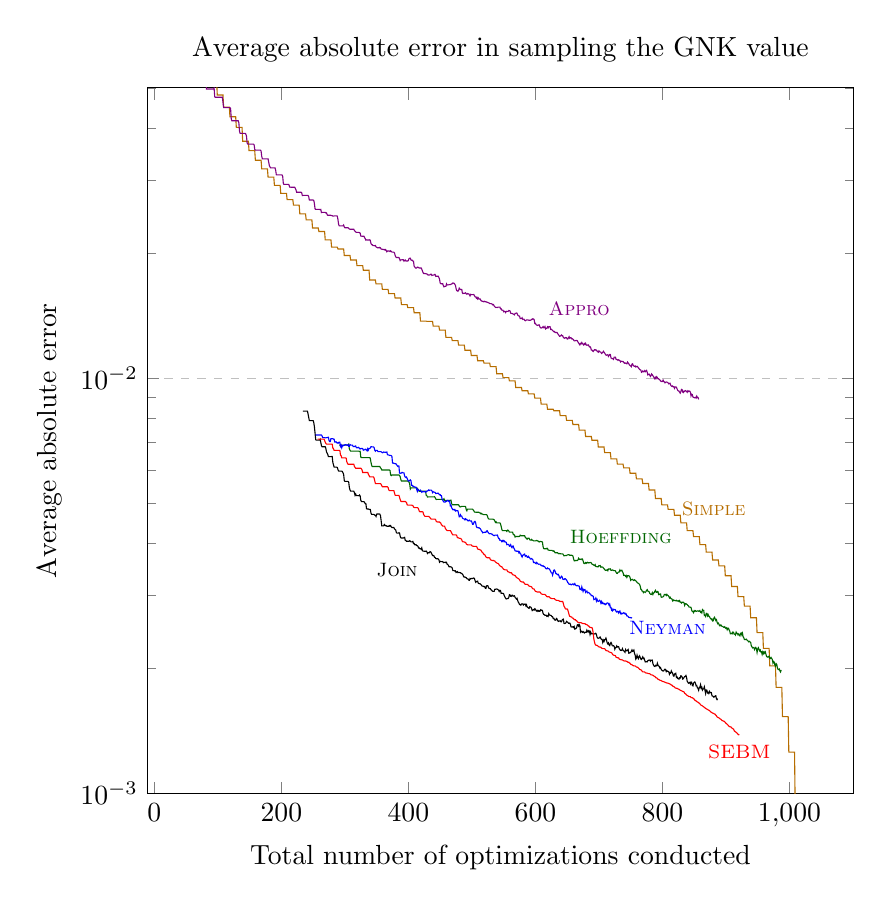
\begin{tikzpicture}
		\begin{axis}[
			title={Average absolute error in sampling the GNK value},
			xlabel={Total number of optimizations conducted},
			ylabel={Average absolute error},
			%xmin=0, xmax=0.25,
			ymin=0.001, ymax=0.05,
			ymode=log,
			%xtick={0,0.05,0.1,0.15,0.2,0.25},
			%ytick={0,20,40,60,80,100},
			%yticklabel=$\pgfmathprintnumber{\tick}\%$,
			legend pos=south west,
			ymajorgrids=true,
			grid style=dashed,
			%xticklabel style={/pgf/number format/fixed}
			width = 300,
			height = 300
		]
		\addplot[color={rgb:red,4;green,2;yellow,1}] coordinates {
(39,0.0905511314206)(40,0.0905511314206)(41,0.0905511314206)(42,0.0905511314206)(43,0.0905511314206)(44,0.0905511314206)(45,0.0905511314206)(46,0.0905511314206)(47,0.0905511314206)(48,0.0905511314206)(49,0.0800346783099)(50,0.0800346783099)(51,0.0800346783099)(52,0.0800346783099)(53,0.0800346783099)(54,0.0800346783099)(55,0.0800346783099)(56,0.0800346783099)(57,0.0800346783099)(58,0.0800346783099)(59,0.0726818288329)(60,0.0726818288329)(61,0.0726818288329)(62,0.0726818288329)(63,0.0726818288329)(64,0.0726818288329)(65,0.0726818288329)(66,0.0726818288329)(67,0.0726818288329)(68,0.0726818288329)(69,0.0639984808006)(70,0.0639984808006)(71,0.0639984808006)(72,0.0639984808006)(73,0.0639984808006)(74,0.0639984808006)(75,0.0639984808006)(76,0.0639984808006)(77,0.0639984808006)(78,0.0639984808006)(79,0.0589371626675)(80,0.0589371626675)(81,0.0589371626675)(82,0.0589371626675)(83,0.0589371626675)(84,0.0589371626675)(85,0.0589371626675)(86,0.0589371626675)(87,0.0589371626675)(88,0.0589371626675)(89,0.0520142601085)(90,0.0520142601085)(91,0.0520142601085)(92,0.0520142601085)(93,0.0520142601085)(94,0.0520142601085)(95,0.0520142601085)(96,0.0520142601085)(97,0.0520142601085)(98,0.0520142601085)(99,0.0480768858393)(100,0.0480768858393)(101,0.0480768858393)(102,0.0480768858393)(103,0.0480768858393)(104,0.0480768858393)(105,0.0480768858393)(106,0.0480768858393)(107,0.0480768858393)(108,0.0480768858393)(109,0.0449401631859)(110,0.0449401631859)(111,0.0449401631859)(112,0.0449401631859)(113,0.0449401631859)(114,0.0449401631859)(115,0.0449401631859)(116,0.0449401631859)(117,0.0449401631859)(118,0.0449401631859)(119,0.0426158587744)(120,0.0426158587744)(121,0.0426158587744)(122,0.0426158587744)(123,0.0426158587744)(124,0.0426158587744)(125,0.0426158587744)(126,0.0426158587744)(127,0.0426158587744)(128,0.0426158587744)(129,0.0401740115504)(130,0.0401740115504)(131,0.0401740115504)(132,0.0401740115504)(133,0.0401740115504)(134,0.0401740115504)(135,0.0401740115504)(136,0.0401740115504)(137,0.0401740115504)(138,0.0401740115504)(139,0.0372039977439)(140,0.0372039977439)(141,0.0372039977439)(142,0.0372039977439)(143,0.0372039977439)(144,0.0372039977439)(145,0.0372039977439)(146,0.0372039977439)(147,0.0372039977439)(148,0.0372039977439)(149,0.0353250731826)(150,0.0353250731826)(151,0.0353250731826)(152,0.0353250731826)(153,0.0353250731826)(154,0.0353250731826)(155,0.0353250731826)(156,0.0353250731826)(157,0.0353250731826)(158,0.0353250731826)(159,0.0334827529779)(160,0.0334827529779)(161,0.0334827529779)(162,0.0334827529779)(163,0.0334827529779)(164,0.0334827529779)(165,0.0334827529779)(166,0.0334827529779)(167,0.0334827529779)(168,0.0334827529779)(169,0.0319278878629)(170,0.0319278878629)(171,0.0319278878629)(172,0.0319278878629)(173,0.0319278878629)(174,0.0319278878629)(175,0.0319278878629)(176,0.0319278878629)(177,0.0319278878629)(178,0.0319278878629)(179,0.0304839904472)(180,0.0304839904472)(181,0.0304839904472)(182,0.0304839904472)(183,0.0304839904472)(184,0.0304839904472)(185,0.0304839904472)(186,0.0304839904472)(187,0.0304839904472)(188,0.0304839904472)(189,0.0291191466057)(190,0.0291191466057)(191,0.0291191466057)(192,0.0291191466057)(193,0.0291191466057)(194,0.0291191466057)(195,0.0291191466057)(196,0.0291191466057)(197,0.0291191466057)(198,0.0291191466057)(199,0.0278671669628)(200,0.0278671669628)(201,0.0278671669628)(202,0.0278671669628)(203,0.0278671669628)(204,0.0278671669628)(205,0.0278671669628)(206,0.0278671669628)(207,0.0278671669628)(208,0.0278671669628)(209,0.0269069097188)(210,0.0269069097188)(211,0.0269069097188)(212,0.0269069097188)(213,0.0269069097188)(214,0.0269069097188)(215,0.0269069097188)(216,0.0269069097188)(217,0.0269069097188)(218,0.0269069097188)(219,0.0260967155637)(220,0.0260967155637)(221,0.0260967155637)(222,0.0260967155637)(223,0.0260967155637)(224,0.0260967155637)(225,0.0260967155637)(226,0.0260967155637)(227,0.0260967155637)(228,0.0260967155637)(229,0.0248749696626)(230,0.0248749696626)(231,0.0248749696626)(232,0.0248749696626)(233,0.0248749696626)(234,0.0248749696626)(235,0.0248749696626)(236,0.0248749696626)(237,0.0248749696626)(238,0.0248749696626)(239,0.0240630795676)(240,0.0240630795676)(241,0.0240630795676)(242,0.0240630795676)(243,0.0240630795676)(244,0.0240630795676)(245,0.0240630795676)(246,0.0240630795676)(247,0.0240630795676)(248,0.0240630795676)(249,0.0229955441136)(250,0.0229955441136)(251,0.0229955441136)(252,0.0229955441136)(253,0.0229955441136)(254,0.0229955441136)(255,0.0229955441136)(256,0.0229955441136)(257,0.0229955441136)(258,0.0229955441136)(259,0.022549785203)(260,0.022549785203)(261,0.022549785203)(262,0.022549785203)(263,0.022549785203)(264,0.022549785203)(265,0.022549785203)(266,0.022549785203)(267,0.022549785203)(268,0.022549785203)(269,0.0215391100838)(270,0.0215391100838)(271,0.0215391100838)(272,0.0215391100838)(273,0.0215391100838)(274,0.0215391100838)(275,0.0215391100838)(276,0.0215391100838)(277,0.0215391100838)(278,0.0215391100838)(279,0.0206817363819)(280,0.0206817363819)(281,0.0206817363819)(282,0.0206817363819)(283,0.0206817363819)(284,0.0206817363819)(285,0.0206817363819)(286,0.0206817363819)(287,0.0206817363819)(288,0.0206817363819)(289,0.0204659089804)(290,0.0204659089804)(291,0.0204659089804)(292,0.0204659089804)(293,0.0204659089804)(294,0.0204659089804)(295,0.0204659089804)(296,0.0204659089804)(297,0.0204659089804)(298,0.0204659089804)(299,0.0197474301251)(300,0.0197474301251)(301,0.0197474301251)(302,0.0197474301251)(303,0.0197474301251)(304,0.0197474301251)(305,0.0197474301251)(306,0.0197474301251)(307,0.0197474301251)(308,0.0197474301251)(309,0.0192638138498)(310,0.0192638138498)(311,0.0192638138498)(312,0.0192638138498)(313,0.0192638138498)(314,0.0192638138498)(315,0.0192638138498)(316,0.0192638138498)(317,0.0192638138498)(318,0.0192638138498)(319,0.0186633366799)(320,0.0186633366799)(321,0.0186633366799)(322,0.0186633366799)(323,0.0186633366799)(324,0.0186633366799)(325,0.0186633366799)(326,0.0186633366799)(327,0.0186633366799)(328,0.0186633366799)(329,0.0182006027658)(330,0.0182006027658)(331,0.0182006027658)(332,0.0182006027658)(333,0.0182006027658)(334,0.0182006027658)(335,0.0182006027658)(336,0.0182006027658)(337,0.0182006027658)(338,0.0182006027658)(339,0.0172341200202)(340,0.0172341200202)(341,0.0172341200202)(342,0.0172341200202)(343,0.0172341200202)(344,0.0172341200202)(345,0.0172341200202)(346,0.0172341200202)(347,0.0172341200202)(348,0.0172341200202)(349,0.0168660464006)(350,0.0168660464006)(351,0.0168660464006)(352,0.0168660464006)(353,0.0168660464006)(354,0.0168660464006)(355,0.0168660464006)(356,0.0168660464006)(357,0.0168660464006)(358,0.0168660464006)(359,0.0163614719212)(360,0.0163614719212)(361,0.0163614719212)(362,0.0163614719212)(363,0.0163614719212)(364,0.0163614719212)(365,0.0163614719212)(366,0.0163614719212)(367,0.0163614719212)(368,0.0163614719212)(369,0.0159787483327)(370,0.0159787483327)(371,0.0159787483327)(372,0.0159787483327)(373,0.0159787483327)(374,0.0159787483327)(375,0.0159787483327)(376,0.0159787483327)(377,0.0159787483327)(378,0.0159787483327)(379,0.0155992845832)(380,0.0155992845832)(381,0.0155992845832)(382,0.0155992845832)(383,0.0155992845832)(384,0.0155992845832)(385,0.0155992845832)(386,0.0155992845832)(387,0.0155992845832)(388,0.0155992845832)(389,0.0150360607517)(390,0.0150360607517)(391,0.0150360607517)(392,0.0150360607517)(393,0.0150360607517)(394,0.0150360607517)(395,0.0150360607517)(396,0.0150360607517)(397,0.0150360607517)(398,0.0150360607517)(399,0.014787112882)(400,0.014787112882)(401,0.014787112882)(402,0.014787112882)(403,0.014787112882)(404,0.014787112882)(405,0.014787112882)(406,0.014787112882)(407,0.014787112882)(408,0.014787112882)(409,0.0143791385602)(410,0.0143791385602)(411,0.0143791385602)(412,0.0143791385602)(413,0.0143791385602)(414,0.0143791385602)(415,0.0143791385602)(416,0.0143791385602)(417,0.0143791385602)(418,0.0143791385602)(419,0.0137237284373)(420,0.0137237284373)(421,0.0137237284373)(422,0.0137237284373)(423,0.0137237284373)(424,0.0137237284373)(425,0.0137237284373)(426,0.0137237284373)(427,0.0137237284373)(428,0.0137237284373)(429,0.01370085711)(430,0.01370085711)(431,0.01370085711)(432,0.01370085711)(433,0.01370085711)(434,0.01370085711)(435,0.01370085711)(436,0.01370085711)(437,0.01370085711)(438,0.01370085711)(439,0.0133516232869)(440,0.0133516232869)(441,0.0133516232869)(442,0.0133516232869)(443,0.0133516232869)(444,0.0133516232869)(445,0.0133516232869)(446,0.0133516232869)(447,0.0133516232869)(448,0.0133516232869)(449,0.0130557105539)(450,0.0130557105539)(451,0.0130557105539)(452,0.0130557105539)(453,0.0130557105539)(454,0.0130557105539)(455,0.0130557105539)(456,0.0130557105539)(457,0.0130557105539)(458,0.0130557105539)(459,0.0125405867102)(460,0.0125405867102)(461,0.0125405867102)(462,0.0125405867102)(463,0.0125405867102)(464,0.0125405867102)(465,0.0125405867102)(466,0.0125405867102)(467,0.0125405867102)(468,0.0125405867102)(469,0.0123170987621)(470,0.0123170987621)(471,0.0123170987621)(472,0.0123170987621)(473,0.0123170987621)(474,0.0123170987621)(475,0.0123170987621)(476,0.0123170987621)(477,0.0123170987621)(478,0.0123170987621)(479,0.0120153615181)(480,0.0120153615181)(481,0.0120153615181)(482,0.0120153615181)(483,0.0120153615181)(484,0.0120153615181)(485,0.0120153615181)(486,0.0120153615181)(487,0.0120153615181)(488,0.0120153615181)(489,0.0116747189614)(490,0.0116747189614)(491,0.0116747189614)(492,0.0116747189614)(493,0.0116747189614)(494,0.0116747189614)(495,0.0116747189614)(496,0.0116747189614)(497,0.0116747189614)(498,0.0116747189614)(499,0.0113416414427)(500,0.0113416414427)(501,0.0113416414427)(502,0.0113416414427)(503,0.0113416414427)(504,0.0113416414427)(505,0.0113416414427)(506,0.0113416414427)(507,0.0113416414427)(508,0.0113416414427)(509,0.0110141470141)(510,0.0110141470141)(511,0.0110141470141)(512,0.0110141470141)(513,0.0110141470141)(514,0.0110141470141)(515,0.0110141470141)(516,0.0110141470141)(517,0.0110141470141)(518,0.0110141470141)(519,0.0108760396439)(520,0.0108760396439)(521,0.0108760396439)(522,0.0108760396439)(523,0.0108760396439)(524,0.0108760396439)(525,0.0108760396439)(526,0.0108760396439)(527,0.0108760396439)(528,0.0108760396439)(529,0.0106633858342)(530,0.0106633858342)(531,0.0106633858342)(532,0.0106633858342)(533,0.0106633858342)(534,0.0106633858342)(535,0.0106633858342)(536,0.0106633858342)(537,0.0106633858342)(538,0.0106633858342)(539,0.0102490499393)(540,0.0102490499393)(541,0.0102490499393)(542,0.0102490499393)(543,0.0102490499393)(544,0.0102490499393)(545,0.0102490499393)(546,0.0102490499393)(547,0.0102490499393)(548,0.0102490499393)(549,0.0100346175404)(550,0.0100346175404)(551,0.0100346175404)(552,0.0100346175404)(553,0.0100346175404)(554,0.0100346175404)(555,0.0100346175404)(556,0.0100346175404)(557,0.0100346175404)(558,0.0100346175404)(559,0.00985135792824)(560,0.00985135792824)(561,0.00985135792824)(562,0.00985135792824)(563,0.00985135792824)(564,0.00985135792824)(565,0.00985135792824)(566,0.00985135792824)(567,0.00985135792824)(568,0.00985135792824)(569,0.0094963232803)(570,0.0094963232803)(571,0.0094963232803)(572,0.0094963232803)(573,0.0094963232803)(574,0.0094963232803)(575,0.0094963232803)(576,0.0094963232803)(577,0.0094963232803)(578,0.0094963232803)(579,0.00932771903292)(580,0.00932771903292)(581,0.00932771903292)(582,0.00932771903292)(583,0.00932771903292)(584,0.00932771903292)(585,0.00932771903292)(586,0.00932771903292)(587,0.00932771903292)(588,0.00932771903292)(589,0.0091665256745)(590,0.0091665256745)(591,0.0091665256745)(592,0.0091665256745)(593,0.0091665256745)(594,0.0091665256745)(595,0.0091665256745)(596,0.0091665256745)(597,0.0091665256745)(598,0.0091665256745)(599,0.00895843816022)(600,0.00895843816022)(601,0.00895843816022)(602,0.00895843816022)(603,0.00895843816022)(604,0.00895843816022)(605,0.00895843816022)(606,0.00895843816022)(607,0.00895843816022)(608,0.00895843816022)(609,0.00866117603198)(610,0.00866117603198)(611,0.00866117603198)(612,0.00866117603198)(613,0.00866117603198)(614,0.00866117603198)(615,0.00866117603198)(616,0.00866117603198)(617,0.00866117603198)(618,0.00866117603198)(619,0.00842138476673)(620,0.00842138476673)(621,0.00842138476673)(622,0.00842138476673)(623,0.00842138476673)(624,0.00842138476673)(625,0.00842138476673)(626,0.00842138476673)(627,0.00842138476673)(628,0.00842138476673)(629,0.00834999234349)(630,0.00834999234349)(631,0.00834999234349)(632,0.00834999234349)(633,0.00834999234349)(634,0.00834999234349)(635,0.00834999234349)(636,0.00834999234349)(637,0.00834999234349)(638,0.00834999234349)(639,0.00812553427356)(640,0.00812553427356)(641,0.00812553427356)(642,0.00812553427356)(643,0.00812553427356)(644,0.00812553427356)(645,0.00812553427356)(646,0.00812553427356)(647,0.00812553427356)(648,0.00812553427356)(649,0.00791400443271)(650,0.00791400443271)(651,0.00791400443271)(652,0.00791400443271)(653,0.00791400443271)(654,0.00791400443271)(655,0.00791400443271)(656,0.00791400443271)(657,0.00791400443271)(658,0.00791400443271)(659,0.00773784499311)(660,0.00773784499311)(661,0.00773784499311)(662,0.00773784499311)(663,0.00773784499311)(664,0.00773784499311)(665,0.00773784499311)(666,0.00773784499311)(667,0.00773784499311)(668,0.00773784499311)(669,0.00749844299911)(670,0.00749844299911)(671,0.00749844299911)(672,0.00749844299911)(673,0.00749844299911)(674,0.00749844299911)(675,0.00749844299911)(676,0.00749844299911)(677,0.00749844299911)(678,0.00749844299911)(679,0.00724137238088)(680,0.00724137238088)(681,0.00724137238088)(682,0.00724137238088)(683,0.00724137238088)(684,0.00724137238088)(685,0.00724137238088)(686,0.00724137238088)(687,0.00724137238088)(688,0.00724137238088)(689,0.00708950769457)(690,0.00708950769457)(691,0.00708950769457)(692,0.00708950769457)(693,0.00708950769457)(694,0.00708950769457)(695,0.00708950769457)(696,0.00708950769457)(697,0.00708950769457)(698,0.00708950769457)(699,0.00682787976738)(700,0.00682787976738)(701,0.00682787976738)(702,0.00682787976738)(703,0.00682787976738)(704,0.00682787976738)(705,0.00682787976738)(706,0.00682787976738)(707,0.00682787976738)(708,0.00682787976738)(709,0.00661864066481)(710,0.00661864066481)(711,0.00661864066481)(712,0.00661864066481)(713,0.00661864066481)(714,0.00661864066481)(715,0.00661864066481)(716,0.00661864066481)(717,0.00661864066481)(718,0.00661864066481)(719,0.00639364102019)(720,0.00639364102019)(721,0.00639364102019)(722,0.00639364102019)(723,0.00639364102019)(724,0.00639364102019)(725,0.00639364102019)(726,0.00639364102019)(727,0.00639364102019)(728,0.00639364102019)(729,0.00621096032214)(730,0.00621096032214)(731,0.00621096032214)(732,0.00621096032214)(733,0.00621096032214)(734,0.00621096032214)(735,0.00621096032214)(736,0.00621096032214)(737,0.00621096032214)(738,0.00621096032214)(739,0.00608479948542)(740,0.00608479948542)(741,0.00608479948542)(742,0.00608479948542)(743,0.00608479948542)(744,0.00608479948542)(745,0.00608479948542)(746,0.00608479948542)(747,0.00608479948542)(748,0.00608479948542)(749,0.0059062874642)(750,0.0059062874642)(751,0.0059062874642)(752,0.0059062874642)(753,0.0059062874642)(754,0.0059062874642)(755,0.0059062874642)(756,0.0059062874642)(757,0.0059062874642)(758,0.0059062874642)(759,0.00572317006733)(760,0.00572317006733)(761,0.00572317006733)(762,0.00572317006733)(763,0.00572317006733)(764,0.00572317006733)(765,0.00572317006733)(766,0.00572317006733)(767,0.00572317006733)(768,0.00572317006733)(769,0.00557713588006)(770,0.00557713588006)(771,0.00557713588006)(772,0.00557713588006)(773,0.00557713588006)(774,0.00557713588006)(775,0.00557713588006)(776,0.00557713588006)(777,0.00557713588006)(778,0.00557713588006)(779,0.00538203943173)(780,0.00538203943173)(781,0.00538203943173)(782,0.00538203943173)(783,0.00538203943173)(784,0.00538203943173)(785,0.00538203943173)(786,0.00538203943173)(787,0.00538203943173)(788,0.00538203943173)(789,0.00513450895927)(790,0.00513450895927)(791,0.00513450895927)(792,0.00513450895927)(793,0.00513450895927)(794,0.00513450895927)(795,0.00513450895927)(796,0.00513450895927)(797,0.00513450895927)(798,0.00513450895927)(799,0.00495552378235)(800,0.00495552378235)(801,0.00495552378235)(802,0.00495552378235)(803,0.00495552378235)(804,0.00495552378235)(805,0.00495552378235)(806,0.00495552378235)(807,0.00495552378235)(808,0.00495552378235)(809,0.00483390372303)(810,0.00483390372303)(811,0.00483390372303)(812,0.00483390372303)(813,0.00483390372303)(814,0.00483390372303)(815,0.00483390372303)(816,0.00483390372303)(817,0.00483390372303)(818,0.00483390372303)(819,0.00467825266765)(820,0.00467825266765)(821,0.00467825266765)(822,0.00467825266765)(823,0.00467825266765)(824,0.00467825266765)(825,0.00467825266765)(826,0.00467825266765)(827,0.00467825266765)(828,0.00467825266765)(829,0.0044834768048)(830,0.0044834768048)(831,0.0044834768048)(832,0.0044834768048)(833,0.0044834768048)(834,0.0044834768048)(835,0.0044834768048)(836,0.0044834768048)(837,0.0044834768048)(838,0.0044834768048)(839,0.00429503523792)(840,0.00429503523792)(841,0.00429503523792)(842,0.00429503523792)(843,0.00429503523792)(844,0.00429503523792)(845,0.00429503523792)(846,0.00429503523792)(847,0.00429503523792)(848,0.00429503523792)(849,0.00415707615011)(850,0.00415707615011)(851,0.00415707615011)(852,0.00415707615011)(853,0.00415707615011)(854,0.00415707615011)(855,0.00415707615011)(856,0.00415707615011)(857,0.00415707615011)(858,0.00415707615011)(859,0.00397706635755)(860,0.00397706635755)(861,0.00397706635755)(862,0.00397706635755)(863,0.00397706635755)(864,0.00397706635755)(865,0.00397706635755)(866,0.00397706635755)(867,0.00397706635755)(868,0.00397706635755)(869,0.00381281348984)(870,0.00381281348984)(871,0.00381281348984)(872,0.00381281348984)(873,0.00381281348984)(874,0.00381281348984)(875,0.00381281348984)(876,0.00381281348984)(877,0.00381281348984)(878,0.00381281348984)(879,0.00364990819327)(880,0.00364990819327)(881,0.00364990819327)(882,0.00364990819327)(883,0.00364990819327)(884,0.00364990819327)(885,0.00364990819327)(886,0.00364990819327)(887,0.00364990819327)(888,0.00364990819327)(889,0.00353431032454)(890,0.00353431032454)(891,0.00353431032454)(892,0.00353431032454)(893,0.00353431032454)(894,0.00353431032454)(895,0.00353431032454)(896,0.00353431032454)(897,0.00353431032454)(898,0.00353431032454)(899,0.00334558007011)(900,0.00334558007011)(901,0.00334558007011)(902,0.00334558007011)(903,0.00334558007011)(904,0.00334558007011)(905,0.00334558007011)(906,0.00334558007011)(907,0.00334558007011)(908,0.00334558007011)(909,0.00315243863112)(910,0.00315243863112)(911,0.00315243863112)(912,0.00315243863112)(913,0.00315243863112)(914,0.00315243863112)(915,0.00315243863112)(916,0.00315243863112)(917,0.00315243863112)(918,0.00315243863112)(919,0.00298012814551)(920,0.00298012814551)(921,0.00298012814551)(922,0.00298012814551)(923,0.00298012814551)(924,0.00298012814551)(925,0.00298012814551)(926,0.00298012814551)(927,0.00298012814551)(928,0.00298012814551)(929,0.00282644981654)(930,0.00282644981654)(931,0.00282644981654)(932,0.00282644981654)(933,0.00282644981654)(934,0.00282644981654)(935,0.00282644981654)(936,0.00282644981654)(937,0.00282644981654)(938,0.00282644981654)(939,0.00265057632368)(940,0.00265057632368)(941,0.00265057632368)(942,0.00265057632368)(943,0.00265057632368)(944,0.00265057632368)(945,0.00265057632368)(946,0.00265057632368)(947,0.00265057632368)(948,0.00265057632368)(949,0.0024398130575)(950,0.0024398130575)(951,0.0024398130575)(952,0.0024398130575)(953,0.0024398130575)(954,0.0024398130575)(955,0.0024398130575)(956,0.0024398130575)(957,0.0024398130575)(958,0.0024398130575)(959,0.00223672487232)(960,0.00223672487232)(961,0.00223672487232)(962,0.00223672487232)(963,0.00223672487232)(964,0.00223672487232)(965,0.00223672487232)(966,0.00223672487232)(967,0.00223672487232)(968,0.00223672487232)(969,0.00203027235392)(970,0.00203027235392)(971,0.00203027235392)(972,0.00203027235392)(973,0.00203027235392)(974,0.00203027235392)(975,0.00203027235392)(976,0.00203027235392)(977,0.00203027235392)(978,0.00203027235392)(979,0.00180169313843)(980,0.00180169313843)(981,0.00180169313843)(982,0.00180169313843)(983,0.00180169313843)(984,0.00180169313843)(985,0.00180169313843)(986,0.00180169313843)(987,0.00180169313843)(988,0.00180169313843)(989,0.00153191939809)(990,0.00153191939809)(991,0.00153191939809)(992,0.00153191939809)(993,0.00153191939809)(994,0.00153191939809)(995,0.00153191939809)(996,0.00153191939809)(997,0.00153191939809)(998,0.00153191939809)(999,0.00125809095339)(1000,0.00125809095339)(1001,0.00125809095339)(1002,0.00125809095339)(1003,0.00125809095339)(1004,0.00125809095339)(1005,0.00125809095339)(1006,0.00125809095339)(1007,0.00125809095339)(1008,0.00125809095339)(1009,0.000933425005574)
			}node[pos=0.8](endofplotsquare){} ;
		\node [right,color={rgb:red,4;green,2;yellow,1}] at (endofplotsquare) {\scriptsize \textsc{Simple}};
		\addplot[] coordinates {
(234,0.00833467354893)(235,0.00833467354893)(236,0.00833467354893)(237,0.00833467354893)(238,0.00833467354893)(239,0.00833467354893)(240,0.00833467354893)(241,0.00833467354893)(242,0.00819416201223)(243,0.00804637411033)(244,0.00790760630473)(245,0.00790760630473)(246,0.00790760630473)(247,0.00790760630473)(248,0.00790760630473)(249,0.00790760630473)(250,0.00790760630473)(251,0.00781595878001)(252,0.00762932274038)(253,0.00737468339388)(254,0.00711395952161)(255,0.00709575962179)(256,0.00709575962179)(257,0.00709575962179)(258,0.00709575962179)(259,0.00709575962179)(260,0.00709575962179)(261,0.00712912125074)(262,0.00701115736292)(263,0.00687924118469)(264,0.00684115991267)(265,0.00684115991267)(266,0.00684115991267)(267,0.00684115991267)(268,0.00684115991267)(269,0.00684115991267)(270,0.0067740043007)(271,0.00664348229147)(272,0.00660705611431)(273,0.00655327781385)(274,0.00647584340558)(275,0.00647584340558)(276,0.00647584340558)(277,0.00647584340558)(278,0.00647584340558)(279,0.00647827891478)(280,0.00647827891478)(281,0.00626460364134)(282,0.00618885388644)(283,0.00611092382737)(284,0.00611092382737)(285,0.00611092382737)(286,0.00611092382737)(287,0.00611092382737)(288,0.00609383025141)(289,0.00602804291619)(290,0.00597952451459)(291,0.00597605143157)(292,0.00597605143157)(293,0.00597605143157)(294,0.00597605143157)(295,0.00597605143157)(296,0.00596089385111)(297,0.00592002450658)(298,0.00586617847968)(299,0.00567450304149)(300,0.00564384705448)(301,0.00564384705448)(302,0.00564384705448)(303,0.00564384705448)(304,0.00564384705448)(305,0.00564384705448)(306,0.00561752883891)(307,0.00545571976476)(308,0.00538310802782)(309,0.00534676141769)(310,0.00534676141769)(311,0.00534676141769)(312,0.00534676141769)(313,0.00534676141769)(314,0.00534676141769)(315,0.00529915791441)(316,0.00522364165276)(317,0.00525917690617)(318,0.00521698132363)(319,0.00521698132363)(320,0.00521698132363)(321,0.00521698132363)(322,0.00521167015101)(323,0.00523369095712)(324,0.0052090086909)(325,0.00508425841782)(326,0.00504677915584)(327,0.00504677915584)(328,0.00504677915584)(329,0.00504677915584)(330,0.00504677915584)(331,0.00501760465129)(332,0.00499275961414)(333,0.00498879678946)(334,0.00485081489746)(335,0.0048439417019)(336,0.0048439417019)(337,0.0048439417019)(338,0.0048342041735)(339,0.0048342041735)(340,0.00482959886062)(341,0.00473897706952)(342,0.00470041600234)(343,0.00470041600234)(344,0.00470041600234)(345,0.00470041600234)(346,0.00469655944263)(347,0.00467990095362)(348,0.00467506918242)(349,0.00464679646119)(350,0.00470798526707)(351,0.00471152645251)(352,0.00471152645251)(353,0.00471152645251)(354,0.00471152645251)(355,0.00470719504718)(356,0.00466892969711)(357,0.0045480266176)(358,0.00441161218531)(359,0.00441161218531)(360,0.00441161218531)(361,0.00441161218531)(362,0.00444503771652)(363,0.00442695179011)(364,0.00441383222604)(365,0.00441491261519)(366,0.00440136241673)(367,0.00440136241673)(368,0.00440136241673)(369,0.00440136241673)(370,0.00441890792289)(371,0.00440659988465)(372,0.00441857399724)(373,0.00438401136772)(374,0.00437189095833)(375,0.00437189095833)(376,0.00437189095833)(377,0.00437189095833)(378,0.00434072734956)(379,0.00432212833332)(380,0.00431291657158)(381,0.00425000411553)(382,0.00423664808147)(383,0.00423664808147)(384,0.00423664808147)(385,0.00424495850705)(386,0.00424017498042)(387,0.00416877864414)(388,0.00412700957878)(389,0.00412419818817)(390,0.00412419818817)(391,0.00412419818817)(392,0.00412419818817)(393,0.00413177582817)(394,0.00413933034399)(395,0.00407019302416)(396,0.00406636920464)(397,0.00404938122422)(398,0.00404938122422)(399,0.00404938122422)(400,0.00404938122422)(401,0.00404703949314)(402,0.00406349644449)(403,0.00405176927034)(404,0.00403614756276)(405,0.00403614756276)(406,0.00403614756276)(407,0.004046577306)(408,0.00399843580623)(409,0.00400071149455)(410,0.0039740039064)(411,0.0039740039064)(412,0.0039740039064)(413,0.0039554319733)(414,0.00395374838292)(415,0.0039395750328)(416,0.00390168643245)(417,0.00390497327368)(418,0.0038855294032)(419,0.0038855294032)(420,0.00387554213629)(421,0.00390573275061)(422,0.00384635580636)(423,0.00383550259511)(424,0.00383550259511)(425,0.00383140654688)(426,0.00383164197875)(427,0.00383164197875)(428,0.00383614716313)(429,0.00382028765538)(430,0.00378586719064)(431,0.00380199256804)(432,0.00380199256804)(433,0.00380199256804)(434,0.00382530338898)(435,0.00382048566972)(436,0.00379732359055)(437,0.00377289415239)(438,0.00374297057207)(439,0.00374259966267)(440,0.00374106242248)(441,0.00370621334134)(442,0.00370220827722)(443,0.00368175101647)(444,0.003676079299)(445,0.003676079299)(446,0.003676079299)(447,0.0036709426275)(448,0.00365476219629)(449,0.00360805026142)(450,0.00362471716342)(451,0.00361932845704)(452,0.00361932845704)(453,0.00361901180381)(454,0.00361963565818)(455,0.0035981450841)(456,0.00360235046357)(457,0.00360235046357)(458,0.00360785251023)(459,0.00359480156182)(460,0.00360389525204)(461,0.00356568862031)(462,0.00355754047682)(463,0.00354423885585)(464,0.00351747478195)(465,0.00351747478195)(466,0.00351747478195)(467,0.00351362044631)(468,0.00350726174241)(469,0.00349135008802)(470,0.00344171405358)(471,0.00344182861025)(472,0.00344182861025)(473,0.00343410096894)(474,0.00343888057968)(475,0.00340708688267)(476,0.00341717489421)(477,0.00342371192911)(478,0.00340405135661)(479,0.00340902988078)(480,0.00340634220067)(481,0.00340320129486)(482,0.00340404916671)(483,0.00338932730354)(484,0.00338899041948)(485,0.00337361758514)(486,0.00335972954794)(487,0.00332491206341)(488,0.0033223389364)(489,0.0033223389364)(490,0.00331275816714)(491,0.0033109972032)(492,0.00329299449864)(493,0.00328737870801)(494,0.00328518171428)(495,0.00326568295163)(496,0.00326155046451)(497,0.00329520697908)(498,0.00328732800631)(499,0.00329467338016)(500,0.00329467338016)(501,0.00329472869399)(502,0.00329981363714)(503,0.00330488848667)(504,0.00329333361508)(505,0.00325332288526)(506,0.00322680281345)(507,0.00324121987381)(508,0.00323983834737)(509,0.00324616133679)(510,0.00321024210076)(511,0.00320460094098)(512,0.00320025913361)(513,0.00320070509512)(514,0.00318746303673)(515,0.00317785282062)(516,0.00315810893213)(517,0.00315887036541)(518,0.00315569979525)(519,0.00314844047522)(520,0.00315198196609)(521,0.00312209346027)(522,0.00311830960163)(523,0.00316392218256)(524,0.00316669674134)(525,0.00316562167622)(526,0.00313965385037)(527,0.00311818865056)(528,0.00311488427857)(529,0.00311488427857)(530,0.00309538848896)(531,0.00309018754039)(532,0.00307169199701)(533,0.00306898188693)(534,0.00306861671563)(535,0.00306861671563)(536,0.00310339491709)(537,0.00310394528438)(538,0.00310678590885)(539,0.00310876448861)(540,0.00310616787302)(541,0.00309749520559)(542,0.00308827250453)(543,0.00306576956414)(544,0.00308639804942)(545,0.00308099524238)(546,0.00303506313225)(547,0.00303811939846)(548,0.00303482270992)(549,0.00303482270992)(550,0.00302610080609)(551,0.0029933780466)(552,0.00297447657098)(553,0.00295314697578)(554,0.00294159052865)(555,0.00294393672872)(556,0.00294829273811)(557,0.00294829186524)(558,0.00296476050034)(559,0.00301262709219)(560,0.00300982771615)(561,0.00298601084288)(562,0.00298364631692)(563,0.00300211360009)(564,0.00300211360009)(565,0.00298657973186)(566,0.00298991227236)(567,0.0029938479985)(568,0.00296611866599)(569,0.00295638732281)(570,0.00294071208171)(571,0.00295220787717)(572,0.00291968652445)(573,0.00288994063915)(574,0.0028756661691)(575,0.00285178285163)(576,0.00285252251492)(577,0.00284243938081)(578,0.0028581481661)(579,0.00286341978634)(580,0.00285925654449)(581,0.00284342562774)(582,0.002858955291)(583,0.00285483346381)(584,0.00285811769103)(585,0.00283133349662)(586,0.00284805703216)(587,0.0028126252231)(588,0.00280786475208)(589,0.00279798357848)(590,0.00279250076808)(591,0.00281863150109)(592,0.0028140647608)(593,0.00280859330047)(594,0.00278765518495)(595,0.00275781690458)(596,0.00276509260247)(597,0.00277403006238)(598,0.00276595582821)(599,0.00278711179809)(600,0.00277981610031)(601,0.00275745187585)(602,0.00275005175423)(603,0.0027606577132)(604,0.00274604871276)(605,0.00275860480917)(606,0.00274798754005)(607,0.00274616584557)(608,0.00276987963025)(609,0.00276205348322)(610,0.00276585119227)(611,0.00275918670011)(612,0.00271544609034)(613,0.00269957001727)(614,0.00269457136466)(615,0.00268526645538)(616,0.00268833045423)(617,0.00268719303171)(618,0.00267173196651)(619,0.00267878679611)(620,0.00267049559154)(621,0.00271199876541)(622,0.00269344408522)(623,0.00268577418851)(624,0.00268689115172)(625,0.00268185351438)(626,0.00266632247966)(627,0.00266525872883)(628,0.00263873970164)(629,0.00264123108196)(630,0.00262216039196)(631,0.0026136211837)(632,0.00261633574921)(633,0.00264048428254)(634,0.00263188742159)(635,0.00260990894675)(636,0.0025970359405)(637,0.00260310706281)(638,0.0026018784123)(639,0.0026061466671)(640,0.00259233412465)(641,0.00259115210669)(642,0.00261770275849)(643,0.00262714659502)(644,0.00263066201076)(645,0.00256938874994)(646,0.0025669407018)(647,0.00256944476749)(648,0.00257649221125)(649,0.00259743642388)(650,0.00258992649488)(651,0.00258448612051)(652,0.00257111759122)(653,0.00257022775609)(654,0.00257377050887)(655,0.00255841707576)(656,0.00252138162806)(657,0.00251847579735)(658,0.00251628386548)(659,0.0025225089143)(660,0.00251132531962)(661,0.00252413663172)(662,0.0024884745011)(663,0.00249228075837)(664,0.00249682006476)(665,0.00251214405402)(666,0.00254750538397)(667,0.00255092474094)(668,0.0025318759044)(669,0.00255273793174)(670,0.00253708385937)(671,0.00244786298644)(672,0.00246059964413)(673,0.0024517950406)(674,0.00244454450685)(675,0.00245624780398)(676,0.00244519990497)(677,0.00243594293504)(678,0.00244589905196)(679,0.00244370705138)(680,0.00244340838391)(681,0.00247412898045)(682,0.0024565168481)(683,0.00244735082405)(684,0.00246810680208)(685,0.00246250278844)(686,0.00241545523592)(687,0.00244821230025)(688,0.00242507627726)(689,0.00242586648137)(690,0.0024244240503)(691,0.00242673991268)(692,0.00242530865365)(693,0.00242287189111)(694,0.00242589566379)(695,0.00243165418958)(696,0.00241578654767)(697,0.00238107102739)(698,0.00236672568806)(699,0.00236662753351)(700,0.00236575836027)(701,0.00237923533492)(702,0.00238260725478)(703,0.00236187237974)(704,0.00235080378179)(705,0.0023514747394)(706,0.00231296985072)(707,0.00234075948383)(708,0.00232381924388)(709,0.00234714077212)(710,0.00234911202963)(711,0.00236751861534)(712,0.00233889730543)(713,0.00230590656145)(714,0.002292700633)(715,0.00230542682497)(716,0.00227914331765)(717,0.00227155185692)(718,0.00229972696518)(719,0.00231162837109)(720,0.00229457058866)(721,0.00226970903008)(722,0.00226750496134)(723,0.00227085401506)(724,0.00226256938611)(725,0.00222596110969)(726,0.00224445039711)(727,0.00224755074869)(728,0.00226763683998)(729,0.00225360853043)(730,0.00225790157036)(731,0.00225854823433)(732,0.00223292949263)(733,0.00222124528073)(734,0.00221281337756)(735,0.0022112586387)(736,0.00221538754747)(737,0.00223297848262)(738,0.00221149359081)(739,0.00220683564458)(740,0.00219999176261)(741,0.00218808266064)(742,0.00222174518724)(743,0.00220585011993)(744,0.00220644040788)(745,0.00221473942163)(746,0.00222303868922)(747,0.00217742765036)(748,0.00217904761153)(749,0.00218444986116)(750,0.00218564200443)(751,0.00220140367847)(752,0.00221823728373)(753,0.00219971618962)(754,0.0022025961676)(755,0.00221542148287)(756,0.00217451068501)(757,0.00215520429111)(758,0.00210755945324)(759,0.00211881916193)(760,0.0021545593662)(761,0.00212937428091)(762,0.00211307144429)(763,0.00213643287129)(764,0.00214676968935)(765,0.0021252103818)(766,0.00210688499939)(767,0.00210301951942)(768,0.00212045844811)(769,0.00213415061395)(770,0.00211380106552)(771,0.00211791013776)(772,0.00209483856127)(773,0.00207436549072)(774,0.00207613587251)(775,0.00207852576029)(776,0.00207558556094)(777,0.00208926598577)(778,0.00209316878624)(779,0.00209663277771)(780,0.00209506265499)(781,0.00208304965506)(782,0.00209586855144)(783,0.00209303885052)(784,0.00209590912583)(785,0.00205489755984)(786,0.00203755369884)(787,0.0020261492058)(788,0.00202250457479)(789,0.00203516652643)(790,0.00202889788003)(791,0.00202963390332)(792,0.00205983077355)(793,0.00203702176183)(794,0.00202762869876)(795,0.00202452126955)(796,0.0020040502297)(797,0.00201008000522)(798,0.00199239622235)(799,0.0019815782212)(800,0.0019783873177)(801,0.00197263952259)(802,0.00197411061239)(803,0.00198722838516)(804,0.00199432377933)(805,0.00198844418604)(806,0.00196646512145)(807,0.0019765355327)(808,0.00197029451141)(809,0.00196928933186)(810,0.00196609310125)(811,0.00193785550859)(812,0.00195296908835)(813,0.00194995887869)(814,0.00197408196506)(815,0.00195808761791)(816,0.00195149170724)(817,0.00192261287835)(818,0.00191721653071)(819,0.00193837554922)(820,0.0019447872837)(821,0.00194915779242)(822,0.00190443969863)(823,0.00190878993711)(824,0.00189289504584)(825,0.00189492660773)(826,0.00188622828189)(827,0.00190175027255)(828,0.00189764944459)(829,0.00192096325165)(830,0.0019191919387)(831,0.00190810880368)(832,0.00188680090573)(833,0.00189172536897)(834,0.00190405604393)(835,0.00191343677595)(836,0.00191446516574)(837,0.0019244136297)(838,0.00190277600121)(839,0.00186429759885)(840,0.00185355958743)(841,0.00184353066067)(842,0.00184789096747)(843,0.0018521613032)(844,0.00183621322192)(845,0.00185662336)(846,0.00185464024848)(847,0.00182303788185)(848,0.00181679095326)(849,0.00184483731465)(850,0.00185145180542)(851,0.00185732318827)(852,0.00184438361009)(853,0.00181742042341)(854,0.00182050951564)(855,0.00179711280601)(856,0.00179211938253)(857,0.00177389867736)(858,0.00180279396504)(859,0.00180145854921)(860,0.00182801750149)(861,0.00179364519376)(862,0.00180370256194)(863,0.00177565218166)(864,0.0017863385721)(865,0.00178852392917)(866,0.00180746980683)(867,0.00177079367448)(868,0.00174197174743)(869,0.00177616175985)(870,0.00177395864585)(871,0.00174717387356)(872,0.00175217420595)(873,0.00174204842227)(874,0.00176215049193)(875,0.00174961116872)(876,0.00175268903431)(877,0.00174989566087)(878,0.00171979748761)(879,0.00171808119388)(880,0.00171312844776)(881,0.00170560862685)(882,0.0017127320707)(883,0.00171868120396)(884,0.00172059455618)(885,0.00169220935799)(886,0.00168321667854)(887,0.00169317098998)
			}node[pos=0.3](endofplotsquare){} ;
		\node [below left] at (endofplotsquare) {\scriptsize \textsc{Join}};
		\addplot[color=black!60!green] coordinates {
(291,0.00690172230249)(292,0.00689964028367)(293,0.00689964028367)(294,0.00689964028367)(295,0.00689964028367)(296,0.00689964028367)(297,0.00689964028367)(298,0.00689964028367)(299,0.00689964028367)(300,0.00689964028367)(301,0.00689964028367)(302,0.00689964028367)(303,0.00689964028367)(304,0.00689964028367)(305,0.00689964028367)(306,0.00693479949728)(307,0.0067586513306)(308,0.00670732279253)(309,0.00667477108082)(310,0.00667477108082)(311,0.00667477108082)(312,0.00667477108082)(313,0.00667477108082)(314,0.00667477108082)(315,0.00667477108082)(316,0.00667477108082)(317,0.00667477108082)(318,0.00667477108082)(319,0.00667477108082)(320,0.00667477108082)(321,0.00667477108082)(322,0.00667477108082)(323,0.00666664559936)(324,0.00666976099895)(325,0.00645841465978)(326,0.0064374553039)(327,0.0064374553039)(328,0.0064374553039)(329,0.0064374553039)(330,0.0064374553039)(331,0.0064374553039)(332,0.0064374553039)(333,0.0064374553039)(334,0.0064374553039)(335,0.0064374553039)(336,0.0064374553039)(337,0.0064374553039)(338,0.0064374553039)(339,0.0064374553039)(340,0.00641394699826)(341,0.00628166277487)(342,0.0061760497925)(343,0.00613052123169)(344,0.00613052123169)(345,0.00613052123169)(346,0.00613052123169)(347,0.00613052123169)(348,0.00613052123169)(349,0.00613052123169)(350,0.00613052123169)(351,0.00613052123169)(352,0.00613052123169)(353,0.00613052123169)(354,0.00613052123169)(355,0.00613052123169)(356,0.00608532875329)(357,0.00606273830125)(358,0.00601378925978)(359,0.00601378925978)(360,0.00601378925978)(361,0.00601378925978)(362,0.00601378925978)(363,0.00601378925978)(364,0.00601378925978)(365,0.00601378925978)(366,0.00601378925978)(367,0.00601378925978)(368,0.00601378925978)(369,0.00601378925978)(370,0.00601378925978)(371,0.00599588922001)(372,0.00585259046861)(373,0.00582890936594)(374,0.00584898622753)(375,0.00584898622753)(376,0.00584898622753)(377,0.00584898622753)(378,0.00584898622753)(379,0.00584898622753)(380,0.00584898622753)(381,0.00584898622753)(382,0.00584898622753)(383,0.00584898622753)(384,0.00584898622753)(385,0.00584898622753)(386,0.00583461318563)(387,0.00579554620904)(388,0.00570800349522)(389,0.0056572696049)(390,0.0056572696049)(391,0.0056572696049)(392,0.0056572696049)(393,0.0056572696049)(394,0.0056572696049)(395,0.0056572696049)(396,0.0056572696049)(397,0.0056572696049)(398,0.0056572696049)(399,0.0056572696049)(400,0.00563931048158)(401,0.00562239970595)(402,0.00556891504832)(403,0.0054120934001)(404,0.00544661039645)(405,0.00544661039645)(406,0.00544661039645)(407,0.00544661039645)(408,0.00544661039645)(409,0.00544661039645)(410,0.00544661039645)(411,0.00544661039645)(412,0.00544661039645)(413,0.00544661039645)(414,0.00543496644135)(415,0.00540055020572)(416,0.00537705161593)(417,0.00534248443944)(418,0.00534454849625)(419,0.00534454849625)(420,0.00534454849625)(421,0.00534454849625)(422,0.00534454849625)(423,0.00534454849625)(424,0.00534454849625)(425,0.00534454849625)(426,0.00534454849625)(427,0.00534454849625)(428,0.00522589617009)(429,0.00521482975425)(430,0.00517750723252)(431,0.00517812152897)(432,0.00517812152897)(433,0.00517812152897)(434,0.00517812152897)(435,0.00517812152897)(436,0.00517812152897)(437,0.00517812152897)(438,0.00517812152897)(439,0.00517812152897)(440,0.00517812152897)(441,0.00518593068988)(442,0.00516129213047)(443,0.00512025530503)(444,0.00510615531755)(445,0.00510753133254)(446,0.00510753133254)(447,0.00510753133254)(448,0.00510753133254)(449,0.00510753133254)(450,0.00510753133254)(451,0.00510753133254)(452,0.00510753133254)(453,0.00510753133254)(454,0.00510790557575)(455,0.00510173545602)(456,0.00512614435768)(457,0.00508027438807)(458,0.00508027438807)(459,0.00508027438807)(460,0.00508027438807)(461,0.00508027438807)(462,0.00508027438807)(463,0.00508027438807)(464,0.00508027438807)(465,0.00508027438807)(466,0.00508604567223)(467,0.00508821150883)(468,0.00499416365952)(469,0.00495911794689)(470,0.00495911794689)(471,0.00495911794689)(472,0.00495911794689)(473,0.00495911794689)(474,0.00495911794689)(475,0.00495911794689)(476,0.00495911794689)(477,0.00495911794689)(478,0.00495911794689)(479,0.00495708248363)(480,0.00492533394976)(481,0.00490204416062)(482,0.00489797757908)(483,0.00490994313633)(484,0.00491447545373)(485,0.00491447545373)(486,0.00491447545373)(487,0.00491447545373)(488,0.00491447545373)(489,0.00491447545373)(490,0.00490973882072)(491,0.00482436595764)(492,0.00479581279939)(493,0.00483981241354)(494,0.00483981241354)(495,0.00483981241354)(496,0.00483981241354)(497,0.00483981241354)(498,0.00483981241354)(499,0.00483981241354)(500,0.00483981241354)(501,0.00483981241354)(502,0.00481768530974)(503,0.0047952131557)(504,0.00476232038685)(505,0.00476139424825)(506,0.004758032176)(507,0.004758032176)(508,0.004758032176)(509,0.004758032176)(510,0.004758032176)(511,0.004758032176)(512,0.00474072317426)(513,0.00474072317426)(514,0.00471653693251)(515,0.00472719565213)(516,0.00470636763936)(517,0.00470636763936)(518,0.00469549942765)(519,0.00469549942765)(520,0.00469549942765)(521,0.00469549942765)(522,0.00469549942765)(523,0.0046923485157)(524,0.00467875298421)(525,0.00462327793118)(526,0.00458981587708)(527,0.00457961917382)(528,0.00457961917382)(529,0.00457961917382)(530,0.00457961917382)(531,0.00457961917382)(532,0.00457961917382)(533,0.00458014813749)(534,0.00457121746474)(535,0.00456281660917)(536,0.0045323234093)(537,0.00449678991168)(538,0.00451264762767)(539,0.00448400662407)(540,0.00448400662407)(541,0.00448400662407)(542,0.00448400662407)(543,0.00448400662407)(544,0.00448400662407)(545,0.00446126371183)(546,0.00440056713782)(547,0.00433124681623)(548,0.00429606335787)(549,0.00429606335787)(550,0.00429606335787)(551,0.00429606335787)(552,0.00429606335787)(553,0.00429606335787)(554,0.00429606335787)(555,0.00427742876435)(556,0.00430902841136)(557,0.00430523357295)(558,0.00429124895177)(559,0.00426027371865)(560,0.00426061248503)(561,0.00426061248503)(562,0.00426061248503)(563,0.00426061248503)(564,0.00426061248503)(565,0.00421211104174)(566,0.00419683701983)(567,0.0041933557003)(568,0.00414542608543)(569,0.00415885305387)(570,0.00415885305387)(571,0.00415885305387)(572,0.00415885305387)(573,0.00415885305387)(574,0.00415885305387)(575,0.00416020753909)(576,0.00419034697487)(577,0.00418347779243)(578,0.00417546946501)(579,0.00417496161501)(580,0.00417496161501)(581,0.00417496161501)(582,0.00417496161501)(583,0.00417678869805)(584,0.00413963456875)(585,0.00412741949784)(586,0.00410679248014)(587,0.00409603141745)(588,0.00411835306355)(589,0.00411835306355)(590,0.00411835306355)(591,0.00408080631803)(592,0.00408080631803)(593,0.00407377103382)(594,0.00409206735293)(595,0.00407732555055)(596,0.00407048415708)(597,0.00406008152609)(598,0.00406008152609)(599,0.00406008152609)(600,0.00406008152609)(601,0.00406124418974)(602,0.00406990301747)(603,0.00406281914211)(604,0.00405696237573)(605,0.00404234547393)(606,0.00403461620602)(607,0.00404369349141)(608,0.00404369349141)(609,0.00404369349141)(610,0.00403892125457)(611,0.00403400537024)(612,0.00393468773966)(613,0.00388744061247)(614,0.0038865909995)(615,0.0038865909995)(616,0.0038865909995)(617,0.00388330748243)(618,0.00389794454923)(619,0.00389463179728)(620,0.00385686626376)(621,0.00385628498612)(622,0.00385093492863)(623,0.00385093492863)(624,0.00385093492863)(625,0.00385093492863)(626,0.00385093492863)(627,0.00383978013047)(628,0.00383313669087)(629,0.00384102920438)(630,0.00382223077536)(631,0.00379939503268)(632,0.00379939503268)(633,0.00379939503268)(634,0.00379939503268)(635,0.00379939503268)(636,0.00378301869921)(637,0.00377855822723)(638,0.00378492880051)(639,0.00378094877223)(640,0.00377849363833)(641,0.00377849363833)(642,0.00377849363833)(643,0.00377795291001)(644,0.00375825232267)(645,0.00373589508549)(646,0.00374041008602)(647,0.00374303857149)(648,0.00374133387341)(649,0.00374133387341)(650,0.00375550073049)(651,0.00375758665574)(652,0.00375849119365)(653,0.00376045265225)(654,0.00374608340145)(655,0.00374868467065)(656,0.00374868467065)(657,0.00374868467065)(658,0.00374375139744)(659,0.00373436211341)(660,0.00367909364613)(661,0.00363549957959)(662,0.00363188053324)(663,0.0036406582782)(664,0.0036406582782)(665,0.0036406582782)(666,0.0036406582782)(667,0.00365327271046)(668,0.00368692752977)(669,0.00366687187505)(670,0.00366687187505)(671,0.00366687187505)(672,0.00365957530862)(673,0.00367347753088)(674,0.00367084605405)(675,0.00363705492826)(676,0.00359093490481)(677,0.00357978414661)(678,0.00358084438701)(679,0.0035982953582)(680,0.00358551040447)(681,0.00359850721104)(682,0.00360503386584)(683,0.00358983762017)(684,0.00359628854076)(685,0.00359628854076)(686,0.00359628854076)(687,0.00360214439764)(688,0.00359260821091)(689,0.00356961638893)(690,0.00356052512404)(691,0.00356052512404)(692,0.00354674990289)(693,0.00353983303763)(694,0.0035579519436)(695,0.00352296826215)(696,0.0035192940489)(697,0.00351749087934)(698,0.00351580856583)(699,0.00351580856583)(700,0.00353978769945)(701,0.00353483235912)(702,0.00354023972165)(703,0.0035068771414)(704,0.00351157900338)(705,0.00351157900338)(706,0.00350932438422)(707,0.00349374166947)(708,0.00347795150312)(709,0.00346516790743)(710,0.00344840861779)(711,0.00344840861779)(712,0.00344986658516)(713,0.00346072594785)(714,0.00344032875467)(715,0.00347282411886)(716,0.00347282411886)(717,0.00347292619023)(718,0.00347636122664)(719,0.00344632445943)(720,0.00344554071639)(721,0.00345332455036)(722,0.00345461488511)(723,0.0034427285546)(724,0.0034427285546)(725,0.00344152147391)(726,0.00343811686024)(727,0.00340899595805)(728,0.00339221080757)(729,0.00338928979876)(730,0.00340845680245)(731,0.00341450044947)(732,0.0034166170689)(733,0.00345585877749)(734,0.00343545446462)(735,0.00343955784648)(736,0.00344887385467)(737,0.00342241675464)(738,0.00340283588478)(739,0.00335163755392)(740,0.00335427589652)(741,0.00335299051733)(742,0.00333398483222)(743,0.00334858303601)(744,0.00331532871727)(745,0.0033470406955)(746,0.00334532304863)(747,0.00334507798131)(748,0.00333785117956)(749,0.00331296178937)(750,0.00326237490517)(751,0.00327798322883)(752,0.0032731925813)(753,0.00327878983456)(754,0.00326466147894)(755,0.00325749777075)(756,0.00327113675034)(757,0.0032636827218)(758,0.00324984815551)(759,0.00324360609852)(760,0.00322529030955)(761,0.00321208674525)(762,0.00321151939607)(763,0.00319967304517)(764,0.00318708523838)(765,0.00315849856198)(766,0.00310195824672)(767,0.00309981522672)(768,0.00307264091505)(769,0.00307149998661)(770,0.00304732254497)(771,0.00306014393787)(772,0.00305701407458)(773,0.00305046675084)(774,0.00306280731112)(775,0.00308719476852)(776,0.00309792776864)(777,0.00307129373551)(778,0.00306792973981)(779,0.00306254115095)(780,0.00303480766707)(781,0.0030232144948)(782,0.00301630818578)(783,0.00301923548228)(784,0.00304615487664)(785,0.00301617140187)(786,0.00304127577959)(787,0.00304455151938)(788,0.00306959216836)(789,0.0030857863376)(790,0.00305469280592)(791,0.00305139470063)(792,0.00306595389438)(793,0.00306438652475)(794,0.00301234903251)(795,0.00301339424276)(796,0.00302357613738)(797,0.00302521656055)(798,0.00297141397525)(799,0.00296935105708)(800,0.00297327917849)(801,0.00297774894614)(802,0.00298779107476)(803,0.00301599784249)(804,0.00301530830921)(805,0.00301670603189)(806,0.00299770832298)(807,0.0030164821723)(808,0.00300240691832)(809,0.00299740823354)(810,0.00298408141251)(811,0.00295797560842)(812,0.00297199939375)(813,0.00295182656654)(814,0.00294579445137)(815,0.00294201677391)(816,0.00291154524164)(817,0.00292580570894)(818,0.00291483668058)(819,0.00292013404615)(820,0.00291543629172)(821,0.00291119315014)(822,0.002919861473)(823,0.00290834562034)(824,0.00290816001639)(825,0.00291344467049)(826,0.00290008668086)(827,0.00291450828348)(828,0.00289021003931)(829,0.00288715971519)(830,0.00287666701888)(831,0.00289107325441)(832,0.0028853294261)(833,0.00288805400834)(834,0.0028777064091)(835,0.00283838250111)(836,0.00286621314581)(837,0.00286512165141)(838,0.00285608822832)(839,0.00285152735723)(840,0.00283700520526)(841,0.00283222664516)(842,0.00281184386417)(843,0.00281218508237)(844,0.00280974455168)(845,0.0028078068817)(846,0.00276535169167)(847,0.00274481907612)(848,0.00274296743318)(849,0.00272690116329)(850,0.00275855320958)(851,0.00274943491889)(852,0.00275751604099)(853,0.00274525218366)(854,0.00274890742997)(855,0.00275115065756)(856,0.00275514871106)(857,0.00274769169233)(858,0.00274831320748)(859,0.00275821807905)(860,0.00273175323877)(861,0.00273885945148)(862,0.00272225118952)(863,0.00277216310683)(864,0.00275857491146)(865,0.00276129281372)(866,0.00268352680199)(867,0.00268704059189)(868,0.00266934053153)(869,0.00271669746838)(870,0.00271595876296)(871,0.0026774556437)(872,0.00269669485893)(873,0.00267180595161)(874,0.00266993933572)(875,0.00264633240729)(876,0.00263978459323)(877,0.00262522847224)(878,0.00263285836614)(879,0.0026037927574)(880,0.00260409114523)(881,0.00264785109912)(882,0.00265790695411)(883,0.00263544946024)(884,0.00261055329942)(885,0.00262230571298)(886,0.00258820516081)(887,0.0025645641778)(888,0.00257306828279)(889,0.00255766037565)(890,0.00253512795703)(891,0.00253520207921)(892,0.00254743700924)(893,0.00253416058193)(894,0.00252648387969)(895,0.00252474432141)(896,0.00251667183986)(897,0.00251234346471)(898,0.00252220844149)(899,0.00250735080755)(900,0.0024978809545)(901,0.00250656296991)(902,0.00248036246432)(903,0.00250120965486)(904,0.00250062023581)(905,0.00247633462626)(906,0.00246028897343)(907,0.0024237720089)(908,0.00242359465645)(909,0.00243345436563)(910,0.00242646633551)(911,0.00244919572347)(912,0.00244359667317)(913,0.00241955169407)(914,0.00242079978946)(915,0.00240883265593)(916,0.00244661843432)(917,0.00242910973628)(918,0.00242877426717)(919,0.0024114152482)(920,0.0024230997722)(921,0.00240854808576)(922,0.00239753260281)(923,0.00243019548036)(924,0.00243686512765)(925,0.00241050621072)(926,0.00243250781323)(927,0.00238534647477)(928,0.00237534330517)(929,0.00235054223707)(930,0.00234661721743)(931,0.00235024524097)(932,0.00235442662016)(933,0.00234366768746)(934,0.00233399681745)(935,0.00232961981313)(936,0.00231920120908)(937,0.00232497817031)(938,0.00231725845094)(939,0.00230931184324)(940,0.00226629602072)(941,0.00225635952662)(942,0.0022419845198)(943,0.00224660137671)(944,0.00224796426005)(945,0.00222117534239)(946,0.0022387626909)(947,0.00224802045837)(948,0.00223295808143)(949,0.00218640788375)(950,0.0022303734156)(951,0.00224516886435)(952,0.0022252444483)(953,0.0022068828723)(954,0.00221687960824)(955,0.00219312638713)(956,0.00219543949168)(957,0.00216306981889)(958,0.00219247447314)(959,0.00217315422699)(960,0.00219242876862)(961,0.00217768595083)(962,0.00219207522937)(963,0.00216422915297)(964,0.00213909904611)(965,0.00213260841281)(966,0.00212988998997)(967,0.00213789843101)(968,0.0021423848479)(969,0.00211524116394)(970,0.00211372373198)(971,0.00212701660146)(972,0.00211537881021)(973,0.00210372766374)(974,0.00206308305442)(975,0.00207979369315)(976,0.00207246487722)(977,0.0020380963785)(978,0.00202554249341)(979,0.00205509378332)(980,0.00204700736287)(981,0.00201039873219)(982,0.00199034498473)(983,0.00198818778718)(984,0.00199413273688)(985,0.00197391976211)(986,0.0019626225155)(987,0.00198486387647)
			}node[pos=0.50](endofplotsquare){} ;
		\node [above right, color=black!60!green] at (endofplotsquare) {\scriptsize \textsc{Hoeffding}};
		\addplot[color=blue] coordinates {
(254,0.00729829902124)(255,0.00729829902124)(256,0.00729829902124)(257,0.00729829902124)(258,0.00729829902124)(259,0.00729829902124)(260,0.00729829902124)(261,0.00729829902124)(262,0.00729829902124)(263,0.00729829902124)(264,0.00726423530173)(265,0.00719211194615)(266,0.00719211194615)(267,0.00719211194615)(268,0.00719211194615)(269,0.00718299587965)(270,0.00718299587965)(271,0.00719511343889)(272,0.00719511343889)(273,0.00720483311504)(274,0.00720829241277)(275,0.00708195232826)(276,0.00703501937481)(277,0.00703501937481)(278,0.00715685974129)(279,0.00715685974129)(280,0.00715309206977)(281,0.00715309206977)(282,0.00713203477008)(283,0.00713203477008)(284,0.00702279364817)(285,0.00702457280576)(286,0.00703157810237)(287,0.00699186284981)(288,0.00699222175106)(289,0.00697165551701)(290,0.00699475722685)(291,0.00701981354469)(292,0.00701981354469)(293,0.00685250211159)(294,0.00689960119316)(295,0.00680480404568)(296,0.00688966197812)(297,0.00687194944976)(298,0.00689725661858)(299,0.00689156566435)(300,0.00691576192912)(301,0.00691576192912)(302,0.00691576192912)(303,0.00689892783453)(304,0.00689809779156)(305,0.00691956475577)(306,0.00685616784999)(307,0.00685616784999)(308,0.00692470010054)(309,0.0069047166609)(310,0.0068989701922)(311,0.0068989701922)(312,0.00690199472106)(313,0.00684635549564)(314,0.00684498486053)(315,0.00684353004291)(316,0.00686709205996)(317,0.00686709205996)(318,0.0068057618838)(319,0.00680001906024)(320,0.006803176868)(321,0.0068202714823)(322,0.00680857086316)(323,0.00676805138271)(324,0.006753068691)(325,0.00677320399667)(326,0.00677303356095)(327,0.00677708626865)(328,0.00677113264539)(329,0.00671183604225)(330,0.00672229313242)(331,0.00672229313242)(332,0.00674589433849)(333,0.0067470515776)(334,0.0067126562727)(335,0.00668501358529)(336,0.00676773810182)(337,0.00671588718925)(338,0.00677546876561)(339,0.00677546876561)(340,0.00678978082959)(341,0.00683880588236)(342,0.00683880588236)(343,0.00683508156641)(344,0.00683508156641)(345,0.0068323439118)(346,0.00680682745661)(347,0.00671344594062)(348,0.00667319605997)(349,0.00670282702044)(350,0.00670282702044)(351,0.00670282702044)(352,0.00665936044761)(353,0.00665469495781)(354,0.00665943707711)(355,0.00665653593318)(356,0.00665653593318)(357,0.00665426310371)(358,0.00663553444562)(359,0.00661425331515)(360,0.0066235117348)(361,0.00664205654753)(362,0.00663958385673)(363,0.00663097714051)(364,0.00663489350986)(365,0.00663541692271)(366,0.00664364477586)(367,0.00654432989622)(368,0.00653847418197)(369,0.00653847418197)(370,0.00651782787854)(371,0.00651980491272)(372,0.00651980491272)(373,0.00650989820909)(374,0.00648817546951)(375,0.00624783653469)(376,0.00624979736781)(377,0.00623844292389)(378,0.00623776715217)(379,0.00622525674566)(380,0.00622878181241)(381,0.00620512225083)(382,0.00617237094559)(383,0.00613746337896)(384,0.0061533833057)(385,0.0061533833057)(386,0.00590992691334)(387,0.00590469359148)(388,0.00590915749068)(389,0.00590915749068)(390,0.0059352062559)(391,0.00592294159678)(392,0.00591496220717)(393,0.00591577690424)(394,0.00581836635322)(395,0.00578331265579)(396,0.00576707933169)(397,0.00578206944582)(398,0.00573819521484)(399,0.0056860383033)(400,0.00565594365391)(401,0.00565720856869)(402,0.00567259161588)(403,0.00569219145326)(404,0.00566677747457)(405,0.00552350712404)(406,0.0055220601615)(407,0.00549588235593)(408,0.00549588235593)(409,0.00547544632345)(410,0.00547544632345)(411,0.00546018841564)(412,0.00546286262774)(413,0.00540266660826)(414,0.00534103185538)(415,0.00540018820135)(416,0.00536638694035)(417,0.00536867490727)(418,0.00537108874678)(419,0.00538081349158)(420,0.0053434172365)(421,0.00531455719666)(422,0.00533338396194)(423,0.00533918358288)(424,0.00532708369097)(425,0.00533462869385)(426,0.00532766871634)(427,0.00531662630987)(428,0.00532445457284)(429,0.0053513185286)(430,0.00535083061475)(431,0.00536717619929)(432,0.00538688036045)(433,0.0053675792999)(434,0.00537885143063)(435,0.00537885143063)(436,0.00537885143063)(437,0.00535846818287)(438,0.00530455778975)(439,0.00532998148102)(440,0.00531762905394)(441,0.00531604669398)(442,0.00531124897086)(443,0.00527749496417)(444,0.00527749496417)(445,0.00528475434945)(446,0.00528475434945)(447,0.0052864836228)(448,0.00526464233932)(449,0.0052404589516)(450,0.00524566318125)(451,0.00521577239694)(452,0.00521680806519)(453,0.00511590893486)(454,0.00508829477272)(455,0.00505102463369)(456,0.00503379929881)(457,0.00503379929881)(458,0.00503379929881)(459,0.00506099077497)(460,0.00505033579086)(461,0.00506384998776)(462,0.00508259346024)(463,0.00506725143865)(464,0.00504240606025)(465,0.00505464761183)(466,0.00493201439698)(467,0.00494585170773)(468,0.00488305434275)(469,0.00485040559939)(470,0.00482466681605)(471,0.00483095611697)(472,0.00481678693779)(473,0.00483106657034)(474,0.00479010078094)(475,0.00480418623202)(476,0.00479584222642)(477,0.00479725453623)(478,0.00479476524184)(479,0.00472397111307)(480,0.00463644681479)(481,0.00463644681479)(482,0.00468933547035)(483,0.00465808519243)(484,0.00465564534989)(485,0.00460946263819)(486,0.00459055703254)(487,0.00458565300748)(488,0.00458565300748)(489,0.00456092249076)(490,0.0045881107581)(491,0.00456873214252)(492,0.00456873214252)(493,0.00454770235353)(494,0.00453324737895)(495,0.00454452104521)(496,0.00455248006969)(497,0.00453304573238)(498,0.00452824578082)(499,0.00453357006514)(500,0.00450011863392)(501,0.00445024739294)(502,0.0044493961032)(503,0.00448595586422)(504,0.00452030911893)(505,0.00452240578241)(506,0.00447792905519)(507,0.00439082687499)(508,0.00437122850173)(509,0.00437122850173)(510,0.00436071191116)(511,0.00436726033854)(512,0.00435401630669)(513,0.00434527385879)(514,0.00432127074648)(515,0.00428566521149)(516,0.00427685569838)(517,0.00424456296135)(518,0.0042535980726)(519,0.00425286384528)(520,0.00425876975761)(521,0.00425876975761)(522,0.00425538862537)(523,0.0042875808735)(524,0.00429426598349)(525,0.00426380769841)(526,0.00424746884201)(527,0.00422590415409)(528,0.00422091848965)(529,0.00422534354949)(530,0.00422761916649)(531,0.00421291023899)(532,0.0042107777237)(533,0.00419431990503)(534,0.0041845629985)(535,0.00417666025807)(536,0.00418741437838)(537,0.00419065910215)(538,0.00419065910215)(539,0.00418847092981)(540,0.00419370514889)(541,0.00415319455074)(542,0.00411249183422)(543,0.00411202630183)(544,0.00407388031586)(545,0.00407560782679)(546,0.00406272588715)(547,0.00404245107955)(548,0.00406543244837)(549,0.00404399731476)(550,0.0040683766167)(551,0.00405792513037)(552,0.00403363356604)(553,0.004035574145)(554,0.00402635779123)(555,0.00397579966398)(556,0.003981767085)(557,0.00397765046657)(558,0.00397792673256)(559,0.00394094724388)(560,0.00394752377062)(561,0.00397372687961)(562,0.00393272240179)(563,0.00391086599766)(564,0.00394362324988)(565,0.00394537086088)(566,0.00389612277373)(567,0.00387866567324)(568,0.00384092949147)(569,0.00383669954501)(570,0.0038381740127)(571,0.00382867588021)(572,0.00383582953182)(573,0.00383354599443)(574,0.00379894764606)(575,0.00381848892214)(576,0.00378253344133)(577,0.00377583640231)(578,0.00373339490659)(579,0.00371210245727)(580,0.00374992792749)(581,0.00375060919391)(582,0.00376845734108)(583,0.00377394226287)(584,0.00372728856055)(585,0.00373821710955)(586,0.00374096715988)(587,0.00370970175035)(588,0.00370355733037)(589,0.0037259807933)(590,0.00370640695357)(591,0.00369436470827)(592,0.00367144195659)(593,0.00366895643597)(594,0.00368037321235)(595,0.00367035230604)(596,0.00365695872976)(597,0.00359922664124)(598,0.00359977523557)(599,0.00360489591471)(600,0.00358679049148)(601,0.00357643351017)(602,0.0036019860689)(603,0.00358597305765)(604,0.00357385643747)(605,0.00356557781883)(606,0.00356805383608)(607,0.00356927797887)(608,0.00354904700514)(609,0.00354809961607)(610,0.00353532731998)(611,0.00353185422894)(612,0.00353802538222)(613,0.00352026774698)(614,0.00352138096129)(615,0.00351022431657)(616,0.00348618853702)(617,0.00347728013708)(618,0.00347527636479)(619,0.00349465365005)(620,0.00348080791001)(621,0.00347739352461)(622,0.00347504156612)(623,0.00344851986649)(624,0.003427433322)(625,0.0033989408221)(626,0.00339901030756)(627,0.00335660906684)(628,0.00340128198259)(629,0.00345161265336)(630,0.00345423357681)(631,0.00343033239967)(632,0.00338817348361)(633,0.00338817348361)(634,0.0033714282829)(635,0.0033644917837)(636,0.0033715987463)(637,0.00334498549622)(638,0.00330825923566)(639,0.00329865836429)(640,0.00331975760223)(641,0.00333735491069)(642,0.00332514653056)(643,0.0032830983255)(644,0.00328043224372)(645,0.00327568890207)(646,0.0032899203465)(647,0.00329156995209)(648,0.00327858143037)(649,0.0032669352337)(650,0.00324542706578)(651,0.00321926297239)(652,0.00321302255761)(653,0.00318860756444)(654,0.00318922137993)(655,0.00319370293392)(656,0.00318320527662)(657,0.00318277360655)(658,0.00319245635836)(659,0.00319845442054)(660,0.0031830245371)(661,0.00318378463559)(662,0.00320320317509)(663,0.00317875344404)(664,0.00316985726806)(665,0.00316328340218)(666,0.00317044947642)(667,0.0031631304837)(668,0.00316041363846)(669,0.00315730223487)(670,0.00310369569773)(671,0.00310797777632)(672,0.00309464426194)(673,0.00314517257594)(674,0.00310518489274)(675,0.00306757565722)(676,0.00310108450601)(677,0.00309040004814)(678,0.00309735196668)(679,0.00305114428767)(680,0.00306529620852)(681,0.003074567065)(682,0.0030437228453)(683,0.00305078212185)(684,0.0030480514399)(685,0.00303421868523)(686,0.00302284498326)(687,0.00301901042176)(688,0.00299476220939)(689,0.00299724453315)(690,0.00299232328522)(691,0.0029850794842)(692,0.00293124887385)(693,0.00293744008252)(694,0.00293784531811)(695,0.00295657622155)(696,0.00290885802506)(697,0.00293561177856)(698,0.00290861975159)(699,0.00290209562984)(700,0.00290816930655)(701,0.00292061712425)(702,0.00290783412221)(703,0.00287580798249)(704,0.00290104372893)(705,0.00287031475328)(706,0.00288361103383)(707,0.00286606979128)(708,0.00286040175554)(709,0.00286731946467)(710,0.00284988619825)(711,0.00285364750854)(712,0.00287042863434)(713,0.00287665689601)(714,0.00287702354228)(715,0.00286579900796)(716,0.00284122482206)(717,0.00285871543387)(718,0.00280442032434)(719,0.00280692451943)(720,0.00276137749186)(721,0.0027519305338)(722,0.00278078575668)(723,0.00276610260931)(724,0.00277244385859)(725,0.00277560933766)(726,0.00276964474818)(727,0.00274364847915)(728,0.00273624137235)(729,0.0027474302118)(730,0.00274524915757)(731,0.00272239214104)(732,0.00274268066832)(733,0.00275145167223)(734,0.00271188782694)(735,0.00271975031307)(736,0.00270664364319)(737,0.00271692433799)(738,0.00271896556809)(739,0.00272535323737)(740,0.00271087059976)(741,0.00271826575621)(742,0.00270417687288)(743,0.00270641634503)(744,0.00267744274456)(745,0.00267861238189)(746,0.00266866403968)(747,0.00265555149631)(748,0.00265191131219)(749,0.00265437506281)(750,0.00264885061334)(751,0.00265110458383)(752,0.00264351872568)
			}node[pos=0.96](endofplotsquare){} ;
		\node [below right,color=blue] at (endofplotsquare) {\scriptsize \textsc{Neyman}};
		\addplot[color=red] coordinates {
(257,0.00713529302408)(258,0.00713529302408)(259,0.00713529302408)(260,0.00713529302408)(261,0.00713529302408)(262,0.00713529302408)(263,0.00713529302408)(264,0.00713529302408)(265,0.00713529302408)(266,0.00713529302408)(267,0.00713529302408)(268,0.00708341960171)(269,0.00701769753943)(270,0.00696734962372)(271,0.00693851509891)(272,0.00693851509891)(273,0.00693851509891)(274,0.00693851509891)(275,0.00693851509891)(276,0.00693851509891)(277,0.00693851509891)(278,0.00693851509891)(279,0.00693851509891)(280,0.00693851509891)(281,0.00678701358845)(282,0.00676573066791)(283,0.00670417463713)(284,0.00670417463713)(285,0.00670417463713)(286,0.00670417463713)(287,0.00670417463713)(288,0.00670417463713)(289,0.00670417463713)(290,0.00670417463713)(291,0.00670417463713)(292,0.00670417463713)(293,0.00653559811627)(294,0.0065128684483)(295,0.0064311662884)(296,0.0064311662884)(297,0.0064311662884)(298,0.0064311662884)(299,0.0064311662884)(300,0.0064311662884)(301,0.0064311662884)(302,0.00641840661288)(303,0.00629135233605)(304,0.00623723110168)(305,0.00620766595691)(306,0.00620766595691)(307,0.00620766595691)(308,0.00620766595691)(309,0.00620766595691)(310,0.00620766595691)(311,0.00620766595691)(312,0.00620766595691)(313,0.00620766595691)(314,0.00620766595691)(315,0.0061315139262)(316,0.00610019493062)(317,0.00606993811884)(318,0.00606993811884)(319,0.00606993811884)(320,0.00606993811884)(321,0.00606993811884)(322,0.00606993811884)(323,0.00606993811884)(324,0.00606993811884)(325,0.00606993811884)(326,0.00605036510656)(327,0.00601260803174)(328,0.00592821815903)(329,0.00592821815903)(330,0.00592821815903)(331,0.00592821815903)(332,0.00592821815903)(333,0.00592821815903)(334,0.00592821815903)(335,0.00592821815903)(336,0.00592821815903)(337,0.00586771781655)(338,0.00583173445159)(339,0.00578894372426)(340,0.00578894372426)(341,0.00578894372426)(342,0.00578894372426)(343,0.00578894372426)(344,0.00578894372426)(345,0.00578894372426)(346,0.00574476539093)(347,0.00566152183774)(348,0.00557690633962)(349,0.00557690633962)(350,0.00557690633962)(351,0.00557690633962)(352,0.00557690633962)(353,0.00557690633962)(354,0.00557690633962)(355,0.00557690633962)(356,0.00557690633962)(357,0.00555419311146)(358,0.00551177974668)(359,0.00547840888691)(360,0.00547840888691)(361,0.00547840888691)(362,0.00547840888691)(363,0.00547840888691)(364,0.00547840888691)(365,0.00547840888691)(366,0.00547840888691)(367,0.00547840888691)(368,0.00545915581633)(369,0.00538569677675)(370,0.00536550714)(371,0.00536385372512)(372,0.00536385372512)(373,0.00536385372512)(374,0.00536385372512)(375,0.00536385372512)(376,0.00536385372512)(377,0.00536385372512)(378,0.0053002114612)(379,0.00522843497733)(380,0.00522307142055)(381,0.00522307142055)(382,0.00522307142055)(383,0.00522307142055)(384,0.00522307142055)(385,0.00522307142055)(386,0.00516779022132)(387,0.00510903595211)(388,0.00505707399201)(389,0.00504928382861)(390,0.00504928382861)(391,0.00504928382861)(392,0.00504928382861)(393,0.00504928382861)(394,0.00504928382861)(395,0.00504928382861)(396,0.00503607173455)(397,0.00502029087063)(398,0.00495725835006)(399,0.00494822309609)(400,0.00494822309609)(401,0.00494822309609)(402,0.00494822309609)(403,0.00494822309609)(404,0.00494822309609)(405,0.00494822309609)(406,0.00494194419954)(407,0.00493583113571)(408,0.00489647235919)(409,0.00488569345132)(410,0.0048814709311)(411,0.0048814709311)(412,0.0048814709311)(413,0.0048814709311)(414,0.0048814709311)(415,0.00487246833019)(416,0.00484279754954)(417,0.00478585056884)(418,0.00477005698522)(419,0.00477005698522)(420,0.00477005698522)(421,0.00477005698522)(422,0.00477005698522)(423,0.00475949593194)(424,0.00469528318208)(425,0.00467191672373)(426,0.00465053494284)(427,0.00465053494284)(428,0.00465053494284)(429,0.00465053494284)(430,0.00465053494284)(431,0.00465053494284)(432,0.00465053494284)(433,0.00463052183814)(434,0.004615019752)(435,0.00459102299566)(436,0.00457915283557)(437,0.00457915283557)(438,0.00457915283557)(439,0.00457915283557)(440,0.00457915283557)(441,0.00457915283557)(442,0.00457915283557)(443,0.00456195641486)(444,0.00451719581572)(445,0.00451201995689)(446,0.0045069155098)(447,0.0045069155098)(448,0.0045069155098)(449,0.0045069155098)(450,0.00448889404732)(451,0.00447926005022)(452,0.00443461006397)(453,0.00442580767262)(454,0.00440545510155)(455,0.00440545510155)(456,0.00440545510155)(457,0.00440545510155)(458,0.00435347537732)(459,0.00433137869268)(460,0.00431028799796)(461,0.00429728675271)(462,0.00429728675271)(463,0.00429728675271)(464,0.00429728675271)(465,0.00429728675271)(466,0.00429728675271)(467,0.00427547493218)(468,0.0042435872286)(469,0.00421473422263)(470,0.00419485246386)(471,0.00419446127092)(472,0.00419446127092)(473,0.00419446127092)(474,0.00419446127092)(475,0.00419446127092)(476,0.00418609013145)(477,0.00413484021291)(478,0.00412868492812)(479,0.00412841753554)(480,0.00411474972751)(481,0.00411474972751)(482,0.00411474972751)(483,0.00410473120193)(484,0.00408111621537)(485,0.00404376390196)(486,0.00403868882144)(487,0.00403701709239)(488,0.00403486653045)(489,0.00402564532016)(490,0.00402564532016)(491,0.00399520890209)(492,0.00398030303785)(493,0.00397244185292)(494,0.0039707292409)(495,0.0039707292409)(496,0.0039707292409)(497,0.0039707292409)(498,0.0039691979399)(499,0.0039691979399)(500,0.00395103410618)(501,0.00394366576336)(502,0.00394020507031)(503,0.00393805807514)(504,0.00393805807514)(505,0.00393805807514)(506,0.00393725404014)(507,0.00393725404014)(508,0.00392234569115)(509,0.00388053395767)(510,0.00387694975972)(511,0.00387130740134)(512,0.00387130740134)(513,0.00385880571479)(514,0.00385804648423)(515,0.00383413522723)(516,0.0038106065174)(517,0.00380355839696)(518,0.00378252981632)(519,0.00376361892278)(520,0.00376361892278)(521,0.0037381804128)(522,0.0037146197542)(523,0.0037060797166)(524,0.00369619426407)(525,0.00369619426407)(526,0.00369619426407)(527,0.00369619426407)(528,0.00369431423532)(529,0.00366043329235)(530,0.00365051148574)(531,0.00364535431118)(532,0.00364100405726)(533,0.00364100405726)(534,0.00364100405726)(535,0.00363376330504)(536,0.00363143181814)(537,0.003609748435)(538,0.00360203234464)(539,0.0035944593065)(540,0.00358285267293)(541,0.00358285267293)(542,0.00357275806707)(543,0.00354985370587)(544,0.003535902612)(545,0.00352684328102)(546,0.00351815065746)(547,0.00351815065746)(548,0.00349623304296)(549,0.00348233271436)(550,0.00346742861959)(551,0.00346404681173)(552,0.00345754775782)(553,0.00345754775782)(554,0.00345754775782)(555,0.00345754775782)(556,0.00342857215559)(557,0.00341980329278)(558,0.00341354013566)(559,0.00341104946844)(560,0.00340111746157)(561,0.00340111746157)(562,0.00340111746157)(563,0.00338790855607)(564,0.00336605693275)(565,0.00336101151827)(566,0.00335996417826)(567,0.00335114388261)(568,0.00335114388261)(569,0.00333250552398)(570,0.00331559307753)(571,0.0033052969235)(572,0.00330154510296)(573,0.00329429994652)(574,0.00328422359251)(575,0.00327357091986)(576,0.00324845617455)(577,0.0032408832357)(578,0.00323508818471)(579,0.00323173042567)(580,0.00323173042567)(581,0.00323173042567)(582,0.00321658603215)(583,0.00319865369349)(584,0.0031918613733)(585,0.00319151808239)(586,0.00318882034221)(587,0.00318882034221)(588,0.00318882034221)(589,0.0031668063685)(590,0.00316037467382)(591,0.00315472094644)(592,0.00315278883134)(593,0.00314991442873)(594,0.00314491920397)(595,0.00312261707686)(596,0.00311307088671)(597,0.0031099944984)(598,0.00310764361562)(599,0.0030852713106)(600,0.00306824464144)(601,0.00306663742194)(602,0.00305952385458)(603,0.00305730040125)(604,0.00305730040125)(605,0.00305730040125)(606,0.00305730040125)(607,0.00305730040125)(608,0.00304645200735)(609,0.00302764730255)(610,0.00302470003619)(611,0.00301726500671)(612,0.00301726500671)(613,0.00301726500671)(614,0.00301726500671)(615,0.00301465489848)(616,0.00300595331371)(617,0.00299217900887)(618,0.00297964657307)(619,0.00297741314341)(620,0.00297741314341)(621,0.00297741314341)(622,0.00297590232376)(623,0.0029592690903)(624,0.00295543824151)(625,0.0029507055312)(626,0.00294780337727)(627,0.00294780337727)(628,0.00294780337727)(629,0.00294780337727)(630,0.00294673320991)(631,0.00293245353919)(632,0.00292570549882)(633,0.00292091273614)(634,0.00291771256045)(635,0.00291771256045)(636,0.00291771256045)(637,0.00291268533703)(638,0.00290499902002)(639,0.00290318653905)(640,0.00290117746095)(641,0.00290087971784)(642,0.00290087971784)(643,0.00290058023343)(644,0.00286580249032)(645,0.00282541054404)(646,0.00281196434061)(647,0.00278737105352)(648,0.00278220244796)(649,0.00278220244796)(650,0.00278220244796)(651,0.00276793045346)(652,0.00273185069495)(653,0.00269453069016)(654,0.00267110085545)(655,0.00266868779218)(656,0.00266262012273)(657,0.00266262012273)(658,0.00264720478843)(659,0.00264503166579)(660,0.00264061056915)(661,0.00262382410256)(662,0.00262136471857)(663,0.00262136471857)(664,0.00260823711987)(665,0.0026060559696)(666,0.00259327969145)(667,0.00258400633425)(668,0.00258166326121)(669,0.0025807278354)(670,0.0025807278354)(671,0.00258007954798)(672,0.00257783687415)(673,0.00257404021682)(674,0.00256812911542)(675,0.00256741132402)(676,0.00256502138787)(677,0.00256521996454)(678,0.0025647404896)(679,0.00255544760857)(680,0.00255330218328)(681,0.00254967775929)(682,0.0025453896042)(683,0.00253273034422)(684,0.00253249257913)(685,0.00251839452116)(686,0.00251184939029)(687,0.00251184939029)(688,0.0025102681705)(689,0.0025102681705)(690,0.00248834476719)(691,0.00243196273238)(692,0.00235520656254)(693,0.00231580480183)(694,0.00228766290563)(695,0.00227649421965)(696,0.00227513219302)(697,0.00227493683824)(698,0.00227003006639)(699,0.00225930001843)(700,0.0022545253217)(701,0.00225420311823)(702,0.00225257589126)(703,0.00224973437101)(704,0.00224096391524)(705,0.00223692738086)(706,0.00223392133263)(707,0.00223380677209)(708,0.00223275472074)(709,0.00223294414219)(710,0.00222385848361)(711,0.00221062061137)(712,0.00220980455517)(713,0.00220593026048)(714,0.0022051644775)(715,0.00219981403571)(716,0.00219204744945)(717,0.00219044577877)(718,0.00218730249304)(719,0.00218549242996)(720,0.0021823597825)(721,0.00217024212269)(722,0.00215839251082)(723,0.00215418904321)(724,0.002152215961)(725,0.00214977377726)(726,0.00214804548984)(727,0.00212941398363)(728,0.00212751877431)(729,0.00212370591828)(730,0.00212323633535)(731,0.00212220846645)(732,0.00210819693455)(733,0.002104081203)(734,0.00210251366703)(735,0.00210021068511)(736,0.00209912765617)(737,0.00209820366735)(738,0.00209089837024)(739,0.0020874223851)(740,0.00208595012199)(741,0.00208622438458)(742,0.00208576949997)(743,0.00208263851511)(744,0.00208081167734)(745,0.0020733539138)(746,0.00207112299882)(747,0.00207112299882)(748,0.00206256712354)(749,0.00205939923601)(750,0.00204802968164)(751,0.00204646156802)(752,0.00204268308348)(753,0.0020364342346)(754,0.00203145001652)(755,0.00203037570352)(756,0.00203037570352)(757,0.00202918150236)(758,0.00202399064167)(759,0.00201763621061)(760,0.00201410907536)(761,0.00201410907536)(762,0.0020062826982)(763,0.00200042558641)(764,0.0019911828866)(765,0.00198899882198)(766,0.00198488381516)(767,0.0019827567119)(768,0.00196978140408)(769,0.00196485174342)(770,0.00196344889588)(771,0.00196329339704)(772,0.00196285293868)(773,0.00195419573746)(774,0.00195205948048)(775,0.00195077642892)(776,0.00195038624706)(777,0.00194732573171)(778,0.00194468749003)(779,0.00194464804824)(780,0.00194272615966)(781,0.00193837435359)(782,0.00193216005532)(783,0.0019312134548)(784,0.0019297702934)(785,0.00192658150222)(786,0.00192203667651)(787,0.00191673879264)(788,0.00191417398041)(789,0.0019062674085)(790,0.00189959500737)(791,0.00189855519113)(792,0.00189267939539)(793,0.00188464069807)(794,0.0018821414093)(795,0.00187883615157)(796,0.00187465046913)(797,0.00187257154607)(798,0.00187169651542)(799,0.00186620843916)(800,0.00186386124024)(801,0.00186094107766)(802,0.00186031094014)(803,0.00185722877543)(804,0.00185377786998)(805,0.00185202335123)(806,0.00184779366744)(807,0.00184594028348)(808,0.00184540702779)(809,0.00184321449509)(810,0.00184038864752)(811,0.00183782549666)(812,0.0018348320792)(813,0.00183050510939)(814,0.00182602716877)(815,0.00182362951067)(816,0.00181702042464)(817,0.00181113238405)(818,0.00180950898749)(819,0.00180401499916)(820,0.00179677697351)(821,0.00179400323088)(822,0.00179341616723)(823,0.00179257631921)(824,0.00178778514964)(825,0.00178596844701)(826,0.00178342640439)(827,0.00177782456384)(828,0.00177472034418)(829,0.00177064696365)(830,0.00176857209461)(831,0.00176487800163)(832,0.00176183068191)(833,0.00175967682404)(834,0.00175665193326)(835,0.00174331291134)(836,0.00173983919808)(837,0.00173531867886)(838,0.00172712160604)(839,0.00172294338679)(840,0.00172103230158)(841,0.0017146746968)(842,0.00171210607805)(843,0.00171139515339)(844,0.00171119846163)(845,0.00170334273546)(846,0.00170196025402)(847,0.00170116501723)(848,0.00169699171372)(849,0.00169376466307)(850,0.00168747322998)(851,0.00167886531762)(852,0.00167392339043)(853,0.00167176507379)(854,0.0016664066088)(855,0.00166091214276)(856,0.00165960023703)(857,0.0016552009065)(858,0.00164984882218)(859,0.00164481468796)(860,0.00163727283755)(861,0.00163136119536)(862,0.00162973538881)(863,0.00162604733028)(864,0.00162131272281)(865,0.00161695284785)(866,0.00161258852227)(867,0.00160837755534)(868,0.00160411199064)(869,0.00159995068756)(870,0.00159684079134)(871,0.00159464165284)(872,0.00159009427155)(873,0.00158835536813)(874,0.00158465834233)(875,0.00157931364099)(876,0.00157371383502)(877,0.00156891484273)(878,0.00156626114013)(879,0.00156232214938)(880,0.00156092754582)(881,0.00155765289137)(882,0.00155412210863)(883,0.00155286322471)(884,0.00154472650769)(885,0.00154020502852)(886,0.00153002643793)(887,0.00152612328244)(888,0.00152355313398)(889,0.00152093659951)(890,0.00151624866865)(891,0.001512260542)(892,0.00150993231153)(893,0.00150393495121)(894,0.00149861052681)(895,0.0014979918564)(896,0.00149427008567)(897,0.00149343475911)(898,0.00148797284475)(899,0.00148328025838)(900,0.001476248851)(901,0.00147329472346)(902,0.00146807878053)(903,0.00146339173242)(904,0.00145571292153)(905,0.00145222355229)(906,0.00144900751801)(907,0.00144766789217)(908,0.00144649367908)(909,0.00143903950001)(910,0.00143624352859)(911,0.0014324788033)(912,0.00142991695576)(913,0.00141695944632)(914,0.00141210815213)(915,0.00140794202602)(916,0.00140510014502)(917,0.00139982963323)(918,0.00139618247054)(919,0.00138815581143)(920,0.00138663887191)(921,0.0013828363574)
			}node[pos=1.0](endofplotsquare){} ;
		\node [below,color=red] at (endofplotsquare) {\scriptsize SEBM};
		\addplot[color=violet] coordinates {
(19,0.114782297096)(20,0.114782297096)(21,0.114782297096)(22,0.114782297096)(23,0.114782297096)(24,0.114782297096)(25,0.114782297096)(26,0.114782297096)(27,0.114782297096)(28,0.114782297096)(29,0.114782297096)(30,0.114782297096)(31,0.114782297096)(32,0.114782297096)(33,0.114782297096)(34,0.114782297096)(35,0.0990616207309)(36,0.090074326139)(37,0.090074326139)(38,0.090074326139)(39,0.090074326139)(40,0.090074326139)(41,0.090074326139)(42,0.090074326139)(43,0.090074326139)(44,0.090074326139)(45,0.090074326139)(46,0.090074326139)(47,0.090074326139)(48,0.090074326139)(49,0.090074326139)(50,0.090074326139)(51,0.0790499993927)(52,0.0717857147934)(53,0.0717857147934)(54,0.0717857147934)(55,0.0717857147934)(56,0.0717857147934)(57,0.0717857147934)(58,0.0717857147934)(59,0.0717857147934)(60,0.0717857147934)(61,0.0717857147934)(62,0.0717857147934)(63,0.0717857147934)(64,0.0717857147934)(65,0.0717857147934)(66,0.0683732720538)(67,0.0585326617333)(68,0.0585326617333)(69,0.0585326617333)(70,0.0585326617333)(71,0.0585326617333)(72,0.0585326617333)(73,0.0585326617333)(74,0.0585326617333)(75,0.0585326617333)(76,0.0585326617333)(77,0.0585326617333)(78,0.0585326617333)(79,0.0585326617333)(80,0.0585326617333)(81,0.0516952537223)(82,0.0496958980756)(83,0.0496958980756)(84,0.0496958980756)(85,0.0496958980756)(86,0.0496958980756)(87,0.0496958980756)(88,0.0496958980756)(89,0.0496958980756)(90,0.0496958980756)(91,0.0496958980756)(92,0.0496958980756)(93,0.0496958980756)(94,0.0499858864749)(95,0.0475688097814)(96,0.0474754398381)(97,0.0474754398381)(98,0.0474754398381)(99,0.0474754398381)(100,0.0474754398381)(101,0.0474754398381)(102,0.0474754398381)(103,0.0474754398381)(104,0.0474754398381)(105,0.0474754398381)(106,0.0474754398381)(107,0.0474754398381)(108,0.0462127454068)(109,0.044811724822)(110,0.044811724822)(111,0.044811724822)(112,0.044811724822)(113,0.044811724822)(114,0.044811724822)(115,0.044811724822)(116,0.044811724822)(117,0.044811724822)(118,0.044811724822)(119,0.044811724822)(120,0.0445901007069)(121,0.0421633522704)(122,0.041673023163)(123,0.041673023163)(124,0.041673023163)(125,0.041673023163)(126,0.041673023163)(127,0.041673023163)(128,0.041673023163)(129,0.041673023163)(130,0.041673023163)(131,0.041673023163)(132,0.041673023163)(133,0.0412444979315)(134,0.0393522955199)(135,0.0388587219512)(136,0.0388587219512)(137,0.0388587219512)(138,0.0388587219512)(139,0.0388587219512)(140,0.0388587219512)(141,0.0388587219512)(142,0.0388587219512)(143,0.0388587219512)(144,0.0387057872545)(145,0.0382861905875)(146,0.0368685392549)(147,0.0366039314141)(148,0.0366039314141)(149,0.0366039314141)(150,0.0366039314141)(151,0.0366039314141)(152,0.0366039314141)(153,0.0366039314141)(154,0.0366039314141)(155,0.0366039314141)(156,0.0366039314141)(157,0.0364994954426)(158,0.0355699811143)(159,0.0354119820335)(160,0.0354119820335)(161,0.0354119820335)(162,0.0354119820335)(163,0.0354119820335)(164,0.0354119820335)(165,0.0354119820335)(166,0.0354119820335)(167,0.0354119820335)(168,0.0352522038224)(169,0.0342226311411)(170,0.0337360618224)(171,0.0337360618224)(172,0.0337360618224)(173,0.0337360618224)(174,0.0337360618224)(175,0.0337360618224)(176,0.0337360618224)(177,0.0337360618224)(178,0.0337360618224)(179,0.0337415156352)(180,0.0331303989231)(181,0.0325244739129)(182,0.0322750530519)(183,0.0321055710132)(184,0.0321055710132)(185,0.0321055710132)(186,0.0321055710132)(187,0.0321055710132)(188,0.0321055710132)(189,0.0321055710132)(190,0.0321055710132)(191,0.0316617543202)(192,0.0308734094917)(193,0.0308738060766)(194,0.0308738060766)(195,0.0308738060766)(196,0.0308738060766)(197,0.0308738060766)(198,0.0308738060766)(199,0.0308738060766)(200,0.0308738060766)(201,0.0308551528949)(202,0.0306278240249)(203,0.0294823063826)(204,0.0292797327591)(205,0.0292797327591)(206,0.0292797327591)(207,0.0292797327591)(208,0.0292797327591)(209,0.0292797327591)(210,0.0292797327591)(211,0.0292797327591)(212,0.029195696946)(213,0.0288556123562)(214,0.0288556123562)(215,0.0288158840277)(216,0.0288158840277)(217,0.0288158840277)(218,0.0288158840277)(219,0.0288158840277)(220,0.0288158840277)(221,0.0288158840277)(222,0.0286314579034)(223,0.0283885650108)(224,0.0280348747237)(225,0.0280348747237)(226,0.0280348747237)(227,0.0280348747237)(228,0.0280348747237)(229,0.0280348747237)(230,0.0280348747237)(231,0.0280348747237)(232,0.0279388864931)(233,0.027526797195)(234,0.0275432610386)(235,0.0275621224789)(236,0.0275621224789)(237,0.0275621224789)(238,0.0275621224789)(239,0.0275621224789)(240,0.0275621224789)(241,0.0275621224789)(242,0.0275389834183)(243,0.0273603268469)(244,0.0268492073256)(245,0.0268492073256)(246,0.0268492073256)(247,0.0268492073256)(248,0.0268492073256)(249,0.0268492073256)(250,0.0268492073256)(251,0.0267795470735)(252,0.0263058882394)(253,0.025571542622)(254,0.0254903584284)(255,0.0254903584284)(256,0.0254903584284)(257,0.0254903584284)(258,0.0254903584284)(259,0.0254903584284)(260,0.0254903584284)(261,0.0254582642686)(262,0.0254949371304)(263,0.0250496113487)(264,0.0250856368654)(265,0.0250856368654)(266,0.0250856368654)(267,0.0250856368654)(268,0.0250856368654)(269,0.0250856368654)(270,0.0249868914869)(271,0.0250081636093)(272,0.0247693919244)(273,0.024680757641)(274,0.024680757641)(275,0.024680757641)(276,0.024680757641)(277,0.024680757641)(278,0.0246709315088)(279,0.0246342018877)(280,0.024616817053)(281,0.0245537197849)(282,0.024561023257)(283,0.0245885372471)(284,0.0245885372471)(285,0.0245885372471)(286,0.0245885372471)(287,0.0245885372471)(288,0.0245648844195)(289,0.0241236947557)(290,0.0235059857402)(291,0.0232737033167)(292,0.023262377618)(293,0.023262377618)(294,0.023262377618)(295,0.023262377618)(296,0.023262377618)(297,0.023262377618)(298,0.0233821736769)(299,0.0231439396839)(300,0.0230221559595)(301,0.0230221559595)(302,0.0230221559595)(303,0.0230221559595)(304,0.0230221559595)(305,0.0230221559595)(306,0.0229632618075)(307,0.0228544643172)(308,0.022842622076)(309,0.022842622076)(310,0.022842622076)(311,0.022842622076)(312,0.022842622076)(313,0.022842622076)(314,0.022842622076)(315,0.0226529357975)(316,0.0225979848971)(317,0.0224979589213)(318,0.0224414843509)(319,0.0224414843509)(320,0.0224414843509)(321,0.0224414843509)(322,0.0224414843509)(323,0.0224121671089)(324,0.0223654476707)(325,0.0219921804108)(326,0.0219906609683)(327,0.0219631111715)(328,0.0219631111715)(329,0.0219631111715)(330,0.0219631111715)(331,0.0217936000037)(332,0.0216711443785)(333,0.0215001872291)(334,0.0215355493543)(335,0.021511503438)(336,0.021511503438)(337,0.021511503438)(338,0.021511503438)(339,0.0215341334673)(340,0.0214833213486)(341,0.0211114704621)(342,0.0209715755049)(343,0.0209715755049)(344,0.0208670221963)(345,0.0208670221963)(346,0.0208549404019)(347,0.0208428086491)(348,0.0208689936282)(349,0.0207108522241)(350,0.0206697553713)(351,0.0206138969898)(352,0.0206138969898)(353,0.0206138969898)(354,0.0205843703445)(355,0.0206525213311)(356,0.0205955885983)(357,0.0204701786701)(358,0.0204446073229)(359,0.0204446073229)(360,0.0204168732428)(361,0.0204168732428)(362,0.0204168732428)(363,0.0203453205016)(364,0.0204088819424)(365,0.02029771813)(366,0.0201554794528)(367,0.0202384642579)(368,0.0202384642579)(369,0.0202384642579)(370,0.0202384642579)(371,0.0201816344664)(372,0.0202695018207)(373,0.0201977676212)(374,0.0201299859338)(375,0.0201176397478)(376,0.0201176397478)(377,0.0201176397478)(378,0.0200398320729)(379,0.0197784561069)(380,0.0196058178769)(381,0.0195270877732)(382,0.0195270877732)(383,0.0195270877732)(384,0.0195270877732)(385,0.0195215913374)(386,0.0194141575297)(387,0.0192000125173)(388,0.019279506043)(389,0.019273839929)(390,0.0192928462629)(391,0.0192928462629)(392,0.0192928462629)(393,0.0191325003619)(394,0.0191911029401)(395,0.019260563522)(396,0.0191491303134)(397,0.0191491303134)(398,0.0191491303134)(399,0.0191491303134)(400,0.0192283687653)(401,0.0194164114233)(402,0.0194475357422)(403,0.0194597920267)(404,0.0192620203377)(405,0.0192345794652)(406,0.0192428897396)(407,0.0191439640432)(408,0.0191342249449)(409,0.0186076689598)(410,0.0185264573771)(411,0.0184245639655)(412,0.0184245639655)(413,0.0184245639655)(414,0.0185194629616)(415,0.0185164807142)(416,0.0184640148985)(417,0.0184135572195)(418,0.0184263431329)(419,0.0184263431329)(420,0.0184263431329)(421,0.018305713881)(422,0.0181375563965)(423,0.0179659619103)(424,0.0178672219436)(425,0.0178672219436)(426,0.0178672219436)(427,0.0178574019429)(428,0.0178402998253)(429,0.0178368382073)(430,0.017769889824)(431,0.0177181914463)(432,0.0177181914463)(433,0.0177181914463)(434,0.0177446878726)(435,0.0177947503474)(436,0.0177972300056)(437,0.0176754096072)(438,0.0177131099558)(439,0.0177131099558)(440,0.0177131099558)(441,0.0177815329574)(442,0.0177771144316)(443,0.0175864776647)(444,0.0176020576879)(445,0.0176020576879)(446,0.0176020576879)(447,0.0176020576879)(448,0.0174715952429)(449,0.0173229465742)(450,0.0169402268332)(451,0.0168828261823)(452,0.0168808749518)(453,0.0168808749518)(454,0.0168985305267)(455,0.016706347892)(456,0.016594407321)(457,0.0166385740806)(458,0.0166385740806)(459,0.0166385740806)(460,0.0168733615583)(461,0.0167681341252)(462,0.0167767938655)(463,0.0167782059781)(464,0.0167947749829)(465,0.0167947749829)(466,0.0167947749829)(467,0.0168470135797)(468,0.0168484544259)(469,0.0169064010222)(470,0.0169620811314)(471,0.0169348464705)(472,0.0169207396081)(473,0.0168403064966)(474,0.0167409032408)(475,0.01645582742)(476,0.0162513320627)(477,0.0162513320627)(478,0.0161988408044)(479,0.016270864743)(480,0.0164767739577)(481,0.0163993411879)(482,0.016356133911)(483,0.016356133911)(484,0.0163558965995)(485,0.0160380554136)(486,0.0159884888054)(487,0.0160214910806)(488,0.016012850875)(489,0.0160153086924)(490,0.0160577992681)(491,0.0159745736258)(492,0.0159262156803)(493,0.0159888200499)(494,0.0159716579895)(495,0.0159643078799)(496,0.0158833071659)(497,0.0157821166664)(498,0.015922899612)(499,0.0158987499361)(500,0.0158892114207)(501,0.0158981415695)(502,0.0158981415695)(503,0.0159040551135)(504,0.0157941540759)(505,0.0157028753209)(506,0.0157028753209)(507,0.0155921015184)(508,0.0156579113194)(509,0.0155206260088)(510,0.0156117983378)(511,0.0155099509419)(512,0.0155113996167)(513,0.0155113996167)(514,0.0154041862017)(515,0.0153498073301)(516,0.0153256823435)(517,0.0153256823435)(518,0.01527907199)(519,0.0152966298546)(520,0.0153267564672)(521,0.0152770892825)(522,0.0152876758289)(523,0.0152533040331)(524,0.015239808077)(525,0.0152267559366)(526,0.015188478241)(527,0.0151729544567)(528,0.0151272666548)(529,0.0151272666548)(530,0.0151272666548)(531,0.0150940437468)(532,0.0150770965102)(533,0.0150160509275)(534,0.0150406812241)(535,0.0149258093112)(536,0.0148674655197)(537,0.0148117209667)(538,0.0147990612248)(539,0.0148092150914)(540,0.0148016587496)(541,0.014823705191)(542,0.0148358411883)(543,0.0148258423105)(544,0.0148341586412)(545,0.0146992151114)(546,0.0146964938395)(547,0.0145821645856)(548,0.0145800892769)(549,0.0145728871859)(550,0.0144598715162)(551,0.0145008294926)(552,0.0144727205226)(553,0.014385939517)(554,0.0144752765745)(555,0.0144925496837)(556,0.0144853719338)(557,0.0144807840103)(558,0.0145565487386)(559,0.0145405149637)(560,0.0145169640946)(561,0.0143437065014)(562,0.01432460686)(563,0.0143245993312)(564,0.0142963395383)(565,0.0142754627117)(566,0.0142374991047)(567,0.0142071342137)(568,0.0143276350247)(569,0.0143276350247)(570,0.0143554552882)(571,0.0143355460281)(572,0.0142066846364)(573,0.014138087465)(574,0.0141252810833)(575,0.0141116110954)(576,0.0139230047047)(577,0.0139239741169)(578,0.0139271446465)(579,0.013982009714)(580,0.0138602161069)(581,0.0138790705245)(582,0.013877971012)(583,0.0137890185028)(584,0.0137511942855)(585,0.0137816125156)(586,0.0138200953017)(587,0.0138138080225)(588,0.0138220313401)(589,0.0138022026767)(590,0.0137873014022)(591,0.0137872654166)(592,0.0137872654166)(593,0.0138111865015)(594,0.01384088093)(595,0.013896291202)(596,0.0138700947496)(597,0.0138906227453)(598,0.0138394996673)(599,0.0135470481209)(600,0.0135557776854)(601,0.0134565494216)(602,0.0134336776877)(603,0.0133995233798)(604,0.0134140835489)(605,0.0134438000043)(606,0.013445365339)(607,0.0132921034884)(608,0.0132350968584)(609,0.0132015920858)(610,0.0132225961798)(611,0.0132410105156)(612,0.0133146322942)(613,0.013225465054)(614,0.0132367096152)(615,0.0133133323423)(616,0.0131399489778)(617,0.0131754327556)(618,0.0131977434801)(619,0.0132929885996)(620,0.0132180828675)(621,0.0133077498328)(622,0.0133067801348)(623,0.0133051608174)(624,0.0131077773468)(625,0.0131244677244)(626,0.0130733287147)(627,0.0130307251991)(628,0.0129915546891)(629,0.0129380089885)(630,0.0129582740653)(631,0.012885001504)(632,0.0128831594465)(633,0.0128836421814)(634,0.0128823475244)(635,0.0128093381139)(636,0.0127488052642)(637,0.0126852627063)(638,0.0126127238395)(639,0.0126311116524)(640,0.0126673987536)(641,0.0127149546252)(642,0.0126508767813)(643,0.0126508767813)(644,0.0125291079881)(645,0.012497254639)(646,0.0124753608545)(647,0.0125275496664)(648,0.0125088719921)(649,0.0125180203549)(650,0.0124248823116)(651,0.0124272068267)(652,0.0125076722744)(653,0.0125892342843)(654,0.0124801505412)(655,0.0125191107966)(656,0.0125211444823)(657,0.0124393021782)(658,0.0124531906749)(659,0.0124071975484)(660,0.0123858160396)(661,0.012301518756)(662,0.012301320685)(663,0.0123193309031)(664,0.012324366393)(665,0.0123329770381)(666,0.0123087287423)(667,0.012220761743)(668,0.0121586695559)(669,0.0120777523524)(670,0.0120280053632)(671,0.0121263957612)(672,0.0120975052239)(673,0.0121877105298)(674,0.0121049617431)(675,0.012074836982)(676,0.0120257894341)(677,0.0121163437571)(678,0.0120665450442)(679,0.0121318072288)(680,0.0120203401733)(681,0.0120071856021)(682,0.0120096234564)(683,0.0120343667977)(684,0.0119819142025)(685,0.0118944049289)(686,0.0119076238923)(687,0.0118521012921)(688,0.0116939398946)(689,0.0116902533512)(690,0.0116366113785)(691,0.0116004195808)(692,0.011663571655)(693,0.0117163600957)(694,0.0116948444661)(695,0.0117112186203)(696,0.0116682063096)(697,0.0116288727732)(698,0.0115821653616)(699,0.0115522828539)(700,0.0116381371281)(701,0.0115976839065)(702,0.0115619739171)(703,0.011552821357)(704,0.0114712395572)(705,0.0115030069799)(706,0.0115370787422)(707,0.0116109077657)(708,0.0115545061171)(709,0.0114984824476)(710,0.0114226232738)(711,0.0113723400176)(712,0.0113571334869)(713,0.0113809366588)(714,0.0113907347249)(715,0.0112839123591)(716,0.0113471912178)(717,0.0114052340545)(718,0.011402271043)(719,0.0111876786263)(720,0.0111672060671)(721,0.011133995062)(722,0.0111508082932)(723,0.0111080877401)(724,0.0112359089978)(725,0.0112437442959)(726,0.0112369196483)(727,0.0110965681025)(728,0.0110929382633)(729,0.0110835736415)(730,0.0110366694807)(731,0.0110745720963)(732,0.0110470901226)(733,0.0110231731363)(734,0.0109448119438)(735,0.0109876613883)(736,0.0109791409011)(737,0.0109664682837)(738,0.0109694219523)(739,0.010921058318)(740,0.0108652741722)(741,0.0108891350307)(742,0.0108659494297)(743,0.0108594677119)(744,0.0108342096415)(745,0.0109391835344)(746,0.0108842724492)(747,0.0108351349482)(748,0.0107565581565)(749,0.0107389662226)(750,0.0106991937782)(751,0.010657142318)(752,0.0108107980344)(753,0.0108317914778)(754,0.0107427946784)(755,0.0106957447845)(756,0.0106830304407)(757,0.0107044289271)(758,0.010639299989)(759,0.0106642451424)(760,0.0106860793949)(761,0.0106583353706)(762,0.0105918085527)(763,0.010557526386)(764,0.0105002764118)(765,0.0104742221251)(766,0.0104583215779)(767,0.0103353010534)(768,0.0103638874445)(769,0.0104074783467)(770,0.010358212854)(771,0.0103669245272)(772,0.0104289394414)(773,0.0103701592658)(774,0.0104097532471)(775,0.0104422837881)(776,0.0103443832489)(777,0.0101846064291)(778,0.0102106611575)(779,0.0102283372881)(780,0.0101765899491)(781,0.0100981683611)(782,0.0101448480009)(783,0.0102372017477)(784,0.0101934047384)(785,0.0101279633912)(786,0.010099484284)(787,0.010008149567)(788,0.00996308836406)(789,0.0100448971764)(790,0.00998613653645)(791,0.010080671005)(792,0.0100383683797)(793,0.00996894000534)(794,0.00996810573343)(795,0.00992713493533)(796,0.0099089025255)(797,0.00984630988926)(798,0.00981544861727)(799,0.00983257120988)(800,0.00982319551415)(801,0.00989676674272)(802,0.00981684024776)(803,0.00980316254776)(804,0.00974636000173)(805,0.00977636986075)(806,0.00979536108715)(807,0.00978130384567)(808,0.00976829829295)(809,0.0097452726535)(810,0.00969221193412)(811,0.0097186175249)(812,0.00972795676976)(813,0.0096224561989)(814,0.00957599486652)(815,0.00955516315668)(816,0.00958063430141)(817,0.00953893895339)(818,0.00953859266156)(819,0.0094530904057)(820,0.00952312879175)(821,0.00952442399897)(822,0.00951554442127)(823,0.00943054471117)(824,0.00935415283101)(825,0.0093214167569)(826,0.0093127921271)(827,0.00925410212217)(828,0.00920669132452)(829,0.00928817118429)(830,0.00939966570813)(831,0.00938507321501)(832,0.00925514097527)(833,0.00923605525992)(834,0.00931105113038)(835,0.0092965976554)(836,0.00933734441316)(837,0.00931859914361)(838,0.00929522518843)(839,0.00924869956831)(840,0.00932637364086)(841,0.00928964590865)(842,0.00931535518694)(843,0.00930447019501)(844,0.00925662508134)(845,0.00906779769458)(846,0.00915338465185)(847,0.0091321508191)(848,0.0090106355709)(849,0.00899163328258)(850,0.00897598243059)(851,0.00897190048159)(852,0.00899395926423)(853,0.00895825564865)(854,0.00905282093403)(855,0.00898372960491)(856,0.00898943854617)(857,0.00889141595876)
			}node[pos=0.7](endofplotsquare){} ;
		\node [above right,color=violet] at (endofplotsquare) {\scriptsize \textsc{Appro}};
		
		\end{axis}
		\end{tikzpicture}
		%\vspace{-18pt}
		\caption[Sampling error for various methods, approximating the GNK value]{The average absolute error in the sample approximated GNK value for different sampling methods across randomly generated 10-bus networks.}
		\label{fig:performance_graph1}
    \end{figure}




\fi

\iffigures

    \begin{figure}[]
        \centering
		\begin{tikzpicture}
		\begin{axis}[
			title={Approximating times for GNK value},
			xlabel={Network Size},
			ylabel={Execution Time (s)},
			%xmin=0, xmax=0.25,
			ymin=10.00, ymax=100000.00,
			ymode=log,
			%xtick={0,0.05,0.1,0.15,0.2,0.25},
			%ytick={0,20,40,60,80,100},
			%yticklabel=$\pgfmathprintnumber{\tick}\%$,
			legend pos=south west,
			ymajorgrids=true,
			grid style=dashed,
			xticklabel style={/pgf/number format/fixed},
			width = 300,
			height = 300
		]
		\addplot [domain=5:15,dotted] {20+exp(exp(x/6.2))};
		\addplot[color=blue,only marks,mark=diamond] coordinates {
(5,24.0643658638)
(5,20.0539109707)
(5,20.0425679684)
(6,22.0595200062)
(6,20.0396459103)
(6,22.0774619579)
(6,20.0592439175)
(6,20.0486550331)
(7,20.0611269474)
(7,20.0562839508)
(7,22.0582311153)
(7,20.0569791794)
(8,28.0723109245)
(8,28.0753469467)
(8,24.0676350594)
(8,24.0758149624)
(9,96.2227828503)
(9,22.0647089481)
(9,22.0649929047)
(9,28.080188036)
(9,32.0989830494)
(10,46.1140429974)
(10,40.1106638908)
(10,20.0607740879)
(10,34.0936999321)
(10,86.1996500492)
(11,22.0712139606)
(11,40.0975849628)
(11,120.281168938)
(11,24.0687379837)
(11,134.297913074)
(12,22.0656309128)
(12,414.870285988)
(12,152.341370821)
(12,701.464659929)
(13,1523.20846081)
(13,805.79351902)
(13,130.278774023)
(13,192.42149806)
(14,70.183686018)
(14,4745.82396007)
(14,3042.18855906)
(14,15641.2913539)
			}node[pos=0.8](endofplotsquare){} ;
		\end{axis}
		\end{tikzpicture}
		%\vspace{-18pt}
		\caption[Double exponential execution times in approximating the GNK value]{Execution times in approximating the GNK value on random example networks of different sizes to 0.01 average magnitude of the error (relative to the magnitude of the estimated GNK value), between 8 independent estimations using \textsc{Join} method, with 20 seconds of validation time. Trend-line $20+\exp(\exp(n/6.2))$ indicates double exponential complexity}
		\label{fig:performance_graph2}
    \end{figure}




\fi



\subsection{Sampling a modified GNK at scale}\label{sec:modified_gnk}

Given the intractable nature of the GNK value for large networks, we considered a proxy inplace of the minimax optimizations of the characteristic function that define the GNK value (equation \ref{knvalue1}).
Particularly we considered a relaxation:

\begin{align}
\label{knvalue22}
v(S) = &+ \frac{1}{2}\left(\sum_{i\in S} u_i(p_i) - \sum_{i\in N\setminus S}u_i(p_i)\right)\nonumber\\
&\quad\quad\quad\quad\quad~\text{s.t}~ \left[\{p_i\}_{i\in N}=\argmax \left(\sum_{i\in S} u_i(p_i) + \sum_{i\in N\setminus S}\epsilon u_i(p_i)\right)\right]\nonumber\\
&- \frac{1}{2}\left(\sum_{i\in N\setminus S}u_i(p_i) - \sum_{i\in S} u_i(p_i)\right)\nonumber\\
&\quad\quad\quad\quad\quad~\text{s.t}~ \left[\{p_i\}_{i\in N}=\argmax \left(\sum_{i\in N\setminus S}u_i(p_i) + \sum_{i\in S} \epsilon u_i(p_i) \right)\right]
\end{align}

Where $\epsilon$ is a small positive value, and where we assume all the DC power constraints apply in both $\argmax$.

Rather than equation \eqref{knvalue1}, this equation \eqref{knvalue22} encapsulates the expected payoff advantage of the coalition under a 50:50 coinflip of who goes first, where in each case the leader chooses the powerflows that strictly prioritize their own utility and then the follower's utility is maximised secondarily.
This expression encodes much of the same dynamic as the original expression (equation \ref{knvalue1}) but avoids much of the adversarial strategic counter-considerations that make the original expression NP-hard, as the leader is unwilling to sacrifice their utility to harm the follwer's utility and vice versa.

The advantage of making this relaxation is that it reduces the NP-hard bilevel problems to single-level linear problems, hence making this modified GNK value much easier to scale.
However, in this way, this modified GNK value encapsulates a slightly less perfect description of idealized bargaining, and may see the introduction of artifacts into the result - we briefly discuss the similarity of the original GNK with this modification in section \ref{sec:GNK_value_discussion}.

Some of the runtime statistics of sampling this modified GNK value with \textsc{Join} sampling for randomly generated network sizes are shown in Figure \ref{fig:performance_graph4}.
From the figure it is seen that it is readily possible to calculate to about one percent accuracy this modified GNK value in three minutes of runtime for networks of upto the size of about 50 nodes, and with ten minutes of runtime upto about 80 nodes.\footnote{\label{note1} All calculations were performed on an Dell Optiplex 9020, with Intel i7 quad core 3.6GHz processor, and all source-code available at:\\
\href{https://github.com/Markopolo141/The\_Generalized\_N-K\_Value}{github.com/Markopolo141/The\_Generalized\_N-K\_Value}}
Larger networks are expected to be tractable with more computing power and/or execution time, but for further methodological improvements it may be necessary employ further approximations such as player clustering \cite{DBLP:journals/corr/abs-1903-10965}, or potentially move away from Shapley value structure entirely.

From this we can now turn our attention to the question of what this proxy GNK value actually looks like when calculated on larger networks in comparrison with LMP and VCG results, which is the topic of the next section \ref{sec:results_and_evaluation_of_GNK}.

\iffigures

    \begin{figure}[]
        \centering
		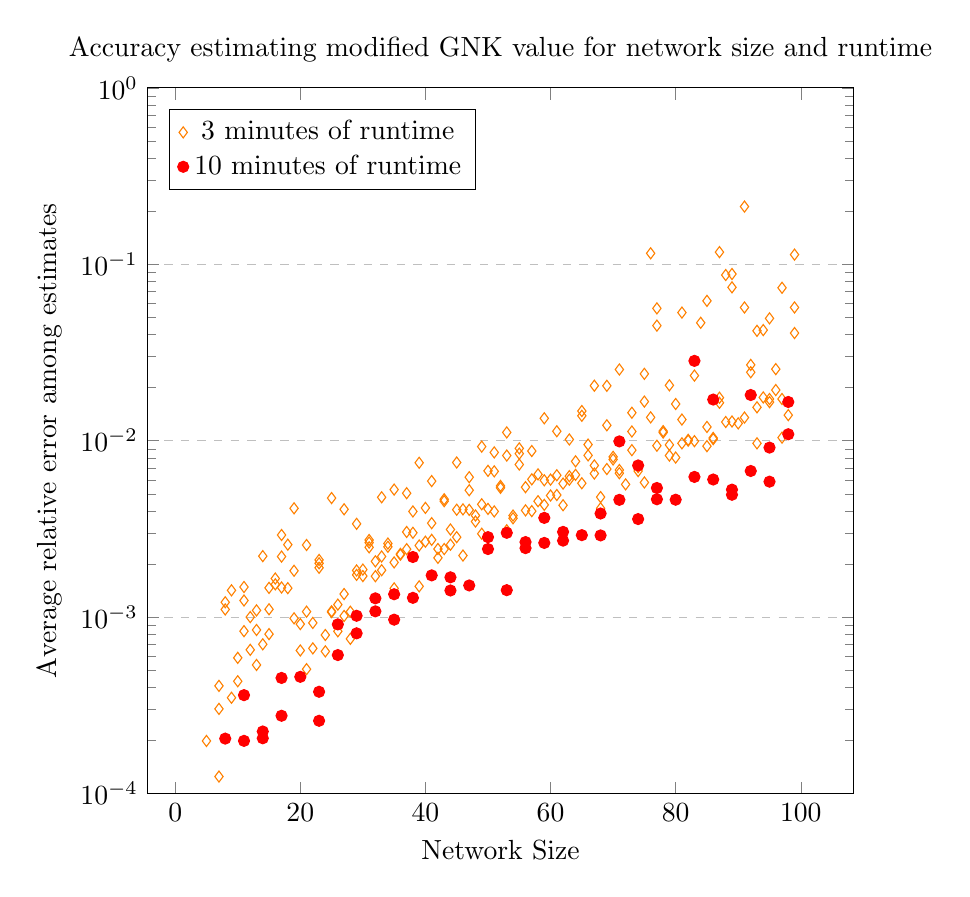
\begin{tikzpicture}
		\begin{axis}[
			title={Accuracy estimating modified GNK value for network size and runtime},
			xlabel={Network Size},
			ylabel={Average relative error among estimates},
			%xmin=0, xmax=0.25,
			ymin=0.0001, ymax=1.0,
			ymode=log,
			%xtick={0,0.05,0.1,0.15,0.2,0.25},
			%ytick={0,20,40,60,80,100},
			%yticklabel=$\pgfmathprintnumber{\tick}\%$,
			legend pos=north west,
			ymajorgrids=true,
			grid style=dashed,
			xticklabel style={/pgf/number format/fixed},
			width = 300,
			height = 300
		]
	%	\addplot [domain=5:15,dotted] {20+exp(exp(x/6.2))};
		\addplot[color=orange,only marks,mark=diamond] coordinates {
(7,0.000124846432046)
(9,0.000349362074085)
(11,0.00124222941518)
(13,0.00084580662349)
(15,0.000801583236527)
(17,0.00220431658342)
(19,0.00183164640034)
(21,0.0025649017953)
(23,0.00210995754038)
(25,0.00473061036627)
(27,0.00408531385556)
(29,0.00338104078055)
(31,0.00264677172477)
(33,0.0047801442004)
(35,0.00528516914309)
(37,0.00504239772522)
(39,0.00749977799528)
(41,0.00590305246372)
(43,0.00465727164346)
(45,0.00752693133478)
(47,0.00523965981561)
(49,0.00925944645823)
(51,0.00858391476366)
(53,0.0111435782515)
(55,0.00904646502096)
(57,0.00874408620603)
(59,0.0134009420369)
(61,0.0113124274953)
(63,0.0101657510766)
(65,0.0147341762157)
(67,0.0205141472091)
(69,0.0204764913685)
(71,0.0253312813336)
(73,0.0144118458985)
(75,0.02394286498)
(77,0.0449167019815)
(79,0.0206096637705)
(81,0.0532445997925)
(85,0.0620529404603)
(87,0.11719925893)
(89,0.074040615219)
(91,0.0569184449072)
(93,0.0419710612202)
(95,0.0493841921384)
(97,0.0736087900034)
(99,0.0569212660299)
(5,0.000198773008765)
(7,0.000407744729561)
(7,0.00030203334322)
(8,0.00121417461966)
(8,0.00110537817131)
(9,0.00141866481622)
(10,0.000587736031469)
(10,0.000433197835436)
(11,0.000833003424069)
(11,0.00148183780474)
(12,0.000652717485079)
(12,0.00100069147551)
(13,0.000535888589971)
(13,0.0010923780632)
(14,0.00221798060546)
(14,0.000701571822075)
(15,0.00146526302415)
(15,0.00110843825838)
(16,0.00153478099701)
(16,0.00165530968219)
(17,0.00147244059392)
(17,0.00292171158063)
(18,0.00257466150857)
(18,0.00146019035913)
(19,0.00413935310054)
(19,0.000984854650377)
(20,0.000913087823025)
(20,0.000647405471569)
(21,0.000506975456251)
(21,0.00107395672011)
(22,0.000927567910945)
(22,0.000665186002205)
(23,0.00201986852294)
(23,0.00190506406921)
(24,0.000639820142271)
(24,0.000792334026321)
(25,0.00107910701572)
(25,0.00106741530697)
(26,0.000831200889038)
(26,0.001178013224)
(27,0.00135186168514)
(27,0.00101545376012)
(28,0.00107335197392)
(28,0.000753723941028)
(29,0.00183920832934)
(29,0.00173603310834)
(30,0.00170985138939)
(30,0.00186055689586)
(31,0.00248752877425)
(31,0.00273821201003)
(32,0.00207141061644)
(32,0.00170630921974)
(33,0.00184563320948)
(33,0.00220666422401)
(34,0.00261345579349)
(34,0.00250566136421)
(35,0.00145532181738)
(35,0.00204272972711)
(36,0.00228404992204)
(36,0.00225933714185)
(37,0.00303894658767)
(37,0.0024283015975)
(38,0.00300795308548)
(38,0.00397239523048)
(39,0.0014948712232)
(39,0.00254757211551)
(40,0.00416220883856)
(40,0.00267674257379)
(41,0.00341086249742)
(41,0.00274167134022)
(42,0.00243460715137)
(42,0.00216802402016)
(43,0.0045429431476)
(43,0.00243201791179)
(44,0.00257436017038)
(44,0.0031394930501)
(45,0.00406347485638)
(45,0.00284040841552)
(46,0.00223361957965)
(46,0.00408187338654)
(47,0.00621155229259)
(47,0.00405687227955)
(48,0.00348237097269)
(48,0.0037691118267)
(49,0.00297039517578)
(49,0.00436222251494)
(50,0.006748950981)
(50,0.00410766447711)
(51,0.00670908443172)
(51,0.00397543990729)
(52,0.00554235567839)
(52,0.00540471876881)
(53,0.00824084761443)
(53,0.00310792483391)
(54,0.00363433436037)
(54,0.00376713945616)
(55,0.00844875182163)
(55,0.00732744960013)
(56,0.00402929471994)
(56,0.00545494825755)
(57,0.00399147611835)
(57,0.00604193725594)
(58,0.00454038668444)
(58,0.00644721921003)
(59,0.00596606446728)
(59,0.00432958920691)
(60,0.00601779650865)
(60,0.00489093054392)
(61,0.00492231997481)
(61,0.00637153496756)
(62,0.00430846933583)
(62,0.00571567178718)
(63,0.0060166079485)
(63,0.00629811025019)
(64,0.00640649255773)
(64,0.00763967913687)
(65,0.00573940477132)
(65,0.0138494680438)
(66,0.00950896711587)
(66,0.00826076933508)
(67,0.00651406615877)
(67,0.00724154201149)
(68,0.00479242033538)
(68,0.00414009158155)
(69,0.00691061325658)
(69,0.0122340696862)
(70,0.0081037292405)
(70,0.0078300002664)
(71,0.00654540779197)
(71,0.00682384509876)
(72,0.00565662022543)
(73,0.00884093704595)
(73,0.0112777832194)
(74,0.00708325114328)
(74,0.0067307025997)
(75,0.00580076774973)
(75,0.0166710544997)
(76,0.0135653233246)
(76,0.115409477308)
(77,0.0562417271889)
(77,0.00936786247095)
(78,0.0111215791274)
(78,0.0113334495573)
(79,0.00823906874579)
(79,0.00947459165119)
(80,0.0161486868496)
(80,0.00802704625735)
(81,0.00966195470957)
(81,0.0131841104013)
(82,0.0101128126268)
(82,0.0100115250202)
(83,0.00994581004764)
(83,0.0234048108537)
(84,0.0466033245366)
(85,0.00931630151593)
(85,0.0119695395793)
(86,0.0102139379601)
(86,0.0103722797318)
(87,0.0175397536068)
(87,0.0164074281767)
(88,0.0869332312724)
(88,0.0127678076343)
(89,0.0881032048071)
(89,0.0128528308022)
(90,0.0125394314882)
(91,0.21235279003)
(91,0.0135224949691)
(92,0.0269092164032)
(92,0.0244399626971)
(93,0.0154693117288)
(93,0.00966429818161)
(94,0.0423744311321)
(94,0.0176065608411)
(95,0.017242036729)
(95,0.0165513968124)
(96,0.0193783901172)
(96,0.0254570264808)
(97,0.0172404117218)
(97,0.0104124125146)
(98,0.0139618278174)
(99,0.0407574094971)
(99,0.113474875413)
			}node[pos=0.8](endofplotsquare){} ;
\addplot[color=red,only marks,mark=*] coordinates {
(8,0.000204879456534)
(11,0.000198954708294)
(14,0.000224818148859)
(17,0.000452273026779)
(23,0.000377511363366)
(26,0.000909889613207)
(29,0.000809735581049)
(32,0.00107871411898)
(35,0.00134833546078)
(38,0.00128650914677)
(44,0.00141620500018)
(50,0.00243255599249)
(53,0.00300619010686)
(56,0.00266403262447)
(59,0.00365306085279)
(62,0.00271466495323)
(68,0.00386736101309)
(71,0.00462278912607)
(74,0.0035967562431)
(77,0.00465761537595)
(80,0.00462987381052)
(83,0.00623532230411)
(86,0.0171156268226)
(89,0.00528077744006)
(92,0.00673753567814)
(95,0.00913995479916)
(98,0.0165834905391)
(5,0.0000773935779233)
(8,0.0000733345523358)
(11,0.000361375533438)
(14,0.000205841984163)
(17,0.000276048066766)
(20,0.000458867046201)
(23,0.000258513233782)
(26,0.000609668878525)
(29,0.00101805824417)
(32,0.0012780948209)
(35,0.000967653390575)
(38,0.00219240621832)
(41,0.00172504220769)
(44,0.00168192681336)
(47,0.00151247011605)
(50,0.00284133781795)
(53,0.00142210304518)
(56,0.00246181621126)
(59,0.00263488361456)
(62,0.00304277252977)
(65,0.00291604974117)
(68,0.00290600963346)
(71,0.00991308235081)
(74,0.00724174012946)
(77,0.00539653837363)
(83,0.0283508439613)
(86,0.00602785697971)
(89,0.00494013614493)
(92,0.0181610789112)
(95,0.00586061614028)
(98,0.010881684427)
			}node[pos=0.8](endofplotsquare){} ;
			
\addlegendentry{3 minutes of runtime}
\addlegendentry{10 minutes of runtime}
		\end{axis}
		\end{tikzpicture}
		%\vspace{-18pt}
		\caption{Average magnitude of error relative to the magnitude of the estimated modified GNK value between 8 independent simultaneous estimations on randomly generated networks of different sizes, for 3 and 10 minutes runtime on a desktop computer.}
		\label{fig:performance_graph4}
    \end{figure}




\fi

\iffigures

    \begin{figure}[]
        \centering
		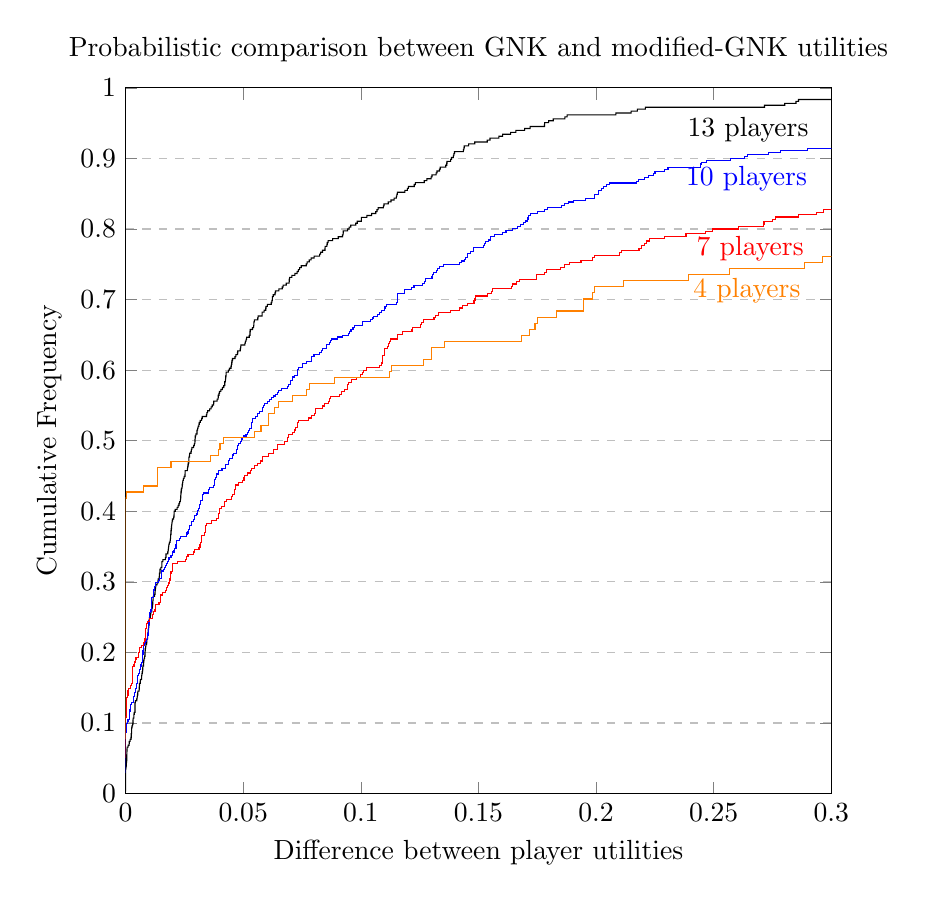
\begin{tikzpicture}
		\begin{axis}[
			title={Probabilistic comparison between GNK and modified-GNK utilities},
			xlabel={Difference between player utilities},
			ylabel={Cumulative Frequency},
			xmin=0.0, xmax=0.3,
			ymin=0.0, ymax=1.0,
			%xmode=log,
			%xtick={0,0.05,0.1,0.15,0.2,0.25},
			%ytick={0,20,40,60,80,100},
			%yticklabel=$\pgfmathprintnumber{\tick}\%$,
			legend pos=south west,
			ymajorgrids=true,
			grid style=dashed,
			xticklabel style={/pgf/number format/fixed},
			width = 300,
			height = 300
		]
	%	\addplot [domain=5:15,dotted] {20+exp(exp(x/6.2))};
		\addplot[color=black] coordinates {
%(0.530799741778,1.0)(0.530799741778,0.997260273973)(0.491707332267,0.997260273973)(0.491707332267,0.994520547945)(0.425412132355,0.994520547945)(0.425412132355,0.991780821918)(0.357182697513,0.991780821918)(0.357182697513,0.98904109589)(0.319610241692,0.98904109589)(0.319610241692,0.986301369863)
(0.309037212975,0.986301369863)(0.309037212975,0.983561643836)(0.286057431393,0.983561643836)(0.286057431393,0.980821917808)(0.284994898465,0.980821917808)(0.284994898465,0.978082191781)(0.280206419368,0.978082191781)(0.280206419368,0.975342465753)(0.27159325427,0.975342465753)(0.27159325427,0.972602739726)(0.220954455678,0.972602739726)(0.220954455678,0.969863013699)(0.217521096865,0.969863013699)(0.217521096865,0.967123287671)(0.214905030785,0.967123287671)(0.214905030785,0.964383561644)(0.208402409616,0.964383561644)(0.208402409616,0.961643835616)(0.187697416466,0.961643835616)(0.187697416466,0.958904109589)(0.186718359139,0.958904109589)(0.186718359139,0.956164383562)(0.18178731688,0.956164383562)(0.18178731688,0.953424657534)(0.179827432506,0.953424657534)(0.179827432506,0.950684931507)(0.178096915502,0.950684931507)(0.178096915502,0.947945205479)(0.178050564331,0.947945205479)(0.178050564331,0.945205479452)(0.171944702883,0.945205479452)(0.171944702883,0.942465753425)(0.169625246021,0.942465753425)(0.169625246021,0.939726027397)(0.16591677708,0.939726027397)(0.16591677708,0.93698630137)(0.163674232334,0.93698630137)(0.163674232334,0.934246575342)(0.160237221381,0.934246575342)(0.160237221381,0.931506849315)(0.158698006367,0.931506849315)(0.158698006367,0.928767123288)(0.154907706605,0.928767123288)(0.154907706605,0.92602739726)(0.15373666429,0.92602739726)(0.15373666429,0.923287671233)(0.148430597482,0.923287671233)(0.148430597482,0.920547945205)(0.145835465344,0.920547945205)(0.145835465344,0.917808219178)(0.143930102797,0.917808219178)(0.143930102797,0.915068493151)(0.143779203067,0.915068493151)(0.143779203067,0.912328767123)(0.143585669431,0.912328767123)(0.143585669431,0.909589041096)(0.139785084882,0.909589041096)(0.139785084882,0.906849315068)(0.139530522155,0.906849315068)(0.139530522155,0.904109589041)(0.139324332123,0.904109589041)(0.139324332123,0.901369863014)(0.138515330876,0.901369863014)(0.138515330876,0.898630136986)(0.138186833213,0.898630136986)(0.138186833213,0.895890410959)(0.136604638094,0.895890410959)(0.136604638094,0.893150684932)(0.136511145943,0.893150684932)(0.136511145943,0.890410958904)(0.136107505064,0.890410958904)(0.136107505064,0.887671232877)(0.133735989613,0.887671232877)(0.133735989613,0.884931506849)(0.133446463765,0.884931506849)(0.133446463765,0.882191780822)(0.132387093034,0.882191780822)(0.132387093034,0.879452054795)(0.132022599944,0.879452054795)(0.132022599944,0.876712328767)(0.130262477849,0.876712328767)(0.130262477849,0.87397260274)(0.129872196041,0.87397260274)(0.129872196041,0.871232876712)(0.128081983861,0.871232876712)(0.128081983861,0.868493150685)(0.126962731778,0.868493150685)(0.126962731778,0.865753424658)(0.123143151789,0.865753424658)(0.123143151789,0.86301369863)(0.12267651949,0.86301369863)(0.12267651949,0.860273972603)(0.120204691629,0.860273972603)(0.120204691629,0.857534246575)(0.119785096614,0.857534246575)(0.119785096614,0.854794520548)(0.118714496392,0.854794520548)(0.118714496392,0.852054794521)(0.115539121674,0.852054794521)(0.115539121674,0.849315068493)(0.115337593827,0.849315068493)(0.115337593827,0.846575342466)(0.115074604798,0.846575342466)(0.115074604798,0.843835616438)(0.114117148634,0.843835616438)(0.114117148634,0.841095890411)(0.112815831781,0.841095890411)(0.112815831781,0.838356164384)(0.11164497987,0.838356164384)(0.11164497987,0.835616438356)(0.109817718445,0.835616438356)(0.109817718445,0.832876712329)(0.109541818422,0.832876712329)(0.109541818422,0.830136986301)(0.107312322151,0.830136986301)(0.107312322151,0.827397260274)(0.106869456164,0.827397260274)(0.106869456164,0.824657534247)(0.106317931934,0.824657534247)(0.106317931934,0.821917808219)(0.10455238503,0.821917808219)(0.10455238503,0.819178082192)(0.102535786498,0.819178082192)(0.102535786498,0.816438356164)(0.10023872574,0.816438356164)(0.10023872574,0.813698630137)(0.100228252616,0.813698630137)(0.100228252616,0.81095890411)(0.0984526654456,0.81095890411)(0.0984526654456,0.808219178082)(0.0978265984652,0.808219178082)(0.0978265984652,0.805479452055)(0.0956973295849,0.805479452055)(0.0956973295849,0.802739726027)(0.0949821224902,0.802739726027)(0.0949821224902,0.8)(0.0943939343696,0.8)(0.0943939343696,0.797260273973)(0.0925081476802,0.797260273973)(0.0925081476802,0.794520547945)(0.0924878678404,0.794520547945)(0.0924878678404,0.791780821918)(0.0922063886543,0.791780821918)(0.0922063886543,0.78904109589)(0.0903893562138,0.78904109589)(0.0903893562138,0.786301369863)(0.0879995155483,0.786301369863)(0.0879995155483,0.783561643836)(0.0860958223587,0.783561643836)(0.0860958223587,0.780821917808)(0.0857040669837,0.780821917808)(0.0857040669837,0.778082191781)(0.0855735236653,0.778082191781)(0.0855735236653,0.775342465753)(0.0848036534751,0.775342465753)(0.0848036534751,0.772602739726)(0.0847456778207,0.772602739726)(0.0847456778207,0.769863013699)(0.0837087994827,0.769863013699)(0.0837087994827,0.767123287671)(0.0829140509123,0.767123287671)(0.0829140509123,0.764383561644)(0.0824979742273,0.764383561644)(0.0824979742273,0.761643835616)(0.0801267224376,0.761643835616)(0.0801267224376,0.758904109589)(0.0788508338915,0.758904109589)(0.0788508338915,0.756164383562)(0.078066826337,0.756164383562)(0.078066826337,0.753424657534)(0.0771322806037,0.753424657534)(0.0771322806037,0.750684931507)(0.07680086899,0.750684931507)(0.07680086899,0.747945205479)(0.074658919858,0.747945205479)(0.074658919858,0.745205479452)(0.0739416287963,0.745205479452)(0.0739416287963,0.742465753425)(0.0734545139772,0.742465753425)(0.0734545139772,0.739726027397)(0.0729256732617,0.739726027397)(0.0729256732617,0.73698630137)(0.0719461866967,0.73698630137)(0.0719461866967,0.734246575342)(0.0706676719056,0.734246575342)(0.0706676719056,0.731506849315)(0.0696974915765,0.731506849315)(0.0696974915765,0.728767123288)(0.0695507929349,0.728767123288)(0.0695507929349,0.72602739726)(0.0695252195489,0.72602739726)(0.0695252195489,0.723287671233)(0.0682753558075,0.723287671233)(0.0682753558075,0.720547945205)(0.0669800326308,0.720547945205)(0.0669800326308,0.717808219178)(0.06660160903,0.717808219178)(0.06660160903,0.715068493151)(0.0651212614169,0.715068493151)(0.0651212614169,0.712328767123)(0.0637010737122,0.712328767123)(0.0637010737122,0.709589041096)(0.0635064928705,0.709589041096)(0.0635064928705,0.706849315068)(0.0627312623723,0.706849315068)(0.0627312623723,0.704109589041)(0.0623727218433,0.704109589041)(0.0623727218433,0.701369863014)(0.0623672111018,0.701369863014)(0.0623672111018,0.698630136986)(0.0621971071668,0.698630136986)(0.0621971071668,0.695890410959)(0.0618938447442,0.695890410959)(0.0618938447442,0.693150684932)(0.0602443841631,0.693150684932)(0.0602443841631,0.690410958904)(0.0596664040295,0.690410958904)(0.0596664040295,0.687671232877)(0.0595548389228,0.687671232877)(0.0595548389228,0.684931506849)(0.0588604764123,0.684931506849)(0.0588604764123,0.682191780822)(0.058019158752,0.682191780822)(0.058019158752,0.679452054795)(0.058019158752,0.679452054795)(0.058019158752,0.676712328767)(0.0563170235772,0.676712328767)(0.0563170235772,0.67397260274)(0.0561500372567,0.67397260274)(0.0561500372567,0.671232876712)(0.0547106292878,0.671232876712)(0.0547106292878,0.668493150685)(0.0545352626028,0.668493150685)(0.0545352626028,0.665753424658)(0.0545168172155,0.665753424658)(0.0545168172155,0.66301369863)(0.0544180134667,0.66301369863)(0.0544180134667,0.660273972603)(0.053929255253,0.660273972603)(0.053929255253,0.657534246575)(0.0529557324488,0.657534246575)(0.0529557324488,0.654794520548)(0.0528871542549,0.654794520548)(0.0528871542549,0.652054794521)(0.0528614560227,0.652054794521)(0.0528614560227,0.649315068493)(0.0525525925911,0.649315068493)(0.0525525925911,0.646575342466)(0.0514435034638,0.646575342466)(0.0514435034638,0.643835616438)(0.0512175470147,0.643835616438)(0.0512175470147,0.641095890411)(0.0509279553047,0.641095890411)(0.0509279553047,0.638356164384)(0.0507111346228,0.638356164384)(0.0507111346228,0.635616438356)(0.0490102868845,0.635616438356)(0.0490102868845,0.632876712329)(0.0488673970345,0.632876712329)(0.0488673970345,0.630136986301)(0.0487178165363,0.630136986301)(0.0487178165363,0.627397260274)(0.0476693856799,0.627397260274)(0.0476693856799,0.624657534247)(0.0475444019072,0.624657534247)(0.0475444019072,0.621917808219)(0.0468628880003,0.621917808219)(0.0468628880003,0.619178082192)(0.046483090322,0.619178082192)(0.046483090322,0.616438356164)(0.0454352067453,0.616438356164)(0.0454352067453,0.613698630137)(0.045227902016,0.613698630137)(0.045227902016,0.61095890411)(0.0451180839459,0.61095890411)(0.0451180839459,0.608219178082)(0.0449659605317,0.608219178082)(0.0449659605317,0.605479452055)(0.0447802274642,0.605479452055)(0.0447802274642,0.602739726027)(0.0441667740341,0.602739726027)(0.0441667740341,0.6)(0.0436637002789,0.6)(0.0436637002789,0.597260273973)(0.0427321018961,0.597260273973)(0.0427321018961,0.594520547945)(0.0426908388164,0.594520547945)(0.0426908388164,0.591780821918)(0.0425635929965,0.591780821918)(0.0425635929965,0.58904109589)(0.0425223005892,0.58904109589)(0.0425223005892,0.586301369863)(0.0423739055348,0.586301369863)(0.0423739055348,0.583561643836)(0.0421334558118,0.583561643836)(0.0421334558118,0.580821917808)(0.0421244079829,0.580821917808)(0.0421244079829,0.578082191781)(0.041726259792,0.578082191781)(0.041726259792,0.575342465753)(0.0411373662782,0.575342465753)(0.0411373662782,0.572602739726)(0.0404624577605,0.572602739726)(0.0404624577605,0.569863013699)(0.0398877455756,0.569863013699)(0.0398877455756,0.567123287671)(0.0396842374671,0.567123287671)(0.0396842374671,0.564383561644)(0.0393797775845,0.564383561644)(0.0393797775845,0.561643835616)(0.0392968795591,0.561643835616)(0.0392968795591,0.558904109589)(0.0388920102273,0.558904109589)(0.0388920102273,0.556164383562)(0.037475936879,0.556164383562)(0.037475936879,0.553424657534)(0.0373986033279,0.553424657534)(0.0373986033279,0.550684931507)(0.0368389222752,0.550684931507)(0.0368389222752,0.547945205479)(0.0363588003786,0.547945205479)(0.0363588003786,0.545205479452)(0.0356779179593,0.545205479452)(0.0356779179593,0.542465753425)(0.0348720617843,0.542465753425)(0.0348720617843,0.539726027397)(0.0345064534148,0.539726027397)(0.0345064534148,0.53698630137)(0.034359263457,0.53698630137)(0.034359263457,0.534246575342)(0.0325507379994,0.534246575342)(0.0325507379994,0.531506849315)(0.0322844931228,0.531506849315)(0.0322844931228,0.528767123288)(0.0316991973193,0.528767123288)(0.0316991973193,0.52602739726)(0.031288184579,0.52602739726)(0.031288184579,0.523287671233)(0.0311552922598,0.523287671233)(0.0311552922598,0.520547945205)(0.030826317004,0.520547945205)(0.030826317004,0.517808219178)(0.0306161782635,0.517808219178)(0.0306161782635,0.515068493151)(0.0303266151927,0.515068493151)(0.0303266151927,0.512328767123)(0.0303207047721,0.512328767123)(0.0303207047721,0.509589041096)(0.0298579937364,0.509589041096)(0.0298579937364,0.506849315068)(0.0295931317552,0.506849315068)(0.0295931317552,0.504109589041)(0.0295569218748,0.504109589041)(0.0295569218748,0.501369863014)(0.0294966596898,0.501369863014)(0.0294966596898,0.498630136986)(0.0294394182159,0.498630136986)(0.0294394182159,0.495890410959)(0.0292314445595,0.495890410959)(0.0292314445595,0.493150684932)(0.0288820269963,0.493150684932)(0.0288820269963,0.490410958904)(0.0281378859445,0.490410958904)(0.0281378859445,0.487671232877)(0.0279714016933,0.487671232877)(0.0279714016933,0.484931506849)(0.0277785062448,0.484931506849)(0.0277785062448,0.482191780822)(0.0272041228618,0.482191780822)(0.0272041228618,0.479452054795)(0.0271326532963,0.479452054795)(0.0271326532963,0.476712328767)(0.0268815063204,0.476712328767)(0.0268815063204,0.47397260274)(0.0268807428699,0.47397260274)(0.0268807428699,0.471232876712)(0.0268663024777,0.471232876712)(0.0268663024777,0.468493150685)(0.0266406224441,0.468493150685)(0.0266406224441,0.465753424658)(0.0264916252168,0.465753424658)(0.0264916252168,0.46301369863)(0.0263391896179,0.46301369863)(0.0263391896179,0.460273972603)(0.0262276262171,0.460273972603)(0.0262276262171,0.457534246575)(0.0253201057798,0.457534246575)(0.0253201057798,0.454794520548)(0.0252600947714,0.454794520548)(0.0252600947714,0.452054794521)(0.0252419475712,0.452054794521)(0.0252419475712,0.449315068493)(0.0248395237233,0.449315068493)(0.0248395237233,0.446575342466)(0.0245238522598,0.446575342466)(0.0245238522598,0.443835616438)(0.0243501994916,0.443835616438)(0.0243501994916,0.441095890411)(0.0242162153446,0.441095890411)(0.0242162153446,0.438356164384)(0.0240706181789,0.438356164384)(0.0240706181789,0.435616438356)(0.023991424534,0.435616438356)(0.023991424534,0.432876712329)(0.0237289833425,0.432876712329)(0.0237289833425,0.430136986301)(0.0236291227621,0.430136986301)(0.0236291227621,0.427397260274)(0.0235390795095,0.427397260274)(0.0235390795095,0.424657534247)(0.023479286896,0.424657534247)(0.023479286896,0.421917808219)(0.0234322200843,0.421917808219)(0.0234322200843,0.419178082192)(0.0233839510275,0.419178082192)(0.0233839510275,0.416438356164)(0.0232450069899,0.416438356164)(0.0232450069899,0.413698630137)(0.0229702523376,0.413698630137)(0.0229702523376,0.41095890411)(0.0226757930079,0.41095890411)(0.0226757930079,0.408219178082)(0.0223064734331,0.408219178082)(0.0223064734331,0.405479452055)(0.0219106837603,0.405479452055)(0.0219106837603,0.402739726027)(0.0210852715654,0.402739726027)(0.0210852715654,0.4)(0.0205953737963,0.4)(0.0205953737963,0.397260273973)(0.0205840001233,0.397260273973)(0.0205840001233,0.394520547945)(0.0205669149342,0.394520547945)(0.0205669149342,0.391780821918)(0.0203733513268,0.391780821918)(0.0203733513268,0.38904109589)(0.019901843789,0.38904109589)(0.019901843789,0.386301369863)(0.0197527943102,0.386301369863)(0.0197527943102,0.383561643836)(0.0196801633948,0.383561643836)(0.0196801633948,0.380821917808)(0.0195765807412,0.380821917808)(0.0195765807412,0.378082191781)(0.0194918867551,0.378082191781)(0.0194918867551,0.375342465753)(0.0193916503192,0.375342465753)(0.0193916503192,0.372602739726)(0.0192804985562,0.372602739726)(0.0192804985562,0.369863013699)(0.0192701876001,0.369863013699)(0.0192701876001,0.367123287671)(0.0191382319738,0.367123287671)(0.0191382319738,0.364383561644)(0.0190960091769,0.364383561644)(0.0190960091769,0.361643835616)(0.0189898803636,0.361643835616)(0.0189898803636,0.358904109589)(0.0189163007626,0.358904109589)(0.0189163007626,0.356164383562)(0.0185637862952,0.356164383562)(0.0185637862952,0.353424657534)(0.0183529690548,0.353424657534)(0.0183529690548,0.350684931507)(0.0182847181055,0.350684931507)(0.0182847181055,0.347945205479)(0.0181553079211,0.347945205479)(0.0181553079211,0.345205479452)(0.0180427569802,0.345205479452)(0.0180427569802,0.342465753425)(0.0178958091802,0.342465753425)(0.0178958091802,0.339726027397)(0.0171599095053,0.339726027397)(0.0171599095053,0.33698630137)(0.0171510965367,0.33698630137)(0.0171510965367,0.334246575342)(0.016882750954,0.334246575342)(0.016882750954,0.331506849315)(0.0158249613515,0.331506849315)(0.0158249613515,0.328767123288)(0.0154073009714,0.328767123288)(0.0154073009714,0.32602739726)(0.0153988166286,0.32602739726)(0.0153988166286,0.323287671233)(0.0153874302947,0.323287671233)(0.0153874302947,0.320547945205)(0.0149849730024,0.320547945205)(0.0149849730024,0.317808219178)(0.014621992753,0.317808219178)(0.014621992753,0.315068493151)(0.0145985958486,0.315068493151)(0.0145985958486,0.312328767123)(0.0143306091424,0.312328767123)(0.0143306091424,0.309589041096)(0.0143219468319,0.309589041096)(0.0143219468319,0.306849315068)(0.0142356117949,0.306849315068)(0.0142356117949,0.304109589041)(0.0138006496195,0.304109589041)(0.0138006496195,0.301369863014)(0.0137665589999,0.301369863014)(0.0137665589999,0.298630136986)(0.0134003240583,0.298630136986)(0.0134003240583,0.295890410959)(0.0128604760338,0.295890410959)(0.0128604760338,0.293150684932)(0.0126948234609,0.293150684932)(0.0126948234609,0.290410958904)(0.0126612105684,0.290410958904)(0.0126612105684,0.287671232877)(0.012558235327,0.287671232877)(0.012558235327,0.284931506849)(0.0124957532224,0.284931506849)(0.0124957532224,0.282191780822)(0.012284900863,0.282191780822)(0.012284900863,0.279452054795)(0.0117082313606,0.279452054795)(0.0117082313606,0.276712328767)(0.0116735074537,0.276712328767)(0.0116735074537,0.27397260274)(0.0116078488996,0.27397260274)(0.0116078488996,0.271232876712)(0.0115104227347,0.271232876712)(0.0115104227347,0.268493150685)(0.0114054315825,0.268493150685)(0.0114054315825,0.265753424658)(0.0113049276365,0.265753424658)(0.0113049276365,0.26301369863)(0.0111767324766,0.26301369863)(0.0111767324766,0.260273972603)(0.0111214176319,0.260273972603)(0.0111214176319,0.257534246575)(0.0107425694064,0.257534246575)(0.0107425694064,0.254794520548)(0.0105748697077,0.254794520548)(0.0105748697077,0.252054794521)(0.0105041178321,0.252054794521)(0.0105041178321,0.249315068493)(0.0101048812783,0.249315068493)(0.0101048812783,0.246575342466)(0.0100537537352,0.246575342466)(0.0100537537352,0.243835616438)(0.0100426336695,0.243835616438)(0.0100426336695,0.241095890411)(0.0100082975313,0.241095890411)(0.0100082975313,0.238356164384)(0.0098415404511,0.238356164384)(0.0098415404511,0.235616438356)(0.00978439582691,0.235616438356)(0.00978439582691,0.232876712329)(0.00959799727247,0.232876712329)(0.00959799727247,0.230136986301)(0.00955461506239,0.230136986301)(0.00955461506239,0.227397260274)(0.00934079801624,0.227397260274)(0.00934079801624,0.224657534247)(0.0093243712393,0.224657534247)(0.0093243712393,0.221917808219)(0.00932081415261,0.221917808219)(0.00932081415261,0.219178082192)(0.00903579175035,0.219178082192)(0.00903579175035,0.216438356164)(0.0089916958488,0.216438356164)(0.0089916958488,0.213698630137)(0.00885808923729,0.213698630137)(0.00885808923729,0.21095890411)(0.0086249960169,0.21095890411)(0.0086249960169,0.208219178082)(0.00847068487875,0.208219178082)(0.00847068487875,0.205479452055)(0.0083485958486,0.205479452055)(0.0083485958486,0.202739726027)(0.00830708977519,0.202739726027)(0.00830708977519,0.2)(0.00824996310299,0.2)(0.00824996310299,0.197260273973)(0.00822298803597,0.197260273973)(0.00822298803597,0.194520547945)(0.00806469611627,0.194520547945)(0.00806469611627,0.191780821918)(0.00784326081057,0.191780821918)(0.00784326081057,0.18904109589)(0.00768459519191,0.18904109589)(0.00768459519191,0.186301369863)(0.00759564030064,0.186301369863)(0.00759564030064,0.183561643836)(0.00759474537174,0.183561643836)(0.00759474537174,0.180821917808)(0.0073194035507,0.180821917808)(0.0073194035507,0.178082191781)(0.00726776156327,0.178082191781)(0.00726776156327,0.175342465753)(0.00722255111882,0.175342465753)(0.00722255111882,0.172602739726)(0.00704511150422,0.172602739726)(0.00704511150422,0.169863013699)(0.00690753284637,0.169863013699)(0.00690753284637,0.167123287671)(0.00679330094975,0.167123287671)(0.00679330094975,0.164383561644)(0.00679330094975,0.164383561644)(0.00679330094975,0.161643835616)(0.00629016066525,0.161643835616)(0.00629016066525,0.158904109589)(0.00620076229701,0.158904109589)(0.00620076229701,0.156164383562)(0.00591624205767,0.156164383562)(0.00591624205767,0.153424657534)(0.00583823846884,0.153424657534)(0.00583823846884,0.150684931507)(0.00580993740412,0.150684931507)(0.00580993740412,0.147945205479)(0.00573006046105,0.147945205479)(0.00573006046105,0.145205479452)(0.0051954786379,0.145205479452)(0.0051954786379,0.142465753425)(0.0051428523288,0.142465753425)(0.0051428523288,0.139726027397)(0.00500624606826,0.139726027397)(0.00500624606826,0.13698630137)(0.00487811579137,0.13698630137)(0.00487811579137,0.134246575342)(0.00473520565905,0.134246575342)(0.00473520565905,0.131506849315)(0.00413487843447,0.131506849315)(0.00413487843447,0.128767123288)(0.00397102897103,0.128767123288)(0.00397102897103,0.12602739726)(0.00397102897103,0.12602739726)(0.00397102897103,0.123287671233)(0.00397102897103,0.123287671233)(0.00397102897103,0.120547945205)(0.00397102897103,0.120547945205)(0.00397102897103,0.117808219178)(0.00397102897103,0.117808219178)(0.00397102897103,0.115068493151)(0.0036764862994,0.115068493151)(0.0036764862994,0.112328767123)(0.00347667577682,0.112328767123)(0.00347667577682,0.109589041096)(0.00347519625076,0.109589041096)(0.00347519625076,0.106849315068)(0.00317334415099,0.106849315068)(0.00317334415099,0.104109589041)(0.00312249279547,0.104109589041)(0.00312249279547,0.101369863014)(0.00311747237996,0.101369863014)(0.00311747237996,0.0986301369863)(0.00298729819113,0.0986301369863)(0.00298729819113,0.0958904109589)(0.00271323278181,0.0958904109589)(0.00271323278181,0.0931506849315)(0.00252438729159,0.0931506849315)(0.00252438729159,0.0904109589041)(0.00252072917122,0.0904109589041)(0.00252072917122,0.0876712328767)(0.00252072917122,0.0876712328767)(0.00252072917122,0.0849315068493)(0.00240459913893,0.0849315068493)(0.00240459913893,0.0821917808219)(0.002401933569,0.0821917808219)(0.002401933569,0.0794520547945)(0.00225926020951,0.0794520547945)(0.00225926020951,0.0767123287671)(0.00188298412488,0.0767123287671)(0.00188298412488,0.0739726027397)(0.00155354182162,0.0739726027397)(0.00155354182162,0.0712328767123)(0.00147947127062,0.0712328767123)(0.00147947127062,0.0684931506849)(0.00107683430451,0.0684931506849)(0.00107683430451,0.0657534246575)(0.000604316117921,0.0657534246575)(0.000604316117921,0.0630136986301)(0.000598013098013,0.0630136986301)(0.000598013098013,0.0602739726027)(0.000523608336108,0.0602739726027)(0.000523608336108,0.0575342465753)(0.000507073944574,0.0575342465753)(0.000507073944574,0.0547945205479)(0.0004954998705,0.0547945205479)(0.0004954998705,0.0520547945205)(0.000487082362082,0.0520547945205)(0.000487082362082,0.0493150684932)(0.000480769230769,0.0493150684932)(0.000480769230769,0.0465753424658)(0.000405609791084,0.0465753424658)(0.000405609791084,0.0438356164384)(0.000245933334418,0.0438356164384)(0.000245933334418,0.041095890411)(0.000243017908125,0.041095890411)(0.000243017908125,0.0383561643836)(0.0,0.0328767123288)(0.0,0.0301369863014)(0.0,0.0301369863014)(0.0,0.027397260274)(0.0,0.027397260274)(0.0,0.0246575342466)(0.0,0.0246575342466)(0.0,0.0219178082192)(0.0,0.0219178082192)(0.0,0.0191780821918)(0.0,0.0191780821918)(0.0,0.0164383561644)(0.0,0.0164383561644)(0.0,0.013698630137)(0.0,0.013698630137)(0.0,0.0109589041096)(0.0,0.0109589041096)(0.0,0.00821917808219)(0.0,0.00821917808219)(0.0,0.00547945205479)(0.0,0.00547945205479)(0.0,0.0027397260274)
			}node[pos=0.045](endofplotsquare){} ;
		\node [below,color=black] at (endofplotsquare) {13 players};
		\addplot[color=blue] coordinates {
%(2.89289156139,0.973045822102)(2.89289156139,0.970350404313)(1.6628340622,0.970350404313)(1.6628340622,0.967654986523)(1.65134434726,0.967654986523)(1.65134434726,0.964959568733)(1.60972627146,0.964959568733)(1.60972627146,0.962264150943)(1.5310100826,0.962264150943)(1.5310100826,0.959568733154)(1.51082968902,0.959568733154)(1.51082968902,0.956873315364)(0.990353701004,0.956873315364)(0.990353701004,0.954177897574)(0.73522418558,0.954177897574)(0.73522418558,0.951482479784)(0.721540773681,0.951482479784)(0.721540773681,0.948787061995)(0.719765249636,0.948787061995)(0.719765249636,0.946091644205)(0.714749722992,0.946091644205)(0.714749722992,0.943396226415)(0.535346641639,0.943396226415)(0.535346641639,0.940700808625)(0.502562535431,0.940700808625)(0.502562535431,0.938005390836)(0.478946208113,0.938005390836)(0.478946208113,0.935309973046)(0.478809291729,0.935309973046)(0.478809291729,0.932614555256)(0.43271699298,0.932614555256)(0.43271699298,0.929919137466)(0.407265979308,0.929919137466)(0.407265979308,0.927223719677)(0.375452980401,0.927223719677)(0.375452980401,0.924528301887)(0.365920086753,0.924528301887)(0.365920086753,0.921832884097)(0.352431677114,0.921832884097)(0.352431677114,0.919137466307)(0.344982993197,0.919137466307)(0.344982993197,0.916442048518)(0.325752475655,0.916442048518)
(0.325752475655,0.913746630728)(0.289891603868,0.913746630728)(0.289891603868,0.911051212938)(0.278348074664,0.911051212938)(0.278348074664,0.908355795148)(0.27340316507,0.908355795148)(0.27340316507,0.905660377358)(0.264502728175,0.905660377358)(0.264502728175,0.902964959569)(0.263151709613,0.902964959569)(0.263151709613,0.900269541779)(0.257024421553,0.900269541779)(0.257024421553,0.897574123989)(0.247116900082,0.897574123989)(0.247116900082,0.894878706199)(0.244734684598,0.894878706199)(0.244734684598,0.89218328841)(0.244431489757,0.89218328841)(0.244431489757,0.88948787062)(0.244355686921,0.88948787062)(0.244355686921,0.88679245283)(0.230562816398,0.88679245283)(0.230562816398,0.88409703504)(0.229232427867,0.88409703504)(0.229232427867,0.881401617251)(0.225056604223,0.881401617251)(0.225056604223,0.878706199461)(0.224482664984,0.878706199461)(0.224482664984,0.876010781671)(0.222227560124,0.876010781671)(0.222227560124,0.873315363881)(0.220562864143,0.873315363881)(0.220562864143,0.870619946092)(0.217962684982,0.870619946092)(0.217962684982,0.867924528302)(0.217338171505,0.867924528302)(0.217338171505,0.865229110512)(0.205672357955,0.865229110512)(0.205672357955,0.862533692722)(0.204575994355,0.862533692722)(0.204575994355,0.859838274933)(0.202958644266,0.859838274933)(0.202958644266,0.857142857143)(0.202215162203,0.857142857143)(0.202215162203,0.854447439353)(0.201146002605,0.854447439353)(0.201146002605,0.851752021563)(0.200904078236,0.851752021563)(0.200904078236,0.849056603774)(0.199479753745,0.849056603774)(0.199479753745,0.846361185984)(0.199181547619,0.846361185984)(0.199181547619,0.843665768194)(0.195622053349,0.843665768194)(0.195622053349,0.840970350404)(0.190234452104,0.840970350404)(0.190234452104,0.838274932615)(0.188328759793,0.838274932615)(0.188328759793,0.835579514825)(0.186652910418,0.835579514825)(0.186652910418,0.832884097035)(0.185364574784,0.832884097035)(0.185364574784,0.830188679245)(0.179412699576,0.830188679245)(0.179412699576,0.827493261456)(0.178029497051,0.827493261456)(0.178029497051,0.824797843666)(0.175173018963,0.824797843666)(0.175173018963,0.822102425876)(0.172218900026,0.822102425876)(0.172218900026,0.819407008086)(0.171387540266,0.819407008086)(0.171387540266,0.816711590296)(0.171056068904,0.816711590296)(0.171056068904,0.814016172507)(0.170679643798,0.814016172507)(0.170679643798,0.811320754717)(0.169958492708,0.811320754717)(0.169958492708,0.808625336927)(0.169172744173,0.808625336927)(0.169172744173,0.805929919137)(0.167781792189,0.805929919137)(0.167781792189,0.803234501348)(0.166720623062,0.803234501348)(0.166720623062,0.800539083558)(0.164394140118,0.800539083558)(0.164394140118,0.797843665768)(0.161717497212,0.797843665768)(0.161717497212,0.795148247978)(0.160070326062,0.795148247978)(0.160070326062,0.792452830189)(0.156748060143,0.792452830189)(0.156748060143,0.789757412399)(0.155229008669,0.789757412399)(0.155229008669,0.787061994609)(0.15505439028,0.787061994609)(0.15505439028,0.784366576819)(0.154137633467,0.784366576819)(0.154137633467,0.78167115903)(0.153128723962,0.78167115903)(0.153128723962,0.77897574124)(0.152413465386,0.77897574124)(0.152413465386,0.77628032345)(0.152136886159,0.77628032345)(0.152136886159,0.77358490566)(0.14803074971,0.77358490566)(0.14803074971,0.770889487871)(0.147831483419,0.770889487871)(0.147831483419,0.768194070081)(0.14661404773,0.768194070081)(0.14661404773,0.765498652291)(0.145519226377,0.765498652291)(0.145519226377,0.762803234501)(0.145304580165,0.762803234501)(0.145304580165,0.760107816712)(0.144617767818,0.760107816712)(0.144617767818,0.757412398922)(0.144244320073,0.757412398922)(0.144244320073,0.754716981132)(0.142965251379,0.754716981132)(0.142965251379,0.752021563342)(0.141997396602,0.752021563342)(0.141997396602,0.749326145553)(0.135257397916,0.749326145553)(0.135257397916,0.746630727763)(0.133409918481,0.746630727763)(0.133409918481,0.743935309973)(0.132561750423,0.743935309973)(0.132561750423,0.741239892183)(0.132285464871,0.741239892183)(0.132285464871,0.738544474394)(0.130957450956,0.738544474394)(0.130957450956,0.735849056604)(0.130302066361,0.735849056604)(0.130302066361,0.733153638814)(0.130245535714,0.733153638814)(0.130245535714,0.730458221024)(0.127465274537,0.730458221024)(0.127465274537,0.727762803235)(0.127378583831,0.727762803235)(0.127378583831,0.725067385445)(0.127094508224,0.725067385445)(0.127094508224,0.722371967655)(0.126180657417,0.722371967655)(0.126180657417,0.719676549865)(0.12259192049,0.719676549865)(0.12259192049,0.716981132075)(0.121655220137,0.716981132075)(0.121655220137,0.714285714286)(0.118724257765,0.714285714286)(0.118724257765,0.711590296496)(0.11845110742,0.711590296496)(0.11845110742,0.708894878706)(0.11569595017,0.708894878706)(0.11569595017,0.706199460916)(0.115588092876,0.706199460916)(0.115588092876,0.703504043127)(0.115538997231,0.703504043127)(0.115538997231,0.700808625337)(0.11552751233,0.700808625337)(0.11552751233,0.698113207547)(0.115389072296,0.698113207547)(0.115389072296,0.695417789757)(0.115010428257,0.695417789757)(0.115010428257,0.692722371968)(0.11093367195,0.692722371968)(0.11093367195,0.690026954178)(0.110250037515,0.690026954178)(0.110250037515,0.687331536388)(0.109914201305,0.687331536388)(0.109914201305,0.684636118598)(0.108706715155,0.684636118598)(0.108706715155,0.681940700809)(0.107992866407,0.681940700809)(0.107992866407,0.679245283019)(0.107089976423,0.679245283019)(0.107089976423,0.676549865229)(0.105264451551,0.676549865229)(0.105264451551,0.673854447439)(0.104861762549,0.673854447439)(0.104861762549,0.67115902965)(0.104102530199,0.67115902965)(0.104102530199,0.66846361186)(0.100808301613,0.66846361186)(0.100808301613,0.66576819407)(0.100802990104,0.66576819407)(0.100802990104,0.66307277628)(0.0971476952314,0.66307277628)(0.0971476952314,0.660377358491)(0.0966496304531,0.660377358491)(0.0966496304531,0.657681940701)(0.0957942739205,0.657681940701)(0.0957942739205,0.654986522911)(0.0951877955619,0.654986522911)(0.0951877955619,0.652291105121)(0.0947482638889,0.652291105121)(0.0947482638889,0.649595687332)(0.0921285710376,0.649595687332)(0.0921285710376,0.646900269542)(0.0902328160089,0.646900269542)(0.0902328160089,0.644204851752)(0.0876600598662,0.644204851752)(0.0876600598662,0.641509433962)(0.0869777167466,0.641509433962)(0.0869777167466,0.638814016173)(0.0867096370238,0.638814016173)(0.0867096370238,0.636118598383)(0.0853721780687,0.636118598383)(0.0853721780687,0.633423180593)(0.0852569844427,0.633423180593)(0.0852569844427,0.630727762803)(0.0838645168534,0.630727762803)(0.0838645168534,0.628032345013)(0.0830872242626,0.628032345013)(0.0830872242626,0.625336927224)(0.082521385115,0.625336927224)(0.082521385115,0.622641509434)(0.0800960450068,0.622641509434)(0.0800960450068,0.619946091644)(0.079156434894,0.619946091644)(0.079156434894,0.617250673854)(0.0791261284794,0.617250673854)(0.0791261284794,0.614555256065)(0.079012018643,0.614555256065)(0.079012018643,0.611859838275)(0.0767556978108,0.611859838275)(0.0767556978108,0.609164420485)(0.0751344362192,0.609164420485)(0.0751344362192,0.606469002695)(0.0751002721746,0.606469002695)(0.0751002721746,0.603773584906)(0.0734872107223,0.603773584906)(0.0734872107223,0.601078167116)(0.0731411063085,0.601078167116)(0.0731411063085,0.598382749326)(0.0731059376398,0.598382749326)(0.0731059376398,0.595687331536)(0.0728905544291,0.595687331536)(0.0728905544291,0.592991913747)(0.0717941090209,0.592991913747)(0.0717941090209,0.590296495957)(0.0710665725034,0.590296495957)(0.0710665725034,0.587601078167)(0.0707560047905,0.587601078167)(0.0707560047905,0.584905660377)(0.0702090202095,0.584905660377)(0.0702090202095,0.582210242588)(0.0701297979543,0.582210242588)(0.0701297979543,0.579514824798)(0.069059054938,0.579514824798)(0.069059054938,0.576819407008)(0.0687948002101,0.576819407008)(0.0687948002101,0.574123989218)(0.0661657766926,0.574123989218)(0.0661657766926,0.571428571429)(0.0648862393967,0.571428571429)(0.0648862393967,0.568733153639)(0.064668992597,0.568733153639)(0.064668992597,0.566037735849)(0.0636721787658,0.566037735849)(0.0636721787658,0.563342318059)(0.0628126217889,0.563342318059)(0.0628126217889,0.56064690027)(0.0620196537477,0.56064690027)(0.0620196537477,0.55795148248)(0.0612144630784,0.55795148248)(0.0612144630784,0.55525606469)(0.0602943859661,0.55525606469)(0.0602943859661,0.5525606469)(0.0588495666317,0.5525606469)(0.0588495666317,0.549865229111)(0.0584843370888,0.549865229111)(0.0584843370888,0.547169811321)(0.0583612379849,0.547169811321)(0.0583612379849,0.544474393531)(0.0581094612387,0.544474393531)(0.0581094612387,0.541778975741)(0.0568504079431,0.541778975741)(0.0568504079431,0.539083557951)(0.0560152578245,0.539083557951)(0.0560152578245,0.536388140162)(0.0559601560237,0.536388140162)(0.0559601560237,0.533692722372)(0.0551407798402,0.533692722372)(0.0551407798402,0.530997304582)(0.0540856332523,0.530997304582)(0.0540856332523,0.528301886792)(0.0540135150824,0.528301886792)(0.0540135150824,0.525606469003)(0.0536125897323,0.525606469003)(0.0536125897323,0.522911051213)(0.0536108482105,0.522911051213)(0.0536108482105,0.520215633423)(0.0534229943801,0.520215633423)(0.0534229943801,0.517520215633)(0.0528014928919,0.517520215633)(0.0528014928919,0.514824797844)(0.0521301062968,0.514824797844)(0.0521301062968,0.512129380054)(0.0519166384485,0.512129380054)(0.0519166384485,0.509433962264)(0.0511524116946,0.509433962264)(0.0511524116946,0.506738544474)(0.050189676925,0.506738544474)(0.050189676925,0.504043126685)(0.0494761372794,0.504043126685)(0.0494761372794,0.501347708895)(0.0494151640296,0.501347708895)(0.0494151640296,0.498652291105)(0.0488574013621,0.498652291105)(0.0488574013621,0.495956873315)(0.0481469100363,0.495956873315)(0.0481469100363,0.493261455526)(0.0474350156729,0.493261455526)(0.0474350156729,0.490566037736)(0.047366293271,0.490566037736)(0.047366293271,0.487870619946)(0.0471818686666,0.487870619946)(0.0471818686666,0.485175202156)(0.0471127341705,0.485175202156)(0.0471127341705,0.482479784367)(0.0459697420635,0.482479784367)(0.0459697420635,0.479784366577)(0.0454723757242,0.479784366577)(0.0454723757242,0.477088948787)(0.0454552409816,0.477088948787)(0.0454552409816,0.474393530997)(0.0441268245276,0.474393530997)(0.0441268245276,0.471698113208)(0.0438300103958,0.471698113208)(0.0438300103958,0.469002695418)(0.0436675615983,0.469002695418)(0.0436675615983,0.466307277628)(0.0424603631463,0.466307277628)(0.0424603631463,0.463611859838)(0.0423744468666,0.463611859838)(0.0423744468666,0.460916442049)(0.0409432838731,0.460916442049)(0.0409432838731,0.458221024259)(0.039480700714,0.458221024259)(0.039480700714,0.455525606469)(0.0394784350149,0.455525606469)(0.0394784350149,0.452830188679)(0.0387757968721,0.452830188679)(0.0387757968721,0.450134770889)(0.0385143634783,0.450134770889)(0.0385143634783,0.4474393531)(0.0382139314059,0.4474393531)(0.0382139314059,0.44474393531)(0.0379328639025,0.44474393531)(0.0379328639025,0.44204851752)(0.0379192689302,0.44204851752)(0.0379192689302,0.43935309973)(0.0378484078997,0.43935309973)(0.0378484078997,0.436657681941)(0.0372184649908,0.436657681941)(0.0372184649908,0.433962264151)(0.0354621928364,0.433962264151)(0.0354621928364,0.431266846361)(0.0351510960186,0.431266846361)(0.0351510960186,0.428571428571)(0.0350960224074,0.428571428571)(0.0350960224074,0.425876010782)(0.0331612231828,0.425876010782)(0.0331612231828,0.423180592992)(0.0328308200239,0.423180592992)(0.0328308200239,0.420485175202)(0.0328086369656,0.420485175202)(0.0328086369656,0.417789757412)(0.0326910006447,0.417789757412)(0.0326910006447,0.415094339623)(0.0319573172077,0.415094339623)(0.0319573172077,0.412398921833)(0.0317273605034,0.412398921833)(0.0317273605034,0.409703504043)(0.0314372962407,0.409703504043)(0.0314372962407,0.407008086253)(0.03136170865,0.407008086253)(0.03136170865,0.404312668464)(0.0308396450891,0.404312668464)(0.0308396450891,0.401617250674)(0.0307351076294,0.401617250674)(0.0307351076294,0.398921832884)(0.0303988512322,0.398921832884)(0.0303988512322,0.396226415094)(0.030030381232,0.396226415094)(0.030030381232,0.393530997305)(0.0292412664511,0.393530997305)(0.0292412664511,0.390835579515)(0.0290896243295,0.390835579515)(0.0290896243295,0.388140161725)(0.0288191903847,0.388140161725)(0.0288191903847,0.385444743935)(0.0281614519006,0.385444743935)(0.0281614519006,0.382749326146)(0.0278775349255,0.382749326146)(0.0278775349255,0.380053908356)(0.0272735466884,0.380053908356)(0.0272735466884,0.377358490566)(0.0272653094768,0.377358490566)(0.0272653094768,0.374663072776)(0.0267644257893,0.374663072776)(0.0267644257893,0.371967654987)(0.0265200251728,0.371967654987)(0.0265200251728,0.369272237197)(0.0260770975057,0.369272237197)(0.0260770975057,0.366576819407)(0.0259474835824,0.366576819407)(0.0259474835824,0.363881401617)(0.0234358909877,0.363881401617)(0.0234358909877,0.361185983827)(0.0227611415662,0.361185983827)(0.0227611415662,0.358490566038)(0.021663701921,0.358490566038)(0.021663701921,0.355795148248)(0.0216456239276,0.355795148248)(0.0216456239276,0.353099730458)(0.0214170043017,0.353099730458)(0.0214170043017,0.350404312668)(0.0214119640933,0.350404312668)(0.0214119640933,0.347708894879)(0.0205859290641,0.347708894879)(0.0205859290641,0.345013477089)(0.020558437642,0.345013477089)(0.020558437642,0.342318059299)(0.0199673847894,0.342318059299)(0.0199673847894,0.339622641509)(0.0197585978836,0.339622641509)(0.0197585978836,0.33692722372)(0.0192866716328,0.33692722372)(0.0192866716328,0.33423180593)(0.018420559202,0.33423180593)(0.018420559202,0.33153638814)(0.0183155926234,0.33153638814)(0.0183155926234,0.32884097035)(0.0178136135407,0.32884097035)(0.0178136135407,0.326145552561)(0.0172471334069,0.326145552561)(0.0172471334069,0.323450134771)(0.0167945492302,0.323450134771)(0.0167945492302,0.320754716981)(0.0165787148193,0.320754716981)(0.0165787148193,0.318059299191)(0.0161430334794,0.318059299191)(0.0161430334794,0.315363881402)(0.0154353430479,0.315363881402)(0.0154353430479,0.312668463612)(0.0153062493484,0.312668463612)(0.0153062493484,0.309973045822)(0.0152181368095,0.309973045822)(0.0152181368095,0.307277628032)(0.0150694630728,0.307277628032)(0.0150694630728,0.304582210243)(0.0143016581633,0.304582210243)(0.0143016581633,0.301886792453)(0.0137957998213,0.301886792453)(0.0137957998213,0.299191374663)(0.0128123041403,0.299191374663)(0.0128123041403,0.296495956873)(0.0128081655725,0.296495956873)(0.0128081655725,0.293800539084)(0.0121947464502,0.293800539084)(0.0121947464502,0.291105121294)(0.0121342410762,0.291105121294)(0.0121342410762,0.288409703504)(0.0119710291745,0.288409703504)(0.0119710291745,0.285714285714)(0.0118693323233,0.285714285714)(0.0118693323233,0.283018867925)(0.0117158315438,0.283018867925)(0.0117158315438,0.280323450135)(0.0116607530909,0.280323450135)(0.0116607530909,0.277628032345)(0.01118252377,0.277628032345)(0.01118252377,0.274932614555)(0.0110328084576,0.274932614555)(0.0110328084576,0.272237196765)(0.011004827785,0.272237196765)(0.011004827785,0.269541778976)(0.0108739655658,0.269541778976)(0.0108739655658,0.266846361186)(0.0108719951274,0.266846361186)(0.0108719951274,0.264150943396)(0.0108090972567,0.264150943396)(0.0108090972567,0.261455525606)(0.0107908706603,0.261455525606)(0.0107908706603,0.258760107817)(0.0105704075605,0.258760107817)(0.0105704075605,0.256064690027)(0.0102975093807,0.256064690027)(0.0102975093807,0.253369272237)(0.0102823914181,0.253369272237)(0.0102823914181,0.250673854447)(0.0101159980483,0.250673854447)(0.0101159980483,0.247978436658)(0.0100957403335,0.247978436658)(0.0100957403335,0.245283018868)(0.00994881187189,0.245283018868)(0.00994881187189,0.242587601078)(0.00992110405545,0.242587601078)(0.00992110405545,0.239892183288)(0.00988094394504,0.239892183288)(0.00988094394504,0.237196765499)(0.00982952704891,0.237196765499)(0.00982952704891,0.234501347709)(0.00981673122963,0.234501347709)(0.00981673122963,0.231805929919)(0.00969187157582,0.231805929919)(0.00969187157582,0.229110512129)(0.00963661745087,0.229110512129)(0.00963661745087,0.22641509434)(0.00949093641401,0.22641509434)(0.00949093641401,0.22371967655)(0.00929842520628,0.22371967655)(0.00929842520628,0.22102425876)(0.00927497208378,0.22102425876)(0.00927497208378,0.21832884097)(0.00896538540588,0.21832884097)(0.00896538540588,0.215633423181)(0.00834986772487,0.215633423181)(0.00834986772487,0.212938005391)(0.0081871460783,0.212938005391)(0.0081871460783,0.210242587601)(0.00760468031405,0.210242587601)(0.00760468031405,0.207547169811)(0.00750442545922,0.207547169811)(0.00750442545922,0.204851752022)(0.00744047619048,0.204851752022)(0.00744047619048,0.202156334232)(0.00739998380305,0.202156334232)(0.00739998380305,0.199460916442)(0.00737397667906,0.199460916442)(0.00737397667906,0.196765498652)(0.00733586903211,0.196765498652)(0.00733586903211,0.194070080863)(0.00730209252284,0.194070080863)(0.00730209252284,0.191374663073)(0.00730037554482,0.191374663073)(0.00730037554482,0.188679245283)(0.00704934413439,0.188679245283)(0.00704934413439,0.185983827493)(0.00673085395813,0.185983827493)(0.00673085395813,0.183288409704)(0.00650925728344,0.183288409704)(0.00650925728344,0.180592991914)(0.00645819796093,0.180592991914)(0.00645819796093,0.177897574124)(0.00643920550047,0.177897574124)(0.00643920550047,0.175202156334)(0.00587102294874,0.175202156334)(0.00587102294874,0.172506738544)(0.00581560533484,0.172506738544)(0.00581560533484,0.169811320755)(0.00546398046398,0.169811320755)(0.00546398046398,0.167115902965)(0.00505893678971,0.167115902965)(0.00505893678971,0.164420485175)(0.00500432233648,0.164420485175)(0.00500432233648,0.161725067385)(0.00495878074058,0.161725067385)(0.00495878074058,0.159029649596)(0.00490225180901,0.159029649596)(0.00490225180901,0.156334231806)(0.0047406462585,0.156334231806)(0.0047406462585,0.153638814016)(0.00465405638473,0.153638814016)(0.00465405638473,0.150943396226)(0.00465405638473,0.150943396226)(0.00465405638473,0.148247978437)(0.00438022428214,0.148247978437)(0.00438022428214,0.145552560647)(0.0041335978836,0.145552560647)(0.0041335978836,0.142857142857)(0.00374666359599,0.142857142857)(0.00374666359599,0.140161725067)(0.00367052738485,0.140161725067)(0.00367052738485,0.137466307278)(0.00352176359818,0.137466307278)(0.00352176359818,0.134770889488)(0.00324015022676,0.134770889488)(0.00324015022676,0.132075471698)(0.00321708231177,0.132075471698)(0.00321708231177,0.129380053908)(0.00254758153261,0.129380053908)(0.00254758153261,0.126684636119)(0.00223214285714,0.126684636119)(0.00223214285714,0.123989218329)(0.00216199398892,0.123989218329)(0.00216199398892,0.121293800539)(0.00195423783103,0.121293800539)(0.00195423783103,0.118598382749)(0.00186561946214,0.118598382749)(0.00186561946214,0.11590296496)(0.00179745468207,0.11590296496)(0.00179745468207,0.11320754717)(0.00175695031464,0.11320754717)(0.00175695031464,0.11051212938)(0.00161871805907,0.11051212938)(0.00161871805907,0.10781671159)(0.00145596145582,0.10781671159)(0.00145596145582,0.105121293801)(0.000996759650606,0.105121293801)(0.000996759650606,0.102425876011)(0.000904161209925,0.102425876011)(0.000904161209925,0.099730458221)(0.00041335978836,0.099730458221)(0.00041335978836,0.0970350404313)(0.00041335978836,0.0970350404313)(0.00041335978836,0.0943396226415)(0.00041335978836,0.0943396226415)(0.00041335978836,0.0916442048518)(0.00041335978836,0.0916442048518)(0.00041335978836,0.088948787062)(0.00041335978836,0.088948787062)(0.00041335978836,0.0862533692722)(4.90227169914e-06,0.0862533692722)(4.90227169914e-06,0.0835579514825)(0.0,0.0835579514825)(0.0,0.0808625336927)(0.0,0.0808625336927)(0.0,0.078167115903)(0.0,0.078167115903)(0.0,0.0754716981132)(0.0,0.0754716981132)(0.0,0.0727762803235)(0.0,0.0727762803235)(0.0,0.0700808625337)(0.0,0.0700808625337)(0.0,0.0673854447439)(0.0,0.0673854447439)(0.0,0.0646900269542)(0.0,0.0646900269542)(0.0,0.0619946091644)(0.0,0.0619946091644)(0.0,0.0592991913747)(0.0,0.0592991913747)(0.0,0.0566037735849)(0.0,0.0566037735849)(0.0,0.0539083557951)(0.0,0.0539083557951)(0.0,0.0512129380054)(0.0,0.0512129380054)(0.0,0.0485175202156)(0.0,0.0485175202156)(0.0,0.0458221024259)(0.0,0.0458221024259)(0.0,0.0431266846361)(0.0,0.0431266846361)(0.0,0.0404312668464)(0.0,0.0404312668464)(0.0,0.0377358490566)(0.0,0.0377358490566)(0.0,0.0350404312668)(0.0,0.0350404312668)(0.0,0.0323450134771)(0.0,0.0323450134771)(0.0,0.0296495956873)
			}node[pos=0.06](endofplotsquare){} ;
		\node [below,color=blue] at (endofplotsquare) {10 players};
		\addplot[color=red] coordinates {
%(2.61304448136,0.976271186441)(2.61304448136,0.972881355932)(2.61304448136,0.972881355932)(2.61304448136,0.969491525424)(1.58033407161,0.969491525424)(1.58033407161,0.966101694915)(1.43201365818,0.966101694915)(1.43201365818,0.962711864407)(1.41796327058,0.962711864407)(1.41796327058,0.959322033898)(1.23310967588,0.959322033898)(1.23310967588,0.95593220339)(1.21700223714,0.95593220339)(1.21700223714,0.952542372881)(0.819319411649,0.952542372881)(0.819319411649,0.949152542373)(0.784242340347,0.949152542373)(0.784242340347,0.945762711864)(0.766221001221,0.945762711864)(0.766221001221,0.942372881356)(0.76513723545,0.942372881356)(0.76513723545,0.938983050847)(0.662326007326,0.938983050847)(0.662326007326,0.935593220339)(0.654431114976,0.935593220339)(0.654431114976,0.932203389831)(0.602428741345,0.932203389831)(0.602428741345,0.928813559322)(0.573933531746,0.928813559322)(0.573933531746,0.925423728814)(0.571562881563,0.925423728814)(0.571562881563,0.922033898305)(0.544874338624,0.922033898305)(0.544874338624,0.918644067797)(0.543979063526,0.918644067797)(0.543979063526,0.915254237288)(0.538461538462,0.915254237288)(0.538461538462,0.91186440678)(0.50989010989,0.91186440678)(0.50989010989,0.908474576271)(0.501703042328,0.908474576271)(0.501703042328,0.905084745763)(0.48915368811,0.905084745763)(0.48915368811,0.901694915254)(0.482027116402,0.901694915254)(0.482027116402,0.898305084746)(0.476427651742,0.898305084746)(0.476427651742,0.894915254237)(0.469954212454,0.894915254237)(0.469954212454,0.891525423729)(0.467143793451,0.891525423729)(0.467143793451,0.88813559322)(0.461538461538,0.88813559322)(0.461538461538,0.884745762712)(0.439563725224,0.884745762712)(0.439563725224,0.881355932203)(0.435971108222,0.881355932203)(0.435971108222,0.877966101695)(0.420536571064,0.877966101695)(0.420536571064,0.874576271186)(0.420536571064,0.874576271186)(0.420536571064,0.871186440678)(0.410494075564,0.871186440678)(0.410494075564,0.867796610169)(0.38666580769,0.867796610169)(0.38666580769,0.864406779661)(0.383919069975,0.864406779661)(0.383919069975,0.861016949153)(0.374617395156,0.861016949153)(0.374617395156,0.857627118644)(0.349495431989,0.857627118644)(0.349495431989,0.854237288136)(0.336572832858,0.854237288136)(0.336572832858,0.850847457627)(0.325503355705,0.850847457627)(0.325503355705,0.847457627119)(0.325503355705,0.847457627119)(0.325503355705,0.84406779661)(0.324703778225,0.84406779661)(0.324703778225,0.840677966102)(0.31460554371,0.840677966102)(0.31460554371,0.837288135593)(0.313746185737,0.837288135593)(0.313746185737,0.833898305085)(0.307692307692,0.833898305085)(0.307692307692,0.830508474576)(0.306740669039,0.830508474576)
(0.306740669039,0.827118644068)(0.296720349534,0.827118644068)(0.296720349534,0.823728813559)(0.293624161074,0.823728813559)(0.293624161074,0.820338983051)(0.285888921684,0.820338983051)(0.285888921684,0.816949152542)(0.276344630886,0.816949152542)(0.276344630886,0.813559322034)(0.2749447912,0.813559322034)(0.2749447912,0.810169491525)(0.271395260383,0.810169491525)(0.271395260383,0.806779661017)(0.27127874168,0.806779661017)(0.27127874168,0.803389830508)(0.260370147366,0.803389830508)(0.260370147366,0.8)(0.249559780933,0.8)(0.249559780933,0.796610169492)(0.246368533677,0.796610169492)(0.246368533677,0.793220338983)(0.23821330185,0.793220338983)(0.23821330185,0.789830508475)(0.229229213785,0.789830508475)(0.229229213785,0.786440677966)(0.222859129699,0.786440677966)(0.222859129699,0.783050847458)(0.221347413609,0.783050847458)(0.221347413609,0.779661016949)(0.220635563568,0.779661016949)(0.220635563568,0.776271186441)(0.219451070128,0.776271186441)(0.219451070128,0.772881355932)(0.2182543054,0.772881355932)(0.2182543054,0.769491525424)(0.210952337475,0.769491525424)(0.210952337475,0.766101694915)(0.209981978489,0.766101694915)(0.209981978489,0.762711864407)(0.199437152203,0.762711864407)(0.199437152203,0.759322033898)(0.198656576177,0.759322033898)(0.198656576177,0.75593220339)(0.193599000524,0.75593220339)(0.193599000524,0.752542372881)(0.188705805853,0.752542372881)(0.188705805853,0.749152542373)(0.186621214052,0.749152542373)(0.186621214052,0.745762711864)(0.185030087747,0.745762711864)(0.185030087747,0.742372881356)(0.178729762477,0.742372881356)(0.178729762477,0.738983050847)(0.178088751817,0.738983050847)(0.178088751817,0.735593220339)(0.174684198096,0.735593220339)(0.174684198096,0.732203389831)(0.17459141095,0.732203389831)(0.17459141095,0.728813559322)(0.16735136251,0.728813559322)(0.16735136251,0.725423728814)(0.1661996337,0.725423728814)(0.1661996337,0.722033898305)(0.164623295328,0.722033898305)(0.164623295328,0.718644067797)(0.163870246085,0.718644067797)(0.163870246085,0.715254237288)(0.155937131427,0.715254237288)(0.155937131427,0.71186440678)(0.15558413921,0.71186440678)(0.15558413921,0.708474576271)(0.153846153846,0.708474576271)(0.153846153846,0.705084745763)(0.148782974385,0.705084745763)(0.148782974385,0.701694915254)(0.148498169662,0.701694915254)(0.148498169662,0.698305084746)(0.148083539774,0.698305084746)(0.148083539774,0.694915254237)(0.145203659976,0.694915254237)(0.145203659976,0.691525423729)(0.143226000943,0.691525423729)(0.143226000943,0.68813559322)(0.141930158684,0.68813559322)(0.141930158684,0.684745762712)(0.138186813187,0.684745762712)(0.138186813187,0.681355932203)(0.13289472519,0.681355932203)(0.13289472519,0.677966101695)(0.131724350597,0.677966101695)(0.131724350597,0.674576271186)(0.131096769192,0.674576271186)(0.131096769192,0.671186440678)(0.126461846611,0.671186440678)(0.126461846611,0.667796610169)(0.125761459633,0.667796610169)(0.125761459633,0.664406779661)(0.125305250305,0.664406779661)(0.125305250305,0.661016949153)(0.121916348957,0.661016949153)(0.121916348957,0.657627118644)(0.121745135426,0.657627118644)(0.121745135426,0.654237288136)(0.117513946368,0.654237288136)(0.117513946368,0.650847457627)(0.115679633356,0.650847457627)(0.115679633356,0.647457627119)(0.115384615385,0.647457627119)(0.115384615385,0.64406779661)(0.112773377919,0.64406779661)(0.112773377919,0.640677966102)(0.111998298411,0.640677966102)(0.111998298411,0.637288135593)(0.111715367965,0.637288135593)(0.111715367965,0.633898305085)(0.111362524958,0.633898305085)(0.111362524958,0.630508474576)(0.110210379898,0.630508474576)(0.110210379898,0.627118644068)(0.110131415563,0.627118644068)(0.110131415563,0.623728813559)(0.110090250587,0.623728813559)(0.110090250587,0.620338983051)(0.109241258317,0.620338983051)(0.109241258317,0.616949152542)(0.109241258317,0.616949152542)(0.109241258317,0.613559322034)(0.109241258317,0.613559322034)(0.109241258317,0.610169491525)(0.108655753968,0.610169491525)(0.108655753968,0.606779661017)(0.107735397331,0.606779661017)(0.107735397331,0.603389830508)(0.102528680964,0.603389830508)(0.102528680964,0.6)(0.101053523154,0.6)(0.101053523154,0.596610169492)(0.10055853538,0.596610169492)(0.10055853538,0.593220338983)(0.100016858142,0.593220338983)(0.100016858142,0.589830508475)(0.0980694408483,0.589830508475)(0.0980694408483,0.586440677966)(0.0959955208237,0.586440677966)(0.0959955208237,0.583050847458)(0.0949084014579,0.583050847458)(0.0949084014579,0.579661016949)(0.0943905813588,0.579661016949)(0.0943905813588,0.576271186441)(0.0941378231452,0.576271186441)(0.0941378231452,0.572881355932)(0.0930773465456,0.572881355932)(0.0930773465456,0.569491525424)(0.0916519938395,0.569491525424)(0.0916519938395,0.566101694915)(0.0910752039068,0.566101694915)(0.0910752039068,0.562711864407)(0.0869396400345,0.562711864407)(0.0869396400345,0.559322033898)(0.0867671345995,0.559322033898)(0.0867671345995,0.55593220339)(0.0862709979689,0.55593220339)(0.0862709979689,0.552542372881)(0.0844217232347,0.552542372881)(0.0844217232347,0.549152542373)(0.0835839598997,0.549152542373)(0.0835839598997,0.545762711864)(0.0808779761905,0.545762711864)(0.0808779761905,0.542372881356)(0.0806403948942,0.542372881356)(0.0806403948942,0.538983050847)(0.0802838229309,0.538983050847)(0.0802838229309,0.535593220339)(0.079175280634,0.535593220339)(0.079175280634,0.532203389831)(0.0776645154982,0.532203389831)(0.0776645154982,0.528813559322)(0.0735426700015,0.528813559322)(0.0735426700015,0.525423728814)(0.072975708502,0.525423728814)(0.072975708502,0.522033898305)(0.072975708502,0.522033898305)(0.072975708502,0.518644067797)(0.0720554734012,0.518644067797)(0.0720554734012,0.515254237288)(0.0719309110928,0.515254237288)(0.0719309110928,0.51186440678)(0.0709534987704,0.51186440678)(0.0709534987704,0.508474576271)(0.0692139949603,0.508474576271)(0.0692139949603,0.505084745763)(0.0689112409526,0.505084745763)(0.0689112409526,0.501694915254)(0.0689057817183,0.501694915254)(0.0689057817183,0.498305084746)(0.0674613943271,0.498305084746)(0.0674613943271,0.494915254237)(0.0646716131091,0.494915254237)(0.0646716131091,0.491525423729)(0.0646675661934,0.491525423729)(0.0646675661934,0.48813559322)(0.0629485675174,0.48813559322)(0.0629485675174,0.484745762712)(0.0629180158906,0.484745762712)(0.0629180158906,0.481355932203)(0.0607348779968,0.481355932203)(0.0607348779968,0.477966101695)(0.0583585375799,0.477966101695)(0.0583585375799,0.474576271186)(0.0581655480984,0.474576271186)(0.0581655480984,0.471186440678)(0.0572386640894,0.471186440678)(0.0572386640894,0.467796610169)(0.055873365613,0.467796610169)(0.055873365613,0.464406779661)(0.0548680139305,0.464406779661)(0.0548680139305,0.461016949153)(0.0535214835608,0.461016949153)(0.0535214835608,0.457627118644)(0.0531571434159,0.457627118644)(0.0531571434159,0.454237288136)(0.0516353682932,0.454237288136)(0.0516353682932,0.450847457627)(0.050551420063,0.450847457627)(0.050551420063,0.447457627119)(0.0503355704698,0.447457627119)(0.0503355704698,0.44406779661)(0.0495478177026,0.44406779661)(0.0495478177026,0.440677966102)(0.0477925583189,0.440677966102)(0.0477925583189,0.437288135593)(0.0466908148477,0.437288135593)(0.0466908148477,0.433898305085)(0.04663582032,0.433898305085)(0.04663582032,0.430508474576)(0.0462605802158,0.430508474576)(0.0462605802158,0.427118644068)(0.0461174934098,0.427118644068)(0.0461174934098,0.423728813559)(0.0455580787228,0.423728813559)(0.0455580787228,0.420338983051)(0.0450717412128,0.420338983051)(0.0450717412128,0.416949152542)(0.0428571428571,0.416949152542)(0.0428571428571,0.413559322034)(0.0421029771659,0.413559322034)(0.0421029771659,0.410169491525)(0.0420409575855,0.410169491525)(0.0420409575855,0.406779661017)(0.04089014531,0.406779661017)(0.04089014531,0.403389830508)(0.0400792872094,0.403389830508)(0.0400792872094,0.4)(0.0398658633034,0.4)(0.0398658633034,0.396610169492)(0.0395913019672,0.396610169492)(0.0395913019672,0.393220338983)(0.0392890906363,0.393220338983)(0.0392890906363,0.389830508475)(0.0386990317693,0.389830508475)(0.0386990317693,0.386440677966)(0.0363313858976,0.386440677966)(0.0363313858976,0.383050847458)(0.0343018563358,0.383050847458)(0.0343018563358,0.379661016949)(0.0340851404194,0.379661016949)(0.0340851404194,0.376271186441)(0.0340788411707,0.376271186441)(0.0340788411707,0.372881355932)(0.0338995427231,0.372881355932)(0.0338995427231,0.369491525424)(0.0335837191569,0.369491525424)(0.0335837191569,0.366101694915)(0.0323451602863,0.366101694915)(0.0323451602863,0.362711864407)(0.0321260983026,0.362711864407)(0.0321260983026,0.359322033898)(0.0321044037702,0.359322033898)(0.0321044037702,0.35593220339)(0.0319455464516,0.35593220339)(0.0319455464516,0.352542372881)(0.0316044276253,0.352542372881)(0.0316044276253,0.349152542373)(0.0311894983866,0.349152542373)(0.0311894983866,0.345762711864)(0.0292289590255,0.345762711864)(0.0292289590255,0.342372881356)(0.0290089957954,0.342372881356)(0.0290089957954,0.338983050847)(0.0265278185196,0.338983050847)(0.0265278185196,0.335593220339)(0.0259103641457,0.335593220339)(0.0259103641457,0.332203389831)(0.0252898021666,0.332203389831)(0.0252898021666,0.328813559322)(0.0219848004991,0.328813559322)(0.0219848004991,0.325423728814)(0.020026026605,0.325423728814)(0.020026026605,0.322033898305)(0.0198951291043,0.322033898305)(0.0198951291043,0.318644067797)(0.019840527538,0.318644067797)(0.019840527538,0.315254237288)(0.0192739079103,0.315254237288)(0.0192739079103,0.31186440678)(0.0192523163111,0.31186440678)(0.0192523163111,0.308474576271)(0.0190242522629,0.308474576271)(0.0190242522629,0.305084745763)(0.0188492973586,0.305084745763)(0.0188492973586,0.301694915254)(0.018527516787,0.301694915254)(0.018527516787,0.298305084746)(0.018101431324,0.298305084746)(0.018101431324,0.294915254237)(0.0176960746597,0.294915254237)(0.0176960746597,0.291525423729)(0.0174646946395,0.291525423729)(0.0174646946395,0.28813559322)(0.0168288367979,0.28813559322)(0.0168288367979,0.284745762712)(0.0155240253996,0.284745762712)(0.0155240253996,0.281355932203)(0.014748076259,0.281355932203)(0.014748076259,0.277966101695)(0.014748076259,0.277966101695)(0.014748076259,0.274576271186)(0.0147382652226,0.274576271186)(0.0147382652226,0.271186440678)(0.0141980435585,0.271186440678)(0.0141980435585,0.267796610169)(0.0125961137406,0.267796610169)(0.0125961137406,0.264406779661)(0.0125687921844,0.264406779661)(0.0125687921844,0.261016949153)(0.0124944714728,0.261016949153)(0.0124944714728,0.257627118644)(0.0118210557582,0.257627118644)(0.0118210557582,0.254237288136)(0.0115356220007,0.254237288136)(0.0115356220007,0.250847457627)(0.011360131097,0.250847457627)(0.011360131097,0.247457627119)(0.0102756892231,0.247457627119)(0.0102756892231,0.24406779661)(0.00920293512558,0.24406779661)(0.00920293512558,0.240677966102)(0.00903729913018,0.240677966102)(0.00903729913018,0.237288135593)(0.00903729913018,0.237288135593)(0.00903729913018,0.233898305085)(0.00858138646039,0.233898305085)(0.00858138646039,0.230508474576)(0.00834949364361,0.230508474576)(0.00834949364361,0.227118644068)(0.00832255266779,0.227118644068)(0.00832255266779,0.223728813559)(0.00828588476975,0.223728813559)(0.00828588476975,0.220338983051)(0.00823480002584,0.220338983051)(0.00823480002584,0.216949152542)(0.0079771866597,0.216949152542)(0.0079771866597,0.213559322034)(0.00753434857486,0.213559322034)(0.00753434857486,0.210169491525)(0.00691296545861,0.210169491525)(0.00691296545861,0.206779661017)(0.00593277950543,0.206779661017)(0.00593277950543,0.203389830508)(0.00580696226912,0.203389830508)(0.00580696226912,0.2)(0.00547936833871,0.2)(0.00547936833871,0.196610169492)(0.00530884215025,0.196610169492)(0.00530884215025,0.193220338983)(0.00438476603565,0.193220338983)(0.00438476603565,0.189830508475)(0.00409499197332,0.189830508475)(0.00409499197332,0.186440677966)(0.00363372623288,0.186440677966)(0.00363372623288,0.183050847458)(0.00354243566309,0.183050847458)(0.00354243566309,0.179661016949)(0.00302707243006,0.179661016949)(0.00302707243006,0.176271186441)(0.00300618309339,0.176271186441)(0.00300618309339,0.172881355932)(0.00300618309339,0.172881355932)(0.00300618309339,0.169491525424)(0.00300618309339,0.169491525424)(0.00300618309339,0.166101694915)(0.00300618309339,0.166101694915)(0.00300618309339,0.162711864407)(0.00300618309339,0.162711864407)(0.00300618309339,0.159322033898)(0.00296605840968,0.159322033898)(0.00296605840968,0.15593220339)(0.00230685695331,0.15593220339)(0.00230685695331,0.152542372881)(0.00218032327982,0.152542372881)(0.00218032327982,0.149152542373)(0.00133386688009,0.149152542373)(0.00133386688009,0.145762711864)(0.00101375075,0.145762711864)(0.00101375075,0.142372881356)(0.000985840139282,0.142372881356)(0.000985840139282,0.138983050847)(0.000793296801325,0.138983050847)(0.000793296801325,0.135593220339)(0.000514352585291,0.135593220339)(0.000514352585291,0.132203389831)(0.00036176620126,0.132203389831)(0.00036176620126,0.128813559322)(0.000222311146682,0.128813559322)(0.000222311146682,0.125423728814)(0.000222311146681,0.125423728814)(0.000222311146681,0.122033898305)(0.000222311146681,0.122033898305)(0.000222311146681,0.118644067797)(0.000222311146681,0.118644067797)(0.000222311146681,0.115254237288)(0.000222311146681,0.115254237288)(0.000222311146681,0.11186440678)(0.000222311146681,0.11186440678)(0.000222311146681,0.108474576271)(2.23563603844e-05,0.108474576271)(2.23563603844e-05,0.105084745763)(2.08983157577e-16,0.105084745763)(2.08983157577e-16,0.101694915254)(0.0,0.101694915254)(0.0,0.0983050847458)(0.0,0.0983050847458)(0.0,0.0949152542373)(0.0,0.0949152542373)(0.0,0.0915254237288)(0.0,0.0915254237288)(0.0,0.0881355932203)(0.0,0.0881355932203)(0.0,0.0847457627119)(0.0,0.0847457627119)(0.0,0.0813559322034)(0.0,0.0813559322034)(0.0,0.0779661016949)(0.0,0.0779661016949)(0.0,0.0745762711864)(0.0,0.0745762711864)(0.0,0.071186440678)(0.0,0.071186440678)(0.0,0.0677966101695)(0.0,0.0677966101695)(0.0,0.064406779661)(0.0,0.064406779661)(0.0,0.0610169491525)(0.0,0.0610169491525)(0.0,0.0576271186441)(0.0,0.0576271186441)(0.0,0.0542372881356)(0.0,0.0542372881356)(0.0,0.0508474576271)
			}node[pos=0.06](endofplotsquare){} ;
		\node [below,color=red] at (endofplotsquare) {7 players};
		\addplot[color=orange] coordinates {
%(3.46882716049,0.974358974359)(3.46882716049,0.965811965812)(3.25390625,0.965811965812)(3.25390625,0.957264957265)(3.01666666667,0.957264957265)(3.01666666667,0.948717948718)(2.13796296296,0.948717948718)(2.13796296296,0.940170940171)(2.13796296296,0.940170940171)(2.13796296296,0.931623931624)(2.04444444444,0.931623931624)(2.04444444444,0.923076923077)(2.04444444444,0.923076923077)(2.04444444444,0.91452991453)(1.75651041667,0.91452991453)(1.75651041667,0.905982905983)(1.73654513889,0.905982905983)(1.73654513889,0.897435897436)(1.07222222222,0.897435897436)(1.07222222222,0.888888888889)(0.807098765432,0.888888888889)(0.807098765432,0.880341880342)(0.733695652174,0.880341880342)(0.733695652174,0.871794871795)(0.666666666667,0.871794871795)(0.666666666667,0.863247863248)(0.646866992779,0.863247863248)(0.646866992779,0.854700854701)(0.566912421805,0.854700854701)(0.566912421805,0.846153846154)(0.539599347775,0.846153846154)(0.539599347775,0.837606837607)(0.532291666667,0.837606837607)(0.532291666667,0.82905982906)(0.454583333333,0.82905982906)(0.454583333333,0.820512820513)(0.389492753623,0.820512820513)(0.389492753623,0.811965811966)(0.380434782609,0.811965811966)(0.380434782609,0.803418803419)(0.335679177837,0.803418803419)(0.335679177837,0.794871794872)(0.333333333333,0.794871794872)(0.333333333333,0.786324786325)(0.329166666667,0.786324786325)(0.329166666667,0.777777777778)(0.318055555556,0.777777777778)(0.318055555556,0.769230769231)(0.30642907058,0.769230769231)
(0.30642907058,0.760683760684)(0.296428571429,0.760683760684)(0.296428571429,0.752136752137)(0.288762287757,0.752136752137)(0.288762287757,0.74358974359)(0.256855791962,0.74358974359)(0.256855791962,0.735042735043)(0.239149305556,0.735042735043)(0.239149305556,0.726495726496)(0.211780929866,0.726495726496)(0.211780929866,0.717948717949)(0.199161425577,0.717948717949)(0.199161425577,0.709401709402)(0.198584401709,0.709401709402)(0.198584401709,0.700854700855)(0.194551282051,0.700854700855)(0.194551282051,0.692307692308)(0.194551282051,0.692307692308)(0.194551282051,0.683760683761)(0.183110119048,0.683760683761)(0.183110119048,0.675213675214)(0.175,0.675213675214)(0.175,0.666666666667)(0.174027777778,0.666666666667)(0.174027777778,0.65811965812)(0.171867612293,0.65811965812)(0.171867612293,0.649572649573)(0.168472222222,0.649572649573)(0.168472222222,0.641025641026)(0.135567236093,0.641025641026)(0.135567236093,0.632478632479)(0.130208333333,0.632478632479)(0.130208333333,0.623931623932)(0.130081758176,0.623931623932)(0.130081758176,0.615384615385)(0.126792750197,0.615384615385)(0.126792750197,0.606837606838)(0.112847222222,0.606837606838)(0.112847222222,0.598290598291)(0.112083333333,0.598290598291)(0.112083333333,0.589743589744)(0.0887901290129,0.589743589744)(0.0887901290129,0.581196581197)(0.078125,0.581196581197)(0.078125,0.57264957265)(0.0768725361367,0.57264957265)(0.0768725361367,0.564102564103)(0.071047008547,0.564102564103)(0.071047008547,0.555555555556)(0.0651041666667,0.555555555556)(0.0651041666667,0.547008547009)(0.063318452381,0.547008547009)(0.063318452381,0.538461538462)(0.0607142857143,0.538461538462)(0.0607142857143,0.529914529915)(0.0607142857143,0.529914529915)(0.0607142857143,0.521367521368)(0.0575290437891,0.521367521368)(0.0575290437891,0.512820512821)(0.0546875,0.512820512821)(0.0546875,0.504273504274)(0.0417604260426,0.504273504274)(0.0417604260426,0.495726495726)(0.0401234567901,0.495726495726)(0.0401234567901,0.487179487179)(0.0394218134034,0.487179487179)(0.0394218134034,0.478632478632)(0.036231884058,0.478632478632)(0.036231884058,0.470085470085)(0.0192728865528,0.470085470085)(0.0192728865528,0.461538461538)(0.0133744855967,0.461538461538)(0.0133744855967,0.452991452991)(0.0133744855967,0.452991452991)(0.0133744855967,0.444444444444)(0.0133744855967,0.444444444444)(0.0133744855967,0.435897435897)(0.00761217948718,0.435897435897)(0.00761217948718,0.42735042735)(0.000468796879688,0.42735042735)(0.000468796879688,0.418803418803)(1.7763568394e-15,0.418803418803)(1.7763568394e-15,0.410256410256)(6.10622663544e-16,0.410256410256)(6.10622663544e-16,0.401709401709)(6.07301483556e-16,0.401709401709)(6.07301483556e-16,0.393162393162)(4.4408920985e-16,0.393162393162)(4.4408920985e-16,0.384615384615)(3.03650741778e-16,0.384615384615)(3.03650741778e-16,0.376068376068)(3.03650741778e-16,0.376068376068)(3.03650741778e-16,0.367521367521)(7.59126854445e-17,0.367521367521)(7.59126854445e-17,0.358974358974)(7.40148683083e-17,0.358974358974)(7.40148683083e-17,0.350427350427)(4.35381578284e-17,0.350427350427)(4.35381578284e-17,0.34188034188)(4.35381578284e-17,0.34188034188)(4.35381578284e-17,0.333333333333)(4.35381578284e-17,0.333333333333)(4.35381578284e-17,0.324786324786)(3.70074341542e-17,0.324786324786)(3.70074341542e-17,0.316239316239)(0.0,0.316239316239)(0.0,0.307692307692)(0.0,0.307692307692)(0.0,0.299145299145)(0.0,0.299145299145)(0.0,0.290598290598)(0.0,0.290598290598)(0.0,0.282051282051)(0.0,0.282051282051)(0.0,0.273504273504)(0.0,0.273504273504)(0.0,0.264957264957)(0.0,0.264957264957)(0.0,0.25641025641)(0.0,0.25641025641)(0.0,0.247863247863)(0.0,0.247863247863)(0.0,0.239316239316)(0.0,0.239316239316)(0.0,0.230769230769)(0.0,0.230769230769)(0.0,0.222222222222)(0.0,0.222222222222)(0.0,0.213675213675)(0.0,0.213675213675)(0.0,0.205128205128)(0.0,0.205128205128)(0.0,0.196581196581)(0.0,0.196581196581)(0.0,0.188034188034)(0.0,0.188034188034)(0.0,0.179487179487)(0.0,0.179487179487)(0.0,0.17094017094)(0.0,0.17094017094)(0.0,0.162393162393)(0.0,0.162393162393)(0.0,0.153846153846)(0.0,0.153846153846)(0.0,0.145299145299)(0.0,0.145299145299)(0.0,0.136752136752)(0.0,0.136752136752)(0.0,0.128205128205)(0.0,0.128205128205)(0.0,0.119658119658)(0.0,0.119658119658)(0.0,0.111111111111)(0.0,0.111111111111)(0.0,0.102564102564)(0.0,0.102564102564)(0.0,0.0940170940171)(0.0,0.0940170940171)(0.0,0.0854700854701)(0.0,0.0854700854701)(0.0,0.0769230769231)
			}node[pos=0.06](endofplotsquare){} ;
		\node [below,color=orange] at (endofplotsquare) {4 players};
		\end{axis}
		\end{tikzpicture}
		%\vspace{-18pt}
		\caption[average differences in utility between GNK and modified-GNK]{Difference in player utilities between the GNK and modified GNK (relative to sum of player utilites) against frequency, for randomly generated example networks of different sizes. For instance, the graph reads: ``for random size 7 networks, 60\% of players can be expected to receive within 10\% what they would have between the GKN and modified-GNK."}
		\label{fig:performance_graph5}
    \end{figure}




\fi



\section{Results and Evaluation of the GNK value at scale}\label{sec:results_and_evaluation_of_GNK}


%
    \begin{figure}[]
        \centering
		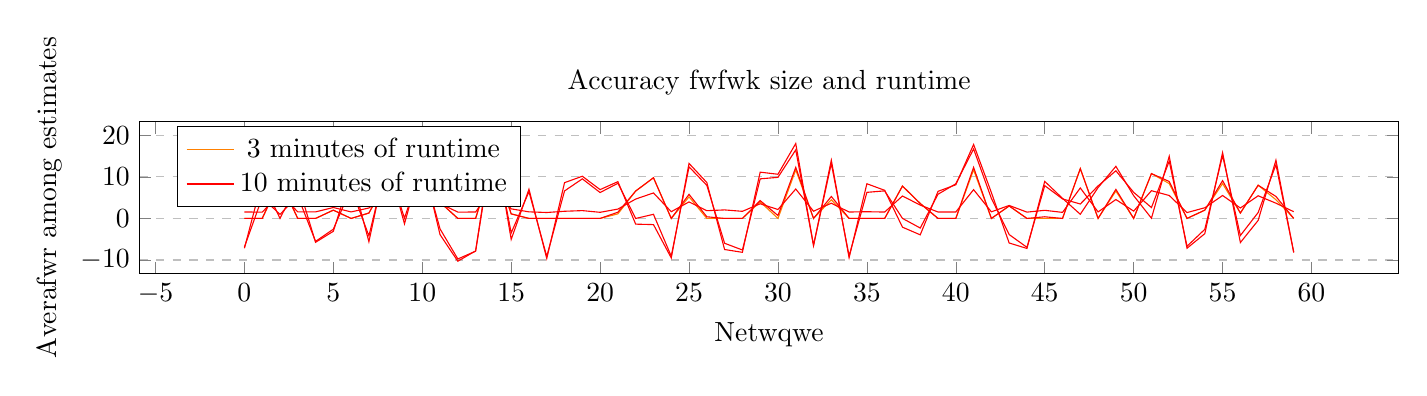
\begin{tikzpicture}
		\begin{axis}[
			title={Accuracy fwfwk size and runtime},
			xlabel={Netwqwe},
			ylabel={Averafwr among estimates},
			%xmin=0, xmax=0.25,
			%ymin=0.0001, ymax=1.0,
			%ymode=log,
			%xtick={0,0.05,0.1,0.15,0.2,0.25},
			%ytick={0,20,40,60,80,100},
			%yticklabel=$\pgfmathprintnumber{\tick}\%$,
			legend pos=north west,
			ymajorgrids=true,
			grid style=dashed,
			xticklabel style={/pgf/number format/fixed},
			width = 500,
			height = 100
		]
	%	\addplot [domain=5:15,dotted] {20+exp(exp(x/6.2))};
		\addplot[color=orange] coordinates {
(0,0.0)(1,0.0)(2,9.1)(3,0.0)(4,0.0)(5,2.0)(6,0.0)(7,1.3)(8,8.8)(9,7.2)(10,7.2)(11,3.9)(12,0.0)(13,0.0)(14,13.5)(15,1.1)(16,0.0)(17,0.0)(18,0.0)(19,0.0)(20,0.0)(21,1.1)(22,6.6)(23,9.8)(24,0.0)(25,5.2)(26,0.0)(27,0.0)(28,0.0)(29,4.0)(30,0.0)(31,11.7)(32,0.0)(33,4.5)(34,0.0)(35,0.0)(36,0.0)(37,7.8)(38,3.6)(39,0.0)(40,0.0)(41,11.7)(42,0.0)(43,3.0)(44,0.0)(45,-3.5527136788e-15)(46,0.0)(47,12.0)(48,0.0)(49,6.6)(50,0.0)(51,10.8)(52,8.4)(53,0.0)(54,2.0)(55,8.4)(56,1.3)(57,8.0)(58,4.5)(59,0.0)
			}node[pos=0.8](endofplotsquare){} ;
\addplot[color=red] coordinates {
(0,0.0)(1,0.0)(2,9.1)(3,0.0)(4,0.0)(5,2.0)(6,0.0)(7,1.3)(8,9.2)(9,7.2)(10,7.7)(11,3.9)(12,0.0)(13,0.0)(14,14.3)(15,1.1)(16,0.0)(17,0.0)(18,0.0)(19,0.0)(20,0.0)(21,1.5)(22,6.6)(23,9.8)(24,0.0)(25,5.8)(26,0.4)(27,0.0)(28,0.0)(29,4.3)(30,0.7)(31,12.3)(32,0.0)(33,5.3)(34,0.0)(35,0.0)(36,0.0)(37,7.8)(38,3.6)(39,0.0)(40,0.0)(41,12.3)(42,0.0)(43,3.0)(44,0.0)(45,0.4)(46,0.0)(47,12.0)(48,0.0)(49,7.0)(50,0.0)(51,10.8)(52,8.9)(53,0.0)(54,2.0)(55,9.1)(56,1.3)(57,8.0)(58,5.3)(59,0.0)
			}node[pos=0.8](endofplotsquare){} ;
\addplot[color=red] coordinates {
(0,1.55828042368)(1,1.51378390307)(2,5.89724242335)(3,1.59739817416)(4,1.57241703752)(5,2.63639541592)(6,1.57069425998)(7,2.51460535369)(8,5.74807237466)(9,5.11662397151)(10,4.80678912775)(11,3.57889142294)(12,1.53225542092)(13,1.5425)(14,7.77515548206)(15,2.30535057629)(16,1.58617144777)(17,1.42985992276)(18,1.72786663416)(19,1.88368851843)(20,1.47670862584)(21,2.25631008495)(22,4.67099674417)(23,6.13825734374)(24,1.6231804078)(25,3.98224349486)(26,1.86675135007)(27,2.05501579969)(28,1.71191569622)(29,3.5327863356)(30,2.14971927553)(31,7.08526583034)(32,1.73885278506)(33,3.66961403525)(34,1.54504123854)(35,1.61881930148)(36,1.53936502151)(37,5.40530360158)(38,3.21470257348)(39,1.54782934243)(40,1.55586928552)(41,6.93162774423)(42,1.59214090811)(43,3.13069125373)(44,1.52252011234)(45,1.95573629336)(46,1.45944830637)(47,7.34113270311)(48,1.56745675299)(49,4.55532447479)(50,1.76883332971)(51,6.68234280265)(52,5.52640188853)(53,1.41522175123)(54,2.57218198959)(55,5.52717325397)(56,2.51489487224)(57,5.45634022188)(58,3.67352365999)(59,1.62293691949)
			}node[pos=0.8](endofplotsquare){} ;
\addplot[color=red] coordinates {
(0,-7.18657325906)(1,9.10936734333)(2,0.0154577001048)(3,8.35657525165)(4,-5.74466052641)(5,-3.09706024461)(6,10.4972354392)(7,-5.60324832146)(8,14.4081814454)(9,-1.29326390424)(10,14.1741616708)(11,-3.91213868856)(12,-10.3012294742)(13,-7.81557972083)(14,20.2475741297)(15,-5.05061832051)(16,7.03476589515)(17,-9.64560698554)(18,8.613763694)(19,10.1659071297)(20,6.94014908481)(21,8.86171162256)(22,-1.37529357656)(23,-1.48409903067)(24,-9.50790609341)(25,13.2578338469)(26,8.64983465525)(27,-7.48625692709)(28,-8.16023099149)(29,11.1489499337)(30,10.6422803208)(31,18.0427826677)(32,-6.50988104492)(33,14.0355928651)(34,-9.45755431236)(35,8.35509633846)(36,6.77701477294)(37,-2.10216486564)(38,-3.94877305098)(39,6.52639477794)(40,8.10864532472)(41,17.8175448548)(42,6.23389404874)(43,-5.91451154279)(44,-7.22855975946)(45,8.92696941)(46,4.83527762134)(47,1.00404500911)(48,7.42801949162)(49,12.550966324)(50,5.48206864098)(51,0.0556137309222)(52,14.9822780268)(53,-7.17680121495)(54,-3.67178196341)(55,15.8712704166)(56,-5.80610585086)(57,-0.468133357491)(58,14.034338542)(59,-8.20772999475)
			}node[pos=0.8](endofplotsquare){} ;
\addplot[color=red] coordinates {
(0,-6.89493154762)(1,5.04268903319)(2,0.972028769841)(3,5.41843253968)(4,-5.52792989418)(5,-2.58917237855)(6,7.31814732143)(7,-4.20128075397)(8,13.4425248016)(9,0.0417471891534)(10,12.9921789021)(11,-2.52101636905)(12,-9.75983912037)(13,-7.88896676587)(14,18.9899358466)(15,-3.49210664683)(16,6.43908779762)(17,-9.16015612975)(18,6.62748875661)(19,9.53488839286)(20,6.23878769841)(21,8.46800462963)(22,-0.00978968253968)(23,0.996877314815)(24,-9.10146626984)(25,12.429577877)(26,7.97395585317)(27,-5.97840724206)(28,-7.59884887566)(29,9.53766815476)(30,9.89875049603)(31,16.5072901786)(32,-6.49119890873)(33,13.2445252976)(34,-9.02564763709)(35,6.28314980159)(36,6.63935796958)(37,0.013751984127)(38,-2.30903339947)(39,5.83215839947)(40,8.34694874339)(41,16.7391850198)(42,4.83128108466)(43,-3.88587334656)(44,-6.95309573413)(45,7.89512946429)(46,4.70475016534)(47,3.47914276696)(48,7.83959460678)(49,11.4769315476)(50,6.29048048942)(51,2.62045171958)(52,13.8020848214)(53,-6.70164649471)(54,-2.62177959656)(55,15.1610186839)(56,-4.11308068783)(57,1.42724255952)(58,12.9501597222)(59,-8.12579963324)
			}node[pos=0.8](endofplotsquare){} ;
\addlegendentry{3 minutes of runtime}
\addlegendentry{10 minutes of runtime}
		\end{axis}
		\end{tikzpicture}
		%\vspace{-18pt}
		\caption{Averafwwfwetworke minutes rufektop computer.}
		\label{fig:experiment_graph1}
    \end{figure}




\begin{figure}
\begin{tikzpicture}[>=latex',line join=bevel,scale=0.3]
%%
\node (p60) at (1377.0bp,306.0bp) [draw,ellipse] {p60};
  \node (p49) at (975.0bp,306.0bp) [draw,ellipse] {p49};
  \node (p22) at (848.0bp,234.0bp) [draw,ellipse] {p22};
  \node (p55) at (127.0bp,90.0bp) [draw,ellipse] {p55};
  \node (p25) at (1294.0bp,378.0bp) [draw,ellipse] {p25};
  \node (p24) at (27.0bp,306.0bp) [draw,ellipse] {p24};
  \node (p27) at (391.0bp,162.0bp) [draw,ellipse] {p27};
  \node (p26) at (848.0bp,162.0bp) [draw,ellipse] {p26};
  \node (p21) at (1195.0bp,306.0bp) [draw,ellipse] {p21};
  \node (p20) at (865.0bp,306.0bp) [draw,ellipse] {p20};
  \node (p23) at (920.0bp,234.0bp) [draw,ellipse] {p23};
  \node (p19) at (463.0bp,162.0bp) [draw,ellipse] {p19};
  \node (p47) at (664.0bp,90.0bp) [draw,ellipse] {p47};
  \node (p46) at (99.0bp,234.0bp) [draw,ellipse] {p46};
  \node (p45) at (755.0bp,162.0bp) [draw,ellipse] {p45};
  \node (p44) at (1060.0bp,378.0bp) [draw,ellipse] {p44};
  \node (p43) at (512.0bp,234.0bp) [draw,ellipse] {p43};
  \node (p42) at (1250.0bp,234.0bp) [draw,ellipse] {p42};
  \node (p41) at (645.0bp,162.0bp) [draw,ellipse] {p41};
  \node (p40) at (209.0bp,234.0bp) [draw,ellipse] {p40};
  \node (p57) at (190.0bp,162.0bp) [draw,ellipse] {p57};
  \node (p29) at (1068.0bp,234.0bp) [draw,ellipse] {p29};
  \node (p56) at (755.0bp,90.0bp) [draw,ellipse] {p56};
  \node (p51) at (1123.0bp,306.0bp) [draw,ellipse] {p51};
  \node (p54) at (463.0bp,18.0bp) [draw,ellipse] {p54};
  \node (p52) at (27.0bp,234.0bp) [draw,ellipse] {p52};
  \node (p35) at (947.0bp,90.0bp) [draw,ellipse] {p35};
  \node (p48) at (1322.0bp,234.0bp) [draw,ellipse] {p48};
  \node (p32) at (319.0bp,162.0bp) [draw,ellipse] {p32};
  \node (p10) at (497.0bp,306.0bp) [draw,ellipse] {p10};
  \node (p11) at (425.0bp,306.0bp) [draw,ellipse] {p11};
  \node (p12) at (99.0bp,306.0bp) [draw,ellipse] {p12};
  \node (p13) at (590.0bp,450.0bp) [draw,ellipse] {p13};
  \node (p14) at (587.0bp,234.0bp) [draw,ellipse] {p14};
  \node (p15) at (1132.0bp,378.0bp) [draw,ellipse] {p15};
  \node (p16) at (430.0bp,234.0bp) [draw,ellipse] {p16};
  \node (p17) at (171.0bp,306.0bp) [draw,ellipse] {p17};
  \node (p18) at (1195.0bp,450.0bp) [draw,ellipse] {p18};
  \node (p33) at (1267.0bp,306.0bp) [draw,ellipse] {p33};
  \node (p30) at (463.0bp,90.0bp) [draw,ellipse] {p30};
  \node (p31) at (664.0bp,234.0bp) [draw,ellipse] {p31};
  \node (p36) at (793.0bp,306.0bp) [draw,ellipse] {p36};
  \node (p37) at (292.0bp,90.0bp) [draw,ellipse] {p37};
  \node (p34) at (573.0bp,162.0bp) [draw,ellipse] {p34};
  \node (p53) at (1178.0bp,234.0bp) [draw,ellipse] {p53};
  \node (p2) at (226.0bp,378.0bp) [draw,ellipse] {p2};
  \node (p3) at (626.0bp,522.0bp) [draw,ellipse] {p3};
  \node (p1) at (626.0bp,594.0bp) [draw,ellipse] {p1};
  \node (p6) at (728.0bp,378.0bp) [draw,ellipse] {p6};
  \node (p7) at (683.0bp,306.0bp) [draw,ellipse] {p7};
  \node (p4) at (1060.0bp,450.0bp) [draw,ellipse] {p4};
  \node (p5) at (662.0bp,450.0bp) [draw,ellipse] {p5};
  \node (p50) at (99.0bp,162.0bp) [draw,ellipse] {p50};
  \node (p8) at (459.0bp,378.0bp) [draw,ellipse] {p8};
  \node (p9) at (988.0bp,378.0bp) [draw,ellipse] {p9};
  \node (p38) at (554.0bp,90.0bp) [draw,ellipse] {p38};
  \node (p28) at (920.0bp,162.0bp) [draw,ellipse] {p28};
  \node (p39) at (738.0bp,234.0bp) [draw,ellipse] {p39};
  \node (p58) at (27.0bp,162.0bp) [draw,ellipse] {p58};
  \node (p59) at (100.0bp,18.0bp) [draw,ellipse] {p59};
  \draw [] (p30) ..controls (463.0bp,61.0bp) and (463.0bp,47.288bp)  .. (p54);
  \draw [] (p18) ..controls (1231.3bp,423.58bp) and (1257.8bp,404.33bp)  .. (p25);
  \draw [] (p23) ..controls (920.0bp,205.0bp) and (920.0bp,191.29bp)  .. (p28);
  \draw [] (p33) ..controls (1260.2bp,277.13bp) and (1256.8bp,262.93bp)  .. (p42);
  \draw [] (p6) ..controls (710.4bp,349.84bp) and (700.91bp,334.66bp)  .. (p7);
  \draw [] (p8) ..controls (473.98bp,349.63bp) and (481.79bp,334.83bp)  .. (p10);
  \draw [] (p21) ..controls (1188.2bp,277.13bp) and (1184.8bp,262.93bp)  .. (p53);
  \draw [] (p9) ..controls (982.73bp,348.83bp) and (980.21bp,334.86bp)  .. (p49);
  \draw [] (p15) ..controls (1128.4bp,349.0bp) and (1126.7bp,335.29bp)  .. (p51);
  \draw [] (p2) ..controls (168.68bp,361.53bp) and (110.8bp,343.75bp)  .. (63.0bp,324.0bp) .. controls (58.221bp,322.03bp) and (53.197bp,319.69bp)  .. (p24);
  \draw [] (p6) ..controls (775.14bp,353.22bp) and (818.07bp,330.66bp)  .. (p20);
  \draw [] (p6) ..controls (684.72bp,361.05bp) and (658.96bp,346.35bp)  .. (647.0bp,324.0bp) .. controls (634.54bp,300.73bp) and (645.39bp,269.79bp)  .. (p31);
  \draw [] (p55) ..controls (116.14bp,61.042bp) and (110.77bp,46.714bp)  .. (p59);
  \draw [] (p5) ..controls (622.49bp,393.1bp) and (551.17bp,290.41bp)  .. (p43);
  \draw [] (p25) ..controls (1283.1bp,349.04bp) and (1277.8bp,334.71bp)  .. (p33);
  \draw [] (p9) ..controls (1013.7bp,363.92bp) and (1019.0bp,361.66bp)  .. (1024.0bp,360.0bp) .. controls (1112.7bp,330.81bp) and (1142.3bp,353.19bp)  .. (1231.0bp,324.0bp) .. controls (1236.0bp,322.34bp) and (1241.3bp,320.08bp)  .. (p33);
  \draw [] (p46) ..controls (99.0bp,205.0bp) and (99.0bp,191.29bp)  .. (p50);
  \draw [] (p17) ..controls (185.98bp,277.63bp) and (193.79bp,262.83bp)  .. (p40);
  \draw [] (p23) ..controls (942.25bp,208.15bp) and (951.69bp,194.23bp)  .. (956.0bp,180.0bp) .. controls (963.37bp,155.65bp) and (957.81bp,126.08bp)  .. (p35);
  \draw [] (p19) ..controls (463.0bp,133.0bp) and (463.0bp,119.29bp)  .. (p30);
  \draw [] (p34) ..controls (565.38bp,133.13bp) and (561.63bp,118.93bp)  .. (p38);
  \draw [] (p8) ..controls (445.42bp,349.25bp) and (438.49bp,334.56bp)  .. (p11);
  \draw [] (p40) ..controls (201.38bp,205.13bp) and (197.63bp,190.93bp)  .. (p57);
  \draw [] (p13) ..controls (589.18bp,391.3bp) and (587.82bp,292.9bp)  .. (p14);
  \draw [] (p1) ..controls (626.0bp,565.0bp) and (626.0bp,551.29bp)  .. (p3);
  \draw [] (p24) ..controls (27.0bp,277.0bp) and (27.0bp,263.29bp)  .. (p52);
  \draw [] (p4) ..controls (1087.5bp,422.51bp) and (1104.5bp,405.46bp)  .. (p15);
  \draw [] (p7) ..controls (704.48bp,277.88bp) and (716.58bp,262.04bp)  .. (p39);
  \draw [] (p5) ..controls (687.39bp,422.3bp) and (702.64bp,405.66bp)  .. (p6);
  \draw [] (p31) ..controls (674.84bp,205.93bp) and (679.09bp,192.43bp)  .. (681.0bp,180.0bp) .. controls (683.43bp,164.19bp) and (683.43bp,159.81bp)  .. (681.0bp,144.0bp) .. controls (679.09bp,131.57bp) and (674.84bp,118.07bp)  .. (p47);
  \draw [] (p16) ..controls (414.54bp,205.46bp) and (406.38bp,190.39bp)  .. (p27);
  \draw [] (p21) ..controls (1150.7bp,280.88bp) and (1112.3bp,259.11bp)  .. (p29);
  \draw [] (p31) ..controls (656.38bp,205.13bp) and (652.63bp,190.93bp)  .. (p41);
  \draw [] (p3) ..controls (640.37bp,493.25bp) and (647.72bp,478.56bp)  .. (p5);
  \draw [] (p18) ..controls (1195.0bp,404.06bp) and (1195.0bp,351.7bp)  .. (p21);
  \draw [] (p1) ..controls (645.2bp,566.82bp) and (654.53bp,552.86bp)  .. (662.0bp,540.0bp) .. controls (679.96bp,509.06bp) and (684.31bp,501.05bp)  .. (698.0bp,468.0bp) .. controls (708.15bp,443.5bp) and (717.4bp,414.22bp)  .. (p6);
  \draw [] (p39) ..controls (744.82bp,205.13bp) and (748.17bp,190.93bp)  .. (p45);
  \draw [] (p16) ..controls (390.12bp,208.13bp) and (358.61bp,187.69bp)  .. (p32);
  \draw [] (p6) ..controls (731.19bp,332.06bp) and (734.83bp,279.7bp)  .. (p39);
  \draw [] (p1) ..controls (535.49bp,545.12bp) and (316.39bp,426.81bp)  .. (p2);
  \draw [] (p52) ..controls (27.0bp,205.0bp) and (27.0bp,191.29bp)  .. (p58);
  \draw [] (p3) ..controls (588.72bp,501.17bp) and (567.4bp,486.27bp)  .. (554.0bp,468.0bp) .. controls (520.67bp,422.56bp) and (505.49bp,355.92bp)  .. (p10);
  \draw [] (p20) ..controls (858.18bp,277.13bp) and (854.83bp,262.93bp)  .. (p22);
  \draw [] (p15) ..controls (1156.2bp,350.3bp) and (1170.8bp,333.66bp)  .. (p21);
  \draw [] (p25) ..controls (1302.9bp,332.46bp) and (1313.1bp,279.9bp)  .. (p48);
  \draw [] (p9) ..controls (1025.8bp,339.88bp) and (1068.4bp,298.32bp)  .. (1087.0bp,288.0bp) .. controls (1138.3bp,259.51bp) and (1159.3bp,273.21bp)  .. (1214.0bp,252.0bp) .. controls (1219.0bp,250.08bp) and (1224.1bp,247.71bp)  .. (p42);
  \draw [] (p2) ..controls (288.36bp,355.44bp) and (363.01bp,328.43bp)  .. (p11);
  \draw [] (p16) ..controls (443.18bp,205.25bp) and (449.91bp,190.56bp)  .. (p19);
  \draw [] (p3) ..controls (730.07bp,504.74bp) and (956.1bp,467.24bp)  .. (p4);
  \draw [] (p2) ..controls (220.62bp,332.46bp) and (214.42bp,279.9bp)  .. (p40);
  \draw [] (p17) ..controls (169.16bp,269.66bp) and (168.93bp,240.67bp)  .. (173.0bp,216.0bp) .. controls (175.05bp,203.59bp) and (179.3bp,190.09bp)  .. (p57);
  \draw [] (p4) ..controls (1060.0bp,421.0bp) and (1060.0bp,407.29bp)  .. (p44);
  \draw [] (p5) ..controls (748.85bp,430.82bp) and (901.15bp,397.18bp)  .. (p9);
  \draw [] (p16) ..controls (464.42bp,211.4bp) and (484.43bp,196.36bp)  .. (499.0bp,180.0bp) .. controls (519.1bp,157.44bp) and (536.14bp,126.57bp)  .. (p38);
  \draw [] (p2) ..controls (241.98bp,308.26bp) and (276.02bp,159.72bp)  .. (p37);
  \draw [] (p33) ..controls (1288.5bp,277.88bp) and (1300.6bp,262.04bp)  .. (p48);
  \draw [] (p22) ..controls (848.0bp,205.0bp) and (848.0bp,191.29bp)  .. (p26);
  \draw [] (p3) ..controls (724.81bp,512.8bp) and (928.02bp,492.89bp)  .. (1096.0bp,468.0bp) .. controls (1120.9bp,464.31bp) and (1149.1bp,459.08bp)  .. (p18);
  \draw [] (p6) ..controls (753.01bp,350.3bp) and (768.03bp,333.66bp)  .. (p36);
  \draw [] (p32) ..controls (308.14bp,133.04bp) and (302.77bp,118.71bp)  .. (p37);
  \draw [] (p12) ..controls (99.0bp,277.0bp) and (99.0bp,263.29bp)  .. (p46);
  \draw [] (p11) ..controls (457.44bp,279.15bp) and (479.61bp,260.81bp)  .. (p43);
  \draw [] (p20) ..controls (839.14bp,292.29bp) and (833.95bp,289.92bp)  .. (829.0bp,288.0bp) .. controls (774.3bp,266.79bp) and (756.92bp,272.63bp)  .. (702.0bp,252.0bp) .. controls (696.67bp,250.0bp) and (691.06bp,247.54bp)  .. (p31);
  \draw [] (p20) ..controls (886.48bp,277.88bp) and (898.58bp,262.04bp)  .. (p23);
  \draw [] (p50) ..controls (110.15bp,133.33bp) and (115.81bp,118.77bp)  .. (p55);
  \draw [] (p28) ..controls (930.86bp,133.04bp) and (936.23bp,118.71bp)  .. (p35);
  \draw [] (p9) ..controls (1012.9bp,333.2bp) and (1043.1bp,278.76bp)  .. (p29);
  \draw [] (p2) ..controls (181.7bp,352.88bp) and (143.29bp,331.11bp)  .. (p12);
  \draw [] (p41) ..controls (652.62bp,133.13bp) and (656.37bp,118.93bp)  .. (p47);
  \draw [] (p25) ..controls (1325.3bp,350.86bp) and (1346.1bp,332.8bp)  .. (p60);
  \draw [] (p3) ..controls (611.63bp,493.25bp) and (604.28bp,478.56bp)  .. (p13);
  \draw [] (p6) ..controls (797.57bp,364.64bp) and (881.15bp,345.82bp)  .. (901.0bp,324.0bp) .. controls (918.84bp,304.39bp) and (921.53bp,272.37bp)  .. (p23);
  \draw [] (p5) ..controls (635.81bp,436.29bp) and (630.79bp,433.96bp)  .. (626.0bp,432.0bp) .. controls (576.78bp,411.87bp) and (517.07bp,394.09bp)  .. (p8);
  \draw [] (p10) ..controls (530.29bp,279.37bp) and (553.78bp,260.58bp)  .. (p14);
  \draw [] (p3) ..controls (572.04bp,509.86bp) and (527.99bp,495.37bp)  .. (500.0bp,468.0bp) .. controls (479.62bp,448.07bp) and (468.43bp,416.15bp)  .. (p8);
  \draw [] (p11) ..controls (427.01bp,277.0bp) and (427.97bp,263.29bp)  .. (p16);
  \draw [] (p45) ..controls (755.0bp,133.0bp) and (755.0bp,119.29bp)  .. (p56);
  \draw [] (p50) ..controls (93.891bp,133.6bp) and (91.891bp,120.1bp)  .. (91.0bp,108.0bp) .. controls (89.824bp,92.043bp) and (89.68bp,87.945bp)  .. (91.0bp,72.0bp) .. controls (92.003bp,59.876bp) and (94.253bp,46.376bp)  .. (p59);
  \draw [] (p2) ..controls (204.52bp,349.88bp) and (192.42bp,334.04bp)  .. (p17);
  \draw [] (p16) ..controls (478.6bp,209.53bp) and (524.11bp,186.62bp)  .. (p34);
%
\end{tikzpicture}

\caption{blasasf}
\end{figure}


\begin{figure}
\centering
\begin{tikzpicture}
\begin{axis}[width=6cm, height=6cm, view={30}{30},
%colormap/viridis,
point meta min=-1.0, point meta max=9.0,
colorbar,
grid=major]
\addplot3[only marks, scatter]
table[x index=0, y index=1, z index=2, point meta=z, col sep=comma]{data/lmp_out_csv.csv};
\end{axis}
\end{tikzpicture}

\begin{tikzpicture}
\begin{axis}[width=6cm, height=6cm, view={30}{30},
%colormap/viridis,
point meta min=-1.0, point meta max=9.0,
colorbar,
grid=major]
\addplot3[only marks, scatter]
table[x index=0, y index=1, z index=2, point meta=z, col sep=comma]{data/vcg_out_csv.csv};
\end{axis}
\end{tikzpicture}

\begin{tikzpicture}
\begin{axis}[width=6cm, height=6cm, view={30}{30},
%colormap/viridis,
point meta min=-1.0, point meta max=9.0,
colorbar,
grid=major]
\addplot3[only marks, scatter]
table[x index=0, y index=1, z index=2, point meta=z, col sep=comma]{data/gnk_out_csv.csv};
\end{axis}
\end{tikzpicture}
\caption{asdfa}
\end{figure}






%point meta min=-0.1, point meta max=1.0,
%colorbar horizontal,
%colorbar,
%colorbar style={
%	at={(1.07,0.64)},
	%title=Advantage,
	%ylabel=Z-value,
	%ytick={-1,-0.75,...,1},
%	height=0.52*\pgfkeysvalueof{/pgfplots/parent axis height},
%	xticklabel style={
%		text width=2.5em,
		%align=below,
		%anchor=north west,
%		/pgf/number format/.cd,
%		fixed,
%		fixed zerofill
%	}
%}


In this section we give some results of the utility imputations on larger and randomly generated networks between modified-GNK, VCG and LMP.
Primarily from this exersize we are able to glimse of some of the distinct features of these solutions when applied to a large number of players.

Particular things which we note are:

\begin{enumerate}
\item	The GNK value ascribes negative utilities
\item	the VCG and LMP are similar
\item	The GNK has a majority-rule effect between consumers and generators
\item	LMP and shapley value are related
\item	GNK seems to feature entirely different dynamics, and sometimes appears to be inverted with respect to rewards
\end{enumerate}

\section{Discussion and Conclusion}\label{sec:GNK_value_discussion}




And the error of using this modification as a proxy for the more original GNK value was calculated for randomly generated networks as shown in Figure \ref{fig:performance_graph5}.
From this graph it is noticed that the GNK and modified GNK values feature similarity which seems to increase with the size of the network under consideration --- although it is increasingly difficult to confirm this for networks with a size greater than 13.
This limited observation coincides with expectations that the possible strategic counter-considerations in the minimax optimizations become less relevant in the context of larger networks.
It is hence suspected that this modified GNK value may be an appropriate proxy for the GNK value in larger networks.



GNK value incentive incompatability, and it is important to note that our paper does not address the potential consequences of this.
While there does exist some work on similar solution concepts that are incentive compatible \cite{myerson1,Salamanca2019} their investigation and evaluation in the context of electricity networks remain a topic for further investigation.



\begin{enumerate}
\item	GNK value is hard to compute, sampling and proxy extend this to about 100 to 150, but not easily beyond, which still is practically limited; and still isnt escaping NP-hard nature of the problem. which VCG and LMP potentially avoid
\item	GNK value is interesting, and involuted way of total bargaining solution, raising the question of how much the group formulation is a relevent moral reference point
\item	GNK value seems to have an evident `majority-rule' issue (atleast in the proxy), it remains to be seen if it holds in the normal version, but since it dosnt scale beyond 15 it seems impossible to really know. it may be very possible to mediate this by weighting individuals in the shapley value formulation.
\item	GNK is incentive incompatable, and hence there is raised big questions about how badly it would perform in practice, and under strategising of the agents. atleast in VCG it is somewhat mitigated by incentive compatability, but not group incentive compatability, and LMP is known to limit to VCG in the limit of large markets where each player is small; but with GNK it could be unbounded dynamics under strategising.
\item	GNK seems to violate an individual rationality constraint, in that it is possible for participants to walk away with less than they started with, leaving them regretting partaking in the system. when designing GNK for electricity systems, it was hoped that invidiual rationality would `fall out', and in the neyman-kohlberg formulation it might well fall out, in that the most any agent can threaten to do is to not particiapte in the system, whereas under GNK value, the power conservation constraint allows participants to extortionately threaten to oversupply others, leaving them worse off then when they were before. this is a major ethical failing.
\end{enumerate}

In comjunction with Chapter \ref{}, we see that althought the GNK value satisfies many ethical pricniples including hard efficiency, formal equality, and consistent reference point.
ultimately it fails to encode any notion of `euvoluntary' exchange as it violates individual rationality.
Additionally, we could hardly imagine any electricity system where participants could be left worse-off for participanting without social disturbance or riots. and while it may allow a survival of the fittest, freedom to profit, it ultimately would fail to enhance the freedom of society, and fails wider social equality considerations. 

the GNK value is intricate and total considered bargaining solution, involving the calculus of what everybody could possibly do and the value that each and every participant values each and every possible combination of actions which they could bring about.
It is computationally difficult to apply to real and large electricity networks, although this is something which is potentially subject to be mitigated with momre compute power and proxies and sampling to its total calculation.
However ultimately its formulation encodes a specific type of extoritionate principle which makes it ethically untenuous.

reflectively, it is interesting how perfect competition may or may not coincide with what is equal and ethical.
and the question of when and where these two coincide, and if they might coincide in the context of electricity networks was part of the motivation of this work.

